\documentclass{article}      % Specifies the document class

%%%%%%%%%%%%%%%%% CJK 中文版面控制  %%%%%%%%%%%%%%%%%%%%%%%%%%%%%%
%\usepackage{CJK} % CTEX-CJK 中文支持                            %
\usepackage{xeCJK} % seperate the english and chinese		 %
%\usepackage{CJKutf8} % Texlive 中文支持                         %
\usepackage{CJKnumb} %中文序号                                   %
\usepackage{indentfirst} % 中文段落首行缩进                      %
%\setlength\parindent{22pt}       % 段落起始缩进量               %
\renewcommand{\baselinestretch}{1.2} % 中文行间距调整            %
\setlength{\textwidth}{16cm}                                     %
\setlength{\textheight}{24cm}                                    %
\setlength{\topmargin}{-1cm}                                     %
\setlength{\oddsidemargin}{0.1cm}                                %
\setlength{\evensidemargin}{\oddsidemargin}                      %
%%%%%%%%%%%%%%%%%%%%%%%%%%%%%%%%%%%%%%%%%%%%%%%%%%%%%%%%%%%%%%%%%%

\usepackage{amsmath,amsthm,amsfonts,amssymb,bm}          %数学公式
\usepackage{mathrsfs}                                    %英文花体
\usepackage{xcolor}                                        %使用默认允许使用颜色
%\usepackage{hyperref} 
\usepackage{graphicx}
\usepackage{subfigure}           %图片跨页
\usepackage{animate}		 %插入动画
\usepackage{caption}
\captionsetup{font=footnotesize}

%\usepackage[version=3]{mhchem}		%化学公式
\usepackage{chemfig}		%化学公式

\usepackage{fontspec} % use to set font
%\setCJKmainfont{SimSun}
\setCJKmainfont{SimHei}
\XeTeXlinebreaklocale "zh"  % Auto linebreak for chinese
\XeTeXlinebreakskip = 0pt plus 1pt % Auto linebreak for chinese

\usepackage{longtable}                                   %使用长表格
\usepackage{multirow}
\usepackage{makecell}		%允许单元格内换行

%%%%%%%%%%%%%%%%%%%%%%%%%  参考文献引用 %%%%%%%%%%%%%%%%%%%%%%%%%%%
%%尽量使用 BibTeX(含有超链接,数据库的条目URL即可)                %
%%%%%%%%%%%%%%%%%%%%%%%%%%%%%%%%%%%%%%%%%%%%%%%%%%%%%%%%%%%%%%%%%%%

\usepackage[numbers,sort&compress]{natbib} %紧密排列             %
\usepackage[sectionbib]{chapterbib}        %每章节单独参考文献   %
\usepackage{hypernat}                                                                         %
\usepackage[bookmarksopen=true,pdfstartview=FitH,CJKbookmarks]{hyperref}              %
\hypersetup{bookmarksnumbered,colorlinks,linkcolor=green,citecolor=blue,urlcolor=red}         %
%参考文献含有超链接引用时需要下列宏包,注意与natbib有冲突        %
%\usepackage[dvipdfm]{hyperref}                                  %
%\usepackage{hypernat}                                           %
\newcommand{\upcite}[1]{\hspace{0ex}\textsuperscript{\cite{#1}}} %

%%%%%%%%%%%%%%%%%%%%%%%%%%%%%%%%%%%%%%%%%%%%%%%%%%%%%%%%%%%%%%%%%%%%%%%%%%%%%%%%%%%%%%%%%%%%%%%
%\AtBeginDvi{\special{pdf:tounicode GBK-EUC-UCS2}} %CTEX用dvipdfmx的话,用该命令可以解决      %
%						   %pdf书签的中文乱码问题		      %
%%%%%%%%%%%%%%%%%%%%%%%%%%%%%%%%%%%%%%%%%%%%%%%%%%%%%%%%%%%%%%%%%%%%%%%%%%%%%%%%%%%%%%%%%%%%%%%

%%%%%%%%%%%%%%%%%%%%%  % EPS 图片支持  %%%%%%%%%%%%%%%%%%%%%%%%%%%
\usepackage{graphicx}                                            %
%%%%%%%%%%%%%%%%%%%%%%%%%%%%%%%%%%%%%%%%%%%%%%%%%%%%%%%%%%%%%%%%%%


\begin{document}
%\CJKindent     %在CJK环境中,中文段落起始缩进2个中文字符
%\indent
\graphicspath{{Figures/}}
%
\renewcommand{\abstractname}{\small{\CJKfamily{hei} 摘\quad 要}} %\CJKfamily{hei} 设置中文字体,字号用\big \small来设
\renewcommand{\refname}{\centering\CJKfamily{hei} 参考文献}
%\renewcommand{\figurename}{\CJKfamily{hei} 图.}
\renewcommand{\figurename}{{\bf Fig}.}
%\renewcommand{\tablename}{\CJKfamily{hei} 表.}
\renewcommand{\tablename}{{\bf Tab}.}

%将图表的Caption写成 图(表) Num. 格式
\makeatletter
\long\def\@makecaption#1#2{%
  \vskip\abovecaptionskip
  \sbox\@tempboxa{#1. #2}%
  \ifdim \wd\@tempboxa >\hsize
    #1. #2\par
  \else
    \global \@minipagefalse
    \hb@xt@\hsize{\hfil\box\@tempboxa\hfil}%
  \fi
  \vskip\belowcaptionskip}
\makeatother

\newcommand{\keywords}[1]{{\hspace{0\ccwd}\small{\CJKfamily{hei} 关键词:}{\hspace{2ex}{#1}}\bigskip}}

%%%%%%%%%%%%%%%%%%中文字体设置%%%%%%%%%%%%%%%%%%%%%%%%%%%
%默认字体 defalut fonts \TeX 是一种排版工具 \\		%
%{\bfseries 粗体 bold \TeX 是一种排版工具} \\		%
%{\CJKfamily{song}宋体 songti \TeX 是一种排版工具} \\	%
%{\CJKfamily{hei} 黑体 heiti \TeX 是一种排版工具} \\	%
%{\CJKfamily{kai} 楷书 kaishu \TeX 是一种排版工具} \\	%
%{\CJKfamily{fs} 仿宋 fangsong \TeX 是一种排版工具} \\	%
%%%%%%%%%%%%%%%%%%%%%%%%%%%%%%%%%%%%%%%%%%%%%%%%%%%%%%%%%

%\addcontentsline{toc}{section}{Bibliography}

%-------------------------------The Title of The Paper-----------------------------------------%
\title{基于\rm{VASP~}软件的对称性分析程序}
%----------------------------------------------------------------------------------------------%

%----------------------The Authors and the address of The Paper--------------------------------%
\author{
\small
%Author1, Author2, Author3\footnote{Communication author's E-mail} \\    %Authors' Names	       %
\small
%(The Address,City Post code)						%Address	       %
}
\date{}					%if necessary					       %
%----------------------------------------------------------------------------------------------%
\maketitle

%-------------------------------------------------------------------------------The Abstract and the keywords of The Paper----------------------------------------------------------------------------%
%\begin{abstract}
%The content of the abstract
%\end{abstract}

%\keywords {Keyword1; Keyword2; Keyword3}
%-----------------------------------------------------------------------------------------------------------------------------------------------------------------------------------------------------%
\tableofcontents %—— 制作目录(目录是根据标题自动生成的)
\newpage
%----------------------------------------------------------------------------------------The Body Of The Paper----------------------------------------------------------------------------------------%
\section{Introduction}
\fbox{主程序\textbf{Kpoint\_PATH}}是在\textrm{VASP~}软件的(点群)对称性分析模块基础上发展的,它可以根据输入结构文件(\textrm{POSCAR~}格式),确定晶体所属晶系、\textrm{Bravais~}格子类型和点群、空间群,并产生标准化能带所需要的\textrm{K-path}\upcite{CMS49-299_2010}。

\fbox{主程序\textbf{Kpoint\_PATH~}}的结构见图\ref{Fig:Fig_Flow}。其主要结构分为如下部分
\begin{itemize}
	\item \textrm{POSCAR~}文件的读入
	\item 晶体所属点群对称性的判断
	\item 晶体所属空间群对称性的指认
	\item 标准化\textrm{K-path}的生成
\end{itemize}

运行\textcolor{blue}{\textbf{Kpoint\_PATH~}}所需要的输入文件:~\;\;\textcolor{purple}{\textrm{POSCAR~}}(\textbf{15}号文件)\\
输出文件主要是两个:~
\begin{enumerate}
	\item 对称性分析和点群和空间群信息:~\textcolor{purple}{\textrm{OUTKPATH~}}(\textbf{8}号文件)
	\item 标准化能带所需的$\vec k$-点路径:~\textcolor{purple}{\textrm{KPOINTS\_BAND~}}(\textbf{12}号文件)
\end{enumerate}

\begin{figure}[h!]
\centering
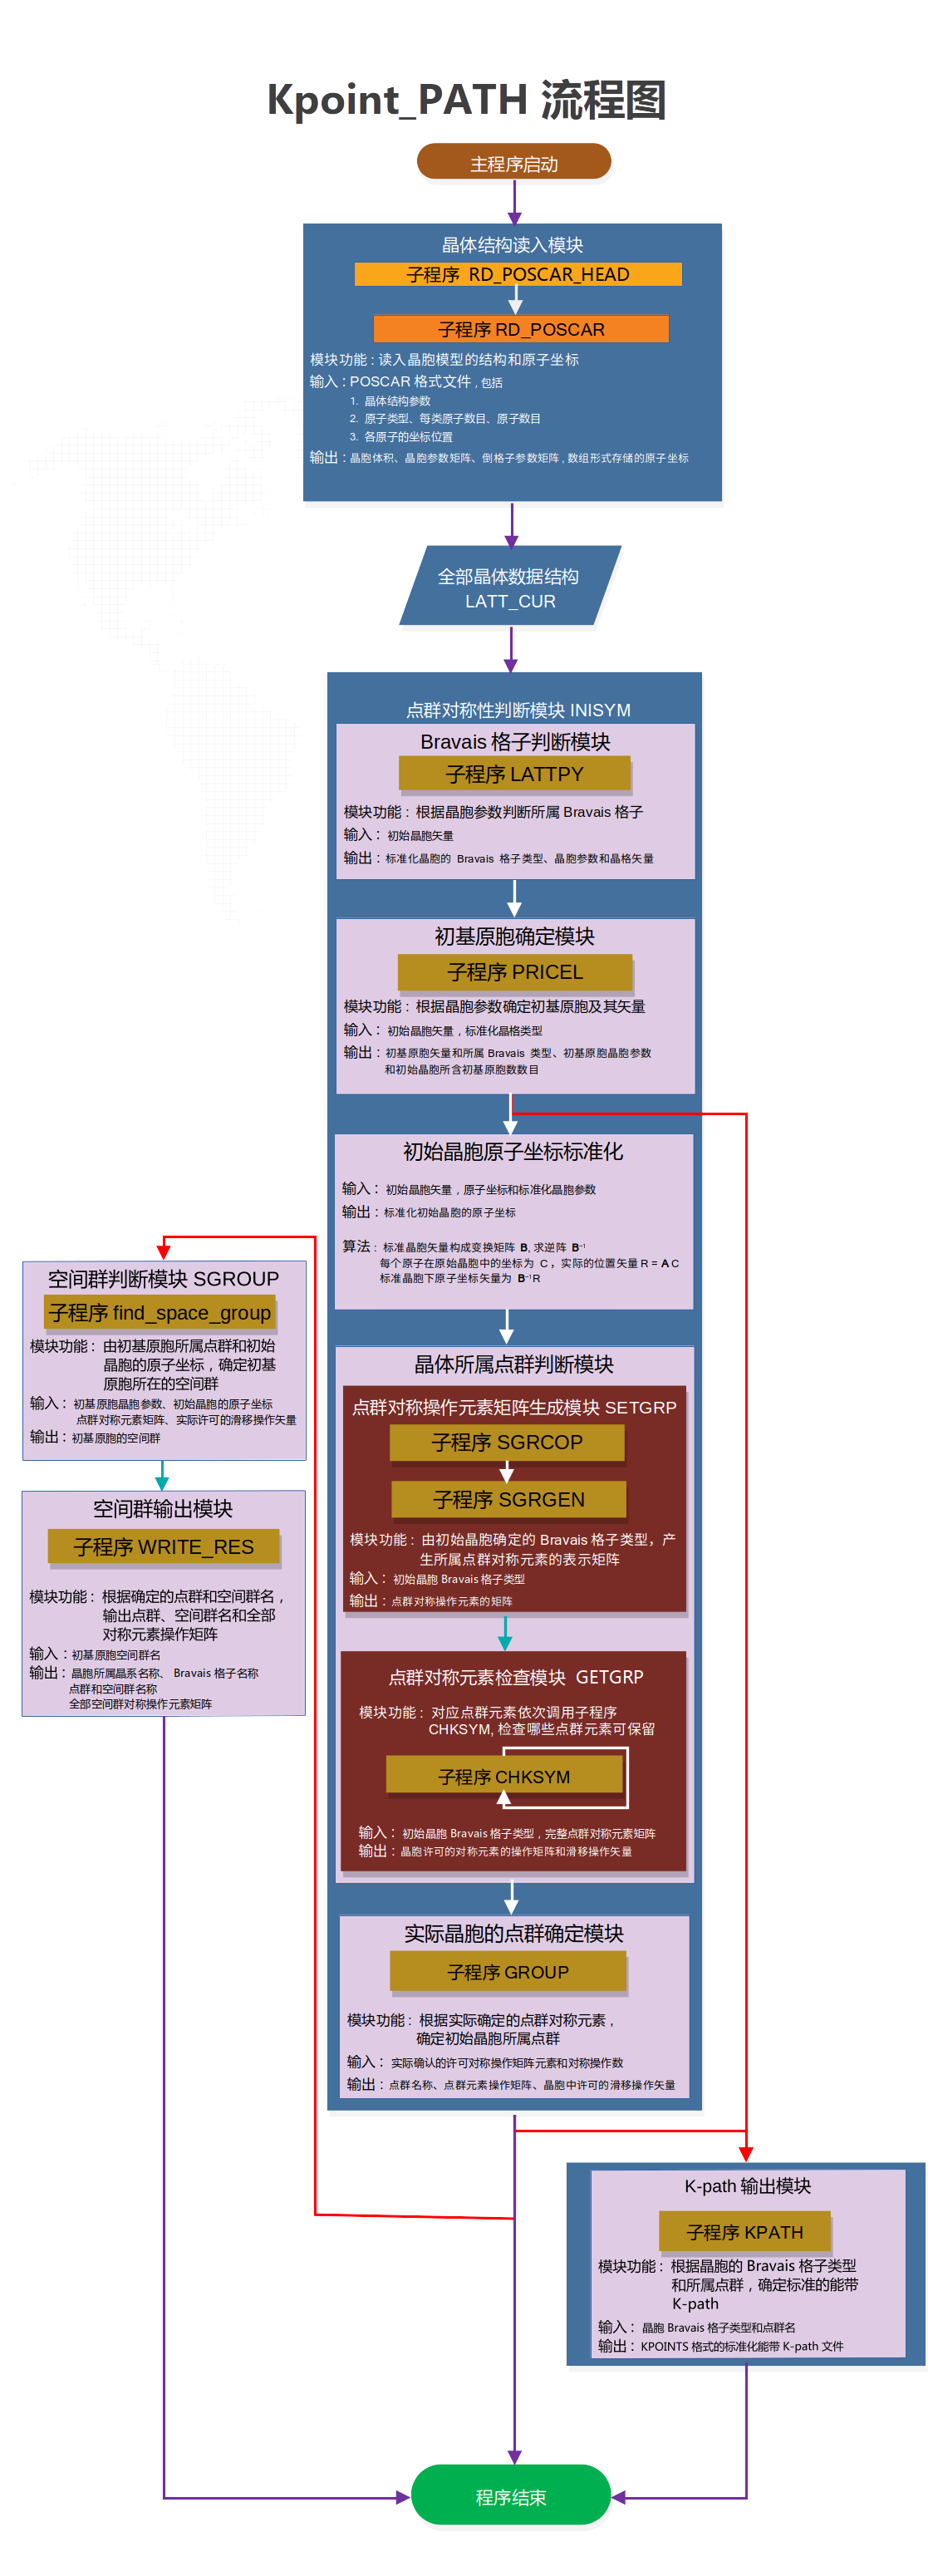
\includegraphics[height=8.80in,width=3.75in,viewport=0 0 840 2255,clip]{VASP_sym-detail.png}
\caption{\small The Flow of the symmetry analysis.}%(与文献\cite{EPJB33-47_2003}图1对比)
\label{Fig:Fig_Flow}
\end{figure}

\fbox{主程序\textbf{Kpoint\_PATH}}中的变量:\\
\begin{itemize}
	\item \textbf{IU6/IU8}~是\textbf{整型变量}:~表示文件号
	\item \textbf{FILE}~是文件号对应的文件名\;\;\;\; \textbf{STATUS}~文件状态
	\item \textbf{LATT\_CUR}~是关于晶体参数的\textbf{数据结构}
	\item \textbf{SYMM}~是关于晶体点群对称性的\textbf{数据结构}
	\item \textbf{IPTYP}~是\textbf{整型变量}:~表示元素类型变量,取值 $1\sim\mathrm{NTYPD}$
	\item \textbf{NIOND}~是\textbf{整型变量}:~记录\textrm{POSCAR}~中总的原子数
	\item \textbf{NIONPD}~是\textbf{整型变量}:~记录\textrm{POSCAR}~中每一类原子的数目
	\item \textbf{NTYPPD}~是\textbf{整型变量}:~记录\textrm{POSCAR}~中总的原子数
	\item \textbf{CELLDM(6)}是\textbf{固定数组}:~记录晶胞参数$a,b,c;~\alpha,\beta,\gamma$
	\item \textbf{CELLDMK(6)}是\textbf{固定数组}:~记录倒格子的晶胞参数$a^{\vec k},b^{\vec k},c^{\vec k};~\alpha^{\vec k},\beta^{\vec k},\gamma^{\vec k}$
	\item \textbf{PCELLDM(6)}是\textbf{固定数组}:~记录初基原胞的晶胞的参数$a_p,b_p,c_p;~\alpha_p,\beta_p,\gamma_p$
	\item \textbf{PCELLDMK(6)}是\textbf{固定数组}:~记录倒格子初基原胞的晶胞的参数$a_p^{\vec k},b_p^{\vec k},c_p^{\vec k};~\alpha_p^{\vec k},\beta_p^{\vec k},\gamma_p^{\vec k}$
\end{itemize}

\fbox{主程序\textbf{Kpoint\_PATH}}的内容(打开\textbf{8}号文件(\textrm{OUTKPATH~})后):~

\section{读入\bf{POSCAR~}文件模块}
该模块主要包括两部分
\begin{enumerate}
	\item 读入晶格矢量(晶胞参数)和元素类型、原子数目的信息:~\fbox{子程序\textbf{RD\_POSCAR\_HEAD}}
	\item 读入原子坐标:~\fbox{子程序\textbf{RD\_POSCAR}}
\end{enumerate}

\subsection{子程序\bf{RD\_POSCAR\_HEAD}分析}\label{tag:RD_POSCAR_HEAD}
\fbox{子程序\textbf{RD\_POSCAR\_HEAD}}\\
\begin{description}
	\item[输出参数:~]\textcolor{blue}{数据结构\textbf{LATT\_CUR}}:~晶格矢量信息;
	\item[输出参数:~]\textcolor{blue}{数据结构\textbf{T\_INFO}}:~晶体元素信息;
	\item[输出参数:~]\textcolor{blue}{\textrm{NIOND}}:~晶体中的原子总数;
	\item[输出参数:~]\textcolor{blue}{\textrm{NIONPD}}:~晶体中的原子总数;
	\item[输出参数:~]\textcolor{blue}{\textrm{NTYPD}}:~晶体中的元素类型;
	\item[输出参数:~]\textcolor{blue}{\textrm{NTYPPD}}:~晶体中的元素类型
\end{description}
打开\textbf{15}号文件(\textrm{POSCAR})\\
读入\textrm{POSCAR}文件第1行,记入字符串变量\textbf{CHARAC}\\
读入\textrm{POSCAR}文件第2行,记入字符串变量\textbf{INPLIN}\\
对字符串变量\textbf{INPLIN}的分析:~
通过调用\fbox{外部函数\textrm{NITEMS}},确定字符串变量\textbf{INPLIN}的个数(存入整型变量\textbf{NSCALE}),并把字符串变量\textbf{INPLIN}转成浮点型数值变量
\begin{itemize}
	\item \textbf{NSCALE}=1,\textbf{数据结构LATT\_CUR}~的成员\textbf{LATT\_CUR}\%\textrm{SCALE}赋值为浮点型变量\textbf{INPLIN}的值\footnote{这里采用的\textrm{read}格式下的~\textcolor{red}{\textrm{internal~file}}~实现对变量赋值}\\
		变量\textrm{SCALEX/Y/Z}=1
	\item \textbf{NSCALE}=3,\textbf{数据结构LATT\_CUR}~的成员\textbf{LATT\_CUR}\%\textrm{SCALE}赋值为1\\
		变量\textrm{SCALEX/Y/Z}=浮点型变量\textbf{INPLIN}的三个值
\end{itemize}
\textbf{DO}~I=1,~3循环,读入\textrm{POSCAR}文件第3$\sim$5行
\begin{description}
	\item[]记入\textbf{数据结构LATT\_CUR}~的成员\textbf{LATT\_CUR}\%\textrm{A(1:3,I)}
\end{description}
针对\textcolor{magenta}{\textbf{LATT\_CUR}\%\textrm{SCALE}<0}
\begin{description}
	\item[] \textbf{LATT\_CUR}\%\textrm{SCALE}表示晶格体积
	\item[] 调用\fbox{子程序\textbf{LATTIC}}计算由\textbf{LATT\_CUR}\%\textrm{A}确定的体积\textbf{LATT\_CUR}\%\textrm{OMEGA}
	\item[] 计算\textbf{LATT\_CUR}\%\textrm{SCALE}=$\bigg[\dfrac{|\mathbf{LATT\_CUR}\%\mathrm{SCALE}|}{|\mathbf{LATT\_CUR}\%\mathrm{OMEGA}|}\bigg]^{1/3}$
\end{description}
\textbf{DO}~\textrm{I}=1,~3循环,计算实际的\textbf{数据结构LATT\_CUR}~的成员\textbf{LATT\_CUR}\%\textrm{A(1:3,I)}(考虑\textrm{SCALE})
\begin{description}
	\item[]\textbf{LATT\_CUR}\%\textrm{A(1:3,I)}=\textbf{LATT\_CUR}\%\textrm{A(1:3,I)}*\textrm{SCALE(X/Y/Z)}*\textbf{LATT\_CUR}\%\textrm{SCALE}
\end{description}
调用\fbox{子程序\textbf{LATTIC}}计算当前\textbf{LATT\_CUR}\%\textrm{A}确定的体积\textbf{LATT\_CUR}\%\textrm{OMEGA}\\
读入\textrm{POSCAR}文件第6行,记入字符串变量\textbf{INPLIN}\\
对字符串变量\textbf{INPLIN}的分析:~
\begin{itemize}
	\item 将字符串变量\textbf{INPLIN}赋予变量\textrm{CHARAC}
	\item 检查确认字符串变量\textrm{CHARAC~}不是0-9的数字后,执行
		\begin{enumerate}
			\item 统计字符串变量的数目,记入\textbf{数据结构T\_INFO}~的成员\textbf{T\_INFO}\%\textrm{NTYP}
			\item 将字符串变量依次记入数组变量\textbf{TYPE},数组维度即\textbf{T\_INFO}\%\textrm{NTYP}
		\end{enumerate}
	\item 读入\textrm{POSCAR}文件第7行,记入字符串变量\textbf{INPLIN}
	\item 统计字符串变量的数目,要求该数据与\textbf{T\_INFO}\%\textrm{NTYP}一致
\end{itemize}
数据结构\textbf{T\_INFO}~的成员\textbf{T\_INFO}\%\textrm{NTYPP}=\textbf{T\_INFO}\%\textrm{NTYP}\\
将字符串中的数字依次记入数组变量\textbf{NITYP},数组维度也即\textbf{T\_INFO}\%\textrm{NTYP},这样就统计了\textrm{POSCAR~}文件中每一类元素的原子数目。\\
\textbf{DO}~\textrm{NI}=1,~\textbf{T\_INFO}\%\textrm{NTYP}循环,
\begin{description}
	\item[] 统计\textrm{POSCAR~}文件中全部元素的原子数目,记入变量\textbf{T\_INFO}\%\textrm{NIONS}
\end{description}
数据结构\textbf{T\_INFO}~的成员\textbf{T\_INFO}\%\textrm{NIONP}=\textbf{T\_INFO}\%\textrm{NIONS}\\
读入\textrm{POSCAR}文件第8行,记入字符串变量\textbf{CHARAC},如果字符串头字母为'S'或's'(表示'\textrm{Selective~Dynamics}'),则继续读入文件\textrm{POSCAR}第9行\\
确定整型变量参数值

\textcolor{red}{注:~}早先的\textrm{VASP~}代码在此还有包含“空球元素”的处理,这种建模实际应用中很少使用,故从略。
\begin{itemize}
	\item \textbf{NIOND}=\textbf{T\_INFO}\%NIONS\;\;离子总数
	\item \textbf{NTYPD}=\textbf{T\_INFO}\%NTYP\;\;元素类型
	\item \textbf{NIONPD}=\textbf{T\_INFO}\%NIONP\;\;离子总数
	\item \textbf{NTYPPD}=\textbf{T\_INFO}\%NTYPP\;\;元素类型
\end{itemize} 
关闭\textbf{15}号文件(\textrm{POSCAR})

\vskip 30pt
\fbox{子程序\textbf{LATTIC}}
\begin{description}
	\item[输入/输出参数:~]\textcolor{brown}{\textbf{数据结构LATT\_CUR}}:~晶格矢量信息
\end{description}
\textcolor{magenta}{晶格矢量构成的矩阵\textbf{数据结构LATT\_CUR}\%\textrm{A},表示的是\textrm{Cartesian}~坐标与\textrm{Diract}~坐标变换关系}($\mathrm{Diract}\Longrightarrow\mathrm{Cartesian}$)\\
计算晶格矢量的叉乘 
\begin{displaymath}
	\begin{aligned}
		\vec B_1^0(1:3)&=\vec A_2(1:3)\times\vec A_3(1:3)\\
		\vec B_2^0(1:3)&=\vec A_1(1:3)\times\vec A_3(1:3)\\
		\vec B_3^0(1:3)&=\vec A_1(1:3)\times\vec A_2(1:3)
	\end{aligned}
\end{displaymath}
晶格体积$\Omega=\sum\limits_{j=1}^3\vec B_1^0(j)\cdot\vec A_1(j)$\;\;即经典的体积计算公式$\Omega=\vec A_1\cdot(\vec A_2\times\vec A_3)$\\

\textcolor{red}{倒晶格矢量}的计算表达式(以单位$\dfrac{2\pi}a$为单位):~
\begin{displaymath}
	\begin{aligned}
		\vec B_1(1:3)&=\vec B_1^0(1:3)/\Omega\\%=\dfrac1{A_1(1:3)}\\
		\vec B_2(1:3)&=\vec B_2^0(1:3)/\Omega\\%=\dfrac1{A_2(1:3)}\\
		\vec B_3(1:3)&=\vec B_3^0(1:3)/\Omega\\%=\dfrac1{A_3(1:3)}
	\end{aligned}
\end{displaymath}
\textbf{倒晶格矢量构成矩阵\textbf{数据结构LATT\_CUR}}\%\textrm{B},该矩阵是表示的是正空间\textrm{Cartesian}~坐标与倒空间\textrm{Cartesian}~晶格矩阵间的逆变换关系%,($\mathrm{Cartesian}\Longrightarrow\mathrm{Diract}$)

\noindent\textbf{DO}~\textrm{I}=1,~3循环,\textrm{Cartesian~}晶格矢量和逆矢量的模量为
\begin{description}
	\item[]\textbf{LATT\_CUR}\%\textrm{ANORM}(I)=$\sqrt{\sum\limits_{j=1}^3\vec A_I(j)*\vec A_I(j)}$
	\item[]\textbf{LATT\_CUR}\%\textrm{BNORM}(I)=$\sqrt{\sum\limits_{j=1}^3\vec B_I(j)*\vec B_I(j)}$
\end{description}
\textbf{LATT\_CUR}\%\textrm{Omega}=$\Omega$

\subsection{子程序\bf{RD\_POSCAR}分析}
\fbox{子程序\textbf{RD\_POSCAR}}
\begin{description}
	\item[输出参数:~]\textcolor{blue}{数据结构\textbf{LATT\_CUR}}:~晶格矢量信息;
	\item[输出参数:~]\textcolor{blue}{数据结构\textbf{T\_INFO}}:~晶体元素信息;
	\item[输出参数:~]\textcolor{blue}{数据结构\textbf{DYN}}:~考虑动力学影响的晶格矢量信息;
	\item[输出参数:~]\textcolor{blue}{\textrm{NIOND}}:~晶体中的原子总数;
	\item[输出参数:~]\textcolor{blue}{\textrm{NIONPD}}:~晶体中的原子总数;
	\item[输出参数:~]\textcolor{blue}{\textrm{NTYPD}}:~晶体中的元素类型;
	\item[输出参数:~]\textcolor{blue}{\textrm{NTYPPD}}:~晶体中的元素类型
\end{description}
打开\textbf{15}号文件(\textrm{POSCAR})\\
读入\textrm{POSCAR}文件第1行,记入\textbf{数据结构T\_INFO}~的成员\textbf{T\_INFO}\%\textrm{SZNAM2}\\
\textcolor{red}{\fbox{子程序RD\_POSCAR}读\textrm{POSCAR}的前6行与\fbox{子程序RD\_POSCAR\_HEAD}中的方式一样,参见\ref{tag:RD_POSCAR_HEAD}}\\
\textbf{DO}~\textrm{NT}=1,~\textbf{T\_INFO}\%\textrm{NTYP}循环\\
\indent\textbf{DO}~\textrm{NI}=1,~\textbf{T\_INFO}\%\textrm{NITYP}(NT)+\textrm{NI}-1循环
	\indent \textbf{T\_INFO}\%\textrm{ITYP(NI)}=\textrm{NT}\\
	\indent 在\textbf{数据结构T\_INFO}~的成员\textbf{T\_INFO}\%\textrm{ITYP(NI)}中记入原子\textrm{ITYP(NI)}在总原子数中的序号(\textrm{NT}的值将与\textrm{POSCAR}文件中的原子坐标需要对应)\\
读入\textrm{POSCAR}文件第7行,记入字符串变量\textbf{CSEL}\\
如果字符串\textbf{CSEL}为\textrm{'S'}或\textrm{'s'}(即\textrm{'Selective~Dynamic'})则读入下一行,记入字符串变量\textbf{CSEL}\\
如果字符串\textbf{CSEL}为\textrm{'K'}或\textrm{'k'}/\textrm{'C'}或\textrm{'c'},则\textrm{CSEL='K'},表明原子采用\textrm{Cartesian~}坐标(\textbf{数据结构T\_INFO}~的成员\textbf{T\_INFO}\%\textrm{LDIRACO}=\textrm{.FALSE.})\\
如果字符串\textbf{CSEL}为其他字符,表明原子采用\textrm{Diract~}坐标(\textbf{数据结构T\_INFO}~的成员\textbf{T\_INFO}\%\textrm{LDIRACO}=\textrm{.TRUE.})\\
\textbf{DO}~\textrm{NI}=1,~\textbf{T\_INFO}\%\textrm{NIONS}循环\\
读入\textrm{POSCAR}文件余下各行,记入\textbf{数据结构T\_INFO}~的成员\textbf{T\_INFO}\%\textrm{POSITON(1:3,NI)}\\

当原子采用\textrm{Cartesian~}坐标时,完成\textrm{Cartesian~}坐标向\textrm{Diract~}变换,按两步完成:~
\begin{enumerate}
	\item \textbf{T\_INFO}\%\textrm{POSITON(1:3,NI)}=\textbf{LATT\_CUR}\%\textrm{SCALE}*\textbf{T\_INFO}\%\textrm{POSITON(1:3,NI)}*\textrm{SCALEX/Y/Z}
	\item 调用\fbox{子程序\textbf{KARDIR}}~将\textrm{Cartesian~}坐标变换为\textrm{Diract~}坐标
\end{enumerate}
调用\fbox{子程序\textbf{TOPRIM}},将原子坐标用标准的\textrm{Diract~}坐标用$(0.0,1.0)$范围内的值表示。

\textcolor{red}{注:~}\textrm{VASP~}代码在此还有包含“空球元素”和原子运动(适合分子动力学)的处理,在对称性分析代码部分从略。

\vskip 30pt
\fbox{子程序\textbf{KARDIR}}
\begin{description}
	\item[输入参数:~]\textcolor{violet}{\textrm{NIONS}}:~晶胞中的原子数目;
	\item[输入参数:~]\textcolor{violet}{变换矩阵\textrm{BASIS}}:~$\mathrm{Cartesian}\Longrightarrow\mathrm{Diract}$;
	\item[输入/输出参数:~]\textcolor{brown}{\textrm{V}}:~晶胞中的原子坐标
\end{description}
这里变换矩阵\textrm{BASIS}取的是\textbf{晶格逆变换矩阵}\textbf{LATT\_CUR}\%\textrm{B}\\
\textbf{DO}~\textrm{I}=1,~\textrm{NIONS}~循环,可将\textrm{Cartesian~}坐标变换为\textrm{Diract~}坐标
\begin{description}
	\item[] $\mathrm{V_{1:3}}=\sum\limits_{K=1}^3\textrm{V(K,I)}*\textrm{BASIS(K,1:3)}$
	\item[] $\mathrm{V(1:3,I)}=\mathrm{V_{1:3}}$
\end{description}

\vskip 30pt
\fbox{子程序\textbf{TOPRIM}}
\begin{description}
	\item[输入参数:~]\textcolor{violet}{\textrm{NIONS}}:~晶胞中的原子数目;
	\item[输入/输出参数:~]\textcolor{brown}{\textrm{POSION}}:~晶胞中的原子坐标
\end{description}
\textbf{DO}~\textrm{I}=1,~\textrm{NIONS}~循环
\begin{description}
	\item[] $\mathrm{POSION(1:3,I)}=\mod{(\mathrm{POSION(1:3,I)}+60,1.0)}$
\end{description}
该求余运算确保坐标值在$(0.0,1.0)$之间。

\section{晶体点群对称性判断模块}\label{tag:Point_symmetry}
晶体点群对称性判断由\fbox{\textbf{子程序INISYM}}~实现
\textbf{DO}~\textrm{I}=1,~3循环,将晶格矢量由\textbf{LATT\_CUR}\%\textrm{A},记入$\vec A_1(1:3)$,$\vec A_2(1:3)$,$\vec A_3(1:3)$\\

\fbox{\textbf{子程序INISYM}}主要包括如下步骤:~
\begin{enumerate}
	\item 晶胞参数的标准化,晶格所属晶系和\textrm{Bravais~}格子的确定:~\fbox{子程序\textbf{LATTYP}}
	\item 初基原胞(\textrm{primitive~cell})的确定:~\fbox{子程序\textbf{PRICEL}}
	\item 点群对称操作元素的矩阵表示:~\fbox{子程序\textbf{SETGRP}}
	\item 对群元素的逐一检查并确认:~\fbox{子程序\textbf{GETGRP}}
	\item 晶体所属点群的确认:~\fbox{子程序\textbf{GGROUP}}
\end{enumerate}

\subsection{标准化晶胞参数:}
\fbox{子程序\textbf{LATTYP}}
\begin{description}
	\item[输入/输出参数:~]\textcolor{brown}{$\vec A_1(1:3)$,$\vec A_2(1:3)$,$\vec A_3(1:3)$}:~晶格矢量
	\item[输出参数:~]\textcolor{blue}{\textrm{IBRAV~}}(ITYP):~\textrm{Bravais~}格子序号
	\item[输出参数:~]\textcolor{blue}{\textrm{CELLDM}(1:6)}:~晶胞参数数组($a,b,c;\alpha,\beta,\gamma$)
\end{description}
调用\fbox{子程序\textbf{CELVOL}},计算晶胞体积体积$\Omega$
\begin{itemize}
	\item 如果体积$|\Omega|<=1.0^{-8}$~则报错(晶胞体积为0),并将晶胞参数\textrm{CELLDM}(1:6)清零:~\textrm{CELLDM(1:6)}=0.0,程序退出执行
	\item 如果体积$\Omega< 0.0$~则表明晶胞矢量不满足坐标系的“右手定则”,翻转矢量以满足要求,即:\\$\vec A_1(1:3)=-\vec A_1(1:3)$,$\vec A_2(1:3)=-\vec A_2(1:3)$,$\vec A_3(1:3)=-\vec A_3(1:3)$
\end{itemize}
用矢量$\vec{SA}_1$,$\vec{SA}_2$,$\vec{SA}_3$记录当前矢量$\vec A_1(1:3)$,$\vec A_2(1:3)$,$\vec A_3(1:3)$\\
用矩阵$\mathbf{RB}$和矩阵$\mathbf{XB}$再次记录当前矢量$\vec A_1(1:3)$,$\vec A_2(1:3)$,$\vec A_3(1:3)$所构成的矩阵\\

\subsubsection{根据晶格矢量判断晶体所属\rm{Bravais~}格子}\label{tag:Bravais-latt}
\noindent\textcolor{purple}{初次检查晶胞矢量是否属于奇异(如晶胞矢量夹角$\alpha,\beta,\gamma$接近0$^{\circ}$或180$^{\circ}$或$c/a,b/a$特别大或特别小)}
\begin{description}
	\item[]计算矢量$\vec A_1$/$\vec A_2$/$\vec A_3$的矢量模量$|\vec A_1|$;~$|\vec A_2|$;~$|\vec A_3|$,确定晶胞参数:\\
		$a=|\vec A_1|$;~$b=|\vec A_2|$;~$c=|\vec A_3|$
	\item[]计算矢量点积:~$\vec A_1\cdot\vec A_2$;~$\vec A_3\cdot\vec A_1$;~$\vec A_3\cdot\vec A_2$
	\item[]计算矢量模量:~$|\vec A_1-\vec A_2|$;~$|\vec A_1-\vec A_3|$;~$|\vec A_2-\vec A_3|$
	\item[]计算矢量模量:~$|\vec A_1+\vec A_2-\vec A_3|$;~$|\vec A_2+\vec A_3-\vec A_1|$;~$|\vec A_1+\vec A_3-\vec A_1|$
	\item[]计算矢量点积和:~$\vec A_1\cdot\vec A_2+\vec A_3\cdot\vec A_1+\vec A_3\cdot\vec A_2$
	\item[]计算矢量夹角余弦,确定晶胞参数角度部分:\\
		$\cos\alpha=\dfrac{\vec A_1\cdot\vec A_2}{|\vec A_1|\times|\vec A_2|}$;~$\cos\beta=\dfrac{\vec A_1\cdot\vec A_3}{|\vec A_1|\times|\vec A_3|}$;~$\cos\gamma=\dfrac{\vec A_2\cdot\vec A_3}{|\vec A_2|\times|\vec A_3|}$
	\item[]计算矢量夹角余弦绝对值:\\
		$|\cos\alpha|=\left|\dfrac{\vec A_1\cdot\vec A_2}{|\vec A_1|\times|\vec A_2|}\right|$;~$|\cos\beta|=\left|\dfrac{\vec A_1\cdot\vec A_3}{|\vec A_1|\times|\vec A_3|}\right|$;~$|\cos\gamma|=\left|\dfrac{\vec A_2\cdot\vec A_3}{|\vec A_2|\times|\vec A_3|}\right|$
	\item[]检查由晶胞矢量构成的晶胞是否属于“奇异晶胞”的条件(\textcolor{purple}{用参数\textrm{ISTRGE}>0标记})
\begin{itemize}
	\item[]如果$|\cos\alpha/|$;~$|\cos\beta|$;~$|\cos\gamma|>0.995$
	\item[]如果$\dfrac ab$;~$\dfrac ac$;~$\dfrac bc$;~$\dfrac ba$;~$\dfrac ca$;~$\dfrac cb<0.001$
\end{itemize}
\end{description}

\noindent\textcolor{purple}{根据晶格矢量和晶胞参数确定晶胞所属的\textrm{Bravais~}格子类型}
\begin{description}
	\item[]如果矢量夹角余弦\underline{满足}$\cos\alpha=\cos\beta=\cos\gamma$
		\begin{description}
			\item[] 如果晶格矢量\underline{满足}$|\vec A_1|=|\vec A_2|=|\vec A_3|$
				\begin{itemize}
					\item 如果$|\cos\alpha|=0$,则属于简单立方晶胞(\textrm{Simple~Cubic~cell}),见\textrm{Fig.~}\ref{Bravais:Cubic}\\
						记录晶胞参数\textrm{CELLDM}的方式:~\textcolor{blue}{$a=b=c=|\vec A_1|;~\cos\alpha=\cos\beta=\cos\gamma=0.0$}
					\item 如果$|\cos\alpha+\dfrac13|=0$,则属于体心立方晶胞(\textrm{Body~Centered~Cubic~cell}),见\textrm{Fig.~}\ref{Bravais:body-centered Cubic}\\ 
						记录晶胞参数\textrm{CELLDM}的方式:~\textcolor{blue}{$a=b=c=\dfrac{2|\vec A_1|}{\sqrt3};~\cos\alpha=\cos\beta=\cos\gamma=0.0$}
					\item 如果$|\cos\alpha-\dfrac12|=0$,则属于面心立方晶胞(\textrm{Face~Centered~Cubic~cell}),见\textrm{Fig.~}\ref{Bravais:face-centered Cubic}\\ 
						记录晶胞参数\textrm{CELLDM}的方式:~\textcolor{blue}{$a=b=c=\sqrt2|\vec A_1|;~\cos\alpha=\cos\beta=\cos\gamma=0.0$}
					\item \underline{除此之外},则属于三方晶胞(\textrm{Rhombohedral~(Trigonal)~cell}),见\textrm{Fig.~}\ref{Bravais:rhombohedral cell}\\
						记录晶胞参数\textrm{CELLDM}:~\textcolor{blue}{$a=b=c=|\vec A_1|;~\cos\alpha=\cos\beta=\cos\gamma\neq 0.0$}
				\end{itemize}
			\item[] 如果晶格矢量\underline{\textcolor{red}{不}满足}$|\vec A_1|=|\vec A_2|=|\vec A_3|$,但晶胞参数仍要求\underline{满足}$|\cos\alpha|=0.0$
				\begin{itemize}
					\item 如果\underline{仅满足}$|\vec A_1|=|\vec A_2|$,则属于简单四方晶胞(\textrm{Simple~Tetragonal~cell}),见\textrm{Fig.~}\ref{Bravais:tetragonal cell}\\
						(\textcolor{red}{\textrm{VASP}中规定取$c$轴为特殊轴,因此取$a=b\neq c$}\\
						记录晶胞参数\textrm{CELLDM}:~\textcolor{blue}{$a=b=|\vec A_1|;~c=|\vec A_3|;~\cos\alpha=\cos\beta=\cos\gamma=0.0$})
					\item 如果$|\vec A_3|\neq|\vec A_2|\neq|\vec A_1|$,则属于简单正交晶胞(\textrm{Simple~Orthorhombic~cell}),见\textrm{Fig.~}\ref{Bravais:orthorhombic cell}\\
						(\textcolor{red}{\textrm{VASP}中规定取$a<b<c$}\\
						如果$|\vec A_3|>|\vec A_2|>|\vec A_1|$,记录晶胞参数\textrm{CELLDM}:\\
						\textcolor{blue}{$a=|\vec A_1|<b=|\vec A_2|<c=|\vec A_3|;~\cos\alpha=\cos\beta=\cos\gamma=0.0$})
				\end{itemize}
		\end{description}
	\item[] 如果矢量夹角余弦\underline{仅满足}$\cos\beta=\cos\gamma(\neq\cos\alpha)$
		\begin{description}
			\item[] 当矢量夹角余弦\underline{仍满足}$|\cos\beta|=0.0$
			\begin{description}
				\item[] 如果晶格矢量\underline{满足}$|\vec A_1|=|\vec A_2|$
					\begin{itemize}
						\item 如果$|\cos\alpha+\dfrac12|=0$,则属于六方晶胞(\textrm{Hexagonal~cell}),见\textrm{Fig.~}\ref{Bravais:hexagonal cell}\\ 
							(\textcolor{red}{\textrm{VASP}中规定取$c$轴为特殊轴,因此取$a=b\neq c$;~$\alpha=120^{\circ}$}\\
							记录晶胞参数\textrm{CELLDM}:~\textcolor{blue}{$a=b=|\vec A_1|;~c=|\vec A_3|;~\cos\alpha=-0.5;~\cos\beta=\cos\gamma=0.0$})
						\item 如果$\cos\alpha<0.0$,则属于底心正交晶胞(\textrm{Base~Centered~Orthorhombic~cell}),见\textrm{Fig.~}\ref{Bravais:orthorhombic-base-centered}\\
							(\textcolor{red}{\textrm{VASP}中规定取$c$轴为特殊轴,因此取$a=b\neq c$;~$\alpha>90^{\circ}$}\\
							记录晶胞参数\textrm{CELLDM}:\\
							\textcolor{blue}{$a=|\vec A_1+\vec A_2|;~b=|\vec A_2-\vec A_1|;~c=|\vec A_3|;~\cos\alpha<0.0;~\cos\beta=\cos\gamma=0.0$})
					\end{itemize}
				\item[$\bullet$] 如果晶格矢量\underline{\textcolor{red}{不}满足}$|\vec A_1|=|\vec A_2|$,则属于简单单斜晶胞(\textrm{Simple~Monoclinic~cell}),见\textrm{Fig.~}\ref{Bravais:monoclinic}
					(\textcolor{red}{\textrm{VASP}中规定取$b$轴为特殊轴,因此取$\beta>90^{\circ}$;~$\alpha=\gamma=90^{\circ}$})
					\begin{description}
						\item[] 如果$\cos\alpha<0.0$且$|\vec A_1|>|\vec A_2|$
						\item[]	记录晶胞参数\textrm{CELLDM}:~\textcolor{blue}{$a=|\vec A_2|<c=|\vec A_1|;~b=|\vec A_3|;~\cos\alpha=\cos\gamma=0.0;~\cos\beta<0.0$}
						\item[] 调整矢量$\vec{SA}_1$/$\vec{SA}_2$/$\vec{SA}_3$记录顺序,确保$|\vec{SA}_1|<|\vec{SA}_2|<|\vec{SA}_3|$~(按升序排列)
					\end{description}
			\end{description}
			\item[] 当晶格矢量\underline{\textcolor{red}{不}满足}$|\cos\beta-\cos\gamma|=0.0$~(即$\alpha\neq\beta\neq\gamma$)
				\begin{itemize}
					\item 如果\underline{满足}$|\vec A_1|=|\vec A_2|=|\vec A_3|$~(\textcolor{purple}{并且晶格矢量\underline{满足}$|\vec A_1+\vec A_2|\bot|\vec A_1+\vec A_3|\bot|\vec A_2+\vec A_3|$}),则属于体心四方晶胞(\textrm{Body~Centered~Tetragonal~cell}),见\textrm{Fig.~}\ref{Bravais:tetragonal-body-centered}\\
						(\textcolor{red}{\textrm{VASP}中规定取$a=b<c;~\alpha=\beta=\gamma=90^{\circ}$}\\
						如果$|\vec A_1+\vec A_3|=|\vec A_2+\vec A_3|<|\vec A_1+\vec A_2|$,记录晶胞参数\textrm{CELLDM}:\\
						\textcolor{blue}{$a=b=|\vec A_1+\vec A_3|<c=|\vec A_1+\vec A_2|;~\cos\alpha=\cos\beta=\cos\gamma=0.0$})
					\item 如果\underline{仅满足}$|\vec A_1|=|\vec A_2|$(即$|\vec A_1|=|\vec A_2|\neq|\vec A_3|$),则属于底心单斜晶胞(\textrm{Base~Monoclinic~cell}),见\textrm{Fig.~}\ref{Bravais:monoclinic}\\
						(\textcolor{red}{\textrm{VASP}中规定取$b$轴为特殊轴,因此取$\alpha=90^{\circ},\;\beta>90^{\circ},\;\gamma>90^{\circ}$}\\
						记录晶胞参数\textrm{CELLDM}:~\textcolor{blue}{$a=|\vec A_1+\vec A_2|;~b=|\vec A_2-\vec A_1|;~c=|\vec A_3|;\\\cos\alpha=0.0;~\cos\gamma<0.0;~\cos\beta=\dfrac{\cos\gamma|\vec A_2|+\cos\beta|\vec A_1|}{|\vec A_1+\vec A_2|}$})
				\end{itemize}
		\end{description}
	\item[] 如果矢量夹角余弦\underline{满足}$\cos\alpha\neq\cos\beta\neq\cos\gamma$
		\begin{itemize}
			\item 如果晶格矢量\underline{满足}$|\vec A_1|=|\vec A_2|=|\vec A_3|$~(\textcolor{purple}{并且\underline{满足}$|\vec A_1+\vec A_2|\bot|\vec A_1+\vec A_3|\bot|\vec A_2+\vec A_3|$}),则属于体心正交晶胞(\textrm{Body~Centered~Orthorhombic~cell}),见\textrm{Fig.~}\ref{Bravais:orthorhombic-body-centered}\\
				(\textcolor{red}{\textrm{VASP}中规定取$a<b<c;~\alpha=\beta=\gamma=90^{\circ}$}\\
						如果$|\vec A_1+\vec A_2|>|\vec A_1+\vec A_3|>|\vec A_2+\vec A_3|$,记录晶胞参数\textrm{CELLDM}:\\
						\textcolor{blue}{$a=|\vec A_2+\vec A_3|<b=|\vec A_1+\vec A_3|<c=|\vec A_1+\vec A_2|;~\cos\alpha=\cos\beta=\cos\gamma=0.0$})
					\item 如果晶格矢量取为$|\vec A_1^{\prime}|=|\vec A_2-\vec A_3|$,$|\vec A_2^{\prime}|=|\vec A_1-\vec A_3|$,$|\vec A_3^{\prime}|=|\vec A_1-\vec A_2|$,\textcolor{purple}{并且晶格矢量\underline{满足正交关系}$|\vec A_1-\vec A_2|\bot|\vec A_1-\vec A_3|\bot|\vec A_2-\vec A_3|$},则属于面心正交晶胞(\textrm{Face~Centered~Orthorhombic~cell}),见\textrm{Fig.~}\ref{Bravais:orthorhombic-face-centered}\\
				(\textcolor{red}{\textrm{VASP}中规定取$a<b<c;~\alpha=\beta=\gamma=90^{\circ}$}\\
						如果$|\vec A_1+\vec A_2-\vec A_3|>|\vec A_1+\vec A_3-\vec A_2|>|\vec A_2+\vec A_3-\vec A_1|$,记录晶胞参数\textrm{CELLDM}:\\
						\textcolor{blue}{$a=|\vec A_2+\vec A_3-\vec A_1|<b=|\vec A_1+\vec A_3-\vec A_2|<c=|\vec A_1+\vec A_2-\vec A_3|;~\cos\alpha=\cos\beta=\cos\gamma=0.0$})
					\item \underline{最后剩下的},属于三斜晶胞(\textrm{Triclinic~cell}),见\textrm{Fig.~}\ref{Bravais:triclinic}\\
						(\textcolor{red}{\textrm{VASP}中规定取$a<b<c;~0^{\circ}<\gamma<\beta<\alpha<90^{\circ}$}\\
						如果晶胞参数满足$\cos\alpha>\cos\beta>\cos\gamma>0.0$则\\
						记录晶胞参数\textrm{CELLDM}:~\textcolor{blue}{$a=|\vec A_1|;~b=|\vec A_2|;~c=|\vec A_3|;~\cos\alpha=\cos\gamma<\cos\beta<\cos\gamma=\cos\alpha$})
		\end{itemize}
\end{description}
记录\textrm{Bravais~}格子的类型记号\textrm{IBRINP},记录晶胞参数$\mathrm{CDMINP}(1:6)=\mathrm{CELLDM}(1:6)$

\subsubsection{晶格矢量的标准化}
\begin{enumerate}
	\item 用矩阵$\mathbf{RB}$记录的晶格矢量,并检查晶胞的病态奇异情况,方法参见\ref{tag:Bravais-latt}中记录的晶胞病态奇异检查
	\item 确定最小晶格矢量算法:~采用循环方法,依次检查矢量$|\vec A_i\pm n\vec A_j|$的各种组合
		\begin{enumerate}
			\item 用\textcolor{green}{六组循环}分别检查矢量组合
				\begin{displaymath}
					\begin{aligned}
						\vec A_1&=\vec A_1-\mathit{ICOUNT}\times\vec A_2\\
						\vec A_1&=\vec A_1-\mathit{ICOUNT}\times\vec A_3\\
						\vec A_2&=\vec A_2-\mathit{ICOUNT}\times\vec A_1\\
						\vec A_2&=\vec A_2-\mathit{ICOUNT}\times\vec A_3\\
						\vec A_3&=\vec A_3-\mathit{ICOUNT}\times\vec A_1\\
						\vec A_3&=\vec A_3-\mathit{ICOUNT}\times\vec A_2
					\end{aligned}
				\end{displaymath}
			\item 用\textcolor{green}{六组循环}分别检查矢量组合
				\begin{displaymath}
					\begin{aligned}
						\vec A_1&=\vec A_1+\mathit{ICOUNT}\times\vec A_2\\
						\vec A_1&=\vec A_1+\mathit{ICOUNT}\times\vec A_3\\
						\vec A_2&=\vec A_2+\mathit{ICOUNT}\times\vec A_1\\
						\vec A_2&=\vec A_2+\mathit{ICOUNT}\times\vec A_3\\
						\vec A_3&=\vec A_3+\mathit{ICOUNT}\times\vec A_1\\
						\vec A_3&=\vec A_3+\mathit{ICOUNT}\times\vec A_2
					\end{aligned}
				\end{displaymath}
		\end{enumerate}
		直到找到各个方向最小的矢量$\vec A_1^{\mathrm{min}}$,$\vec A_2^{\mathrm{min}}$,$\vec A_3^{\mathrm{min}}$,\textcolor{purple}{用矩阵$\mathbf{RB}$记录最小晶格矢量}
			\item 将最小晶格矢量$\vec A_1^{\mathrm{min}}$、$\vec A_2^{\mathrm{min}}$、$\vec A_3^{\mathrm{min}}$\textcolor{red}{按特定标准组合得到标准晶格的矢量}(遍历可能的组合):
				\begin{enumerate}
					\item 用\fbox{子程序\textbf{CELVOL}}检查最小晶格矢量围成晶胞的体积,并确保最小晶格矢量满足“右手定则”
					\item 再次检查最小晶格矢量围成晶胞的病态奇异情况,方法参见\ref{tag:Bravais-latt}中记录的晶胞病态奇异检查
					\item 将最小晶格矢量标准化算法与实现:~
						\begin{displaymath}
							\begin{bmatrix}
								R_1^{\mathrm{std}}\\
								R_2^{\mathrm{std}}\\
								R_3^{\mathrm{std}}
							\end{bmatrix}
							= \begin{bmatrix}
									N_1 &N_2 &N_3\\
								N_4 &N_5 &N_6\\
								N_7 &N_8 &N_9
								\end{bmatrix}
								\begin{bmatrix}
									R_1^{\mathrm{min}}\\
								R_2^{\mathrm{min}}\\
								R_3^{\mathrm{min}}
								\end{bmatrix}
						\end{displaymath}
						变换矩阵$\begin{pmatrix}
									N_1 &N_2 &N_3\\
								N_4 &N_5 &N_6\\
								N_7 &N_8 &N_9
								\end{pmatrix}$要求满足
								\begin{itemize}
									\item $N_i~(i=1\sim9)$的取值为$[-2,2]$的整数
									\item 并且满足等式 $\begin{vmatrix}
									N_1 &N_2 &N_3\\
								N_4 &N_5 &N_6\\
								N_7 &N_8 &N_9
								\end{vmatrix}=1$
								\end{itemize}
								即要求标准化晶格矢量都将选择以\textrm{Cartesian~}坐标原点为起点,并且晶格矢量变换前后围成晶胞的体积守恒
			\item 参照\ref{tag:Bravais-latt}的晶格矢量处理方案,根据标准化的最小晶格矢量确定体系所属\textrm{Bravais~}格子
				\begin{enumerate}
					\item 检查矩阵$\mathbf{XB}$所属矢量构成晶胞的病态奇异情况,方法参见\ref{tag:Bravais-latt}中记录的晶胞病态奇异检查
					\item 参照\ref{tag:Bravais-latt}的方法,根据标准化的最小晶格矢量确定体系所属\textrm{Bravais~}格子,并记录\textrm{Bravais~}格子的类型记号\textrm{ITYP},记录晶胞参数$\mathrm{CELLDM}(1:6)$
					\item 如果发现最小晶格矢量标准化后变换矩阵不止一个,则取\textrm{ITYP}~最小~(\textcolor{red}{即\textrm{Bravais}格子对称性最高}),并记录晶胞参数,记录晶胞参数$\mathrm{CELDIM}(1:6)=\mathrm{CELLDM}(1:6)$
				\end{enumerate}
			\item 检查初始确定的\textrm{Bravais~}格子类型\textrm{IBRINP}与标准化最小晶格矢量确定的\textrm{Bravais~}矢量是否一致
				\begin{itemize}
					\item 如果一致,则矢量$\vec A_1(1:3)/\vec A_2(1:3)/\vec A_3(1:3)$分别记录矢量\\$\vec{SA}_1(1:3)/\vec{SA}_2(1:3)/\vec{SA}_3(1:3)$的矢量
					\item 如果不一致,给出警告信息
				\end{itemize}
				\end{enumerate}
				根据标准化最小晶格矢量确定的\textrm{Bravais~}格子类型,在输出文件标号\textrm{IU6}~给出晶胞所属晶格类型及有关晶胞参数$\mathrm{CELDIM}$
\end{enumerate}
返回\fbox{子程序\textbf{INISYM}},晶格矢量$\vec A_1(1:3)/\vec A_2(1:3)/\vec A_3(1:3)$分别记录原始晶格矢量\\$\vec{SA}_1(1:3)/\vec{SA}_2(1:3)/\vec{SA}_3(1:3)$的矢量\footnote{\textcolor{red}{注意}:~对于简单单斜晶系,要求$\cos\beta<0$,并指定特定轴方向为$b$~轴,有$|\vec A_1|<|\vec A_3|$;~对于这种情况,已自动调整矢量$\vec{SA}$的顺序}

\vskip 30pt
\fbox{子程序\textbf{CELVOL}}
\begin{description}
	\item[输入参数:~]\textcolor{violet}{\textrm{IBRAV}}:~晶胞所属\textrm{Bravais~}格子
	\item[输入参数:~]\textcolor{violet}{\textrm{CELDIM(1:6)}}:~晶胞参数数组
	\item[输入参数:~]\textcolor{violet}{$\vec A(1:3,1)$,$\vec A(1:3,2)$,$\vec A(1:3,3)$}:~晶格矢量(\textcolor{magenta}{\textrm{Cartesian~}坐标下的晶胞矢量})
	\item[输入参数:~]\textcolor{violet}{\textrm{TAU(1:3,1:NATOMS)}}:~晶胞中原子的原子坐标(\textrm{Diract~}坐标表示)
	\item[输出参数:~]\textcolor{blue}{$\mathrm{P}_1/\mathrm{P}_2/\mathrm{P}_3$}:~初基原胞晶格矢量
	\item[输出参数:~]\textcolor{blue}{$\mathrm{P}_1/\mathrm{P}_2/\mathrm{P}_3$}:~初基原胞晶格矢量
	\item[输出参数:~]\textcolor{blue}{$\mathrm{P}_1/\mathrm{P}_2/\mathrm{P}_3$}:~初基原胞晶格矢量
\end{description}
\fbox{子程序\textbf{CELVOL}}根据公式
\begin{displaymath}
	\Omega=\vec A_1\cdot(\vec A_2\times\vec A_3)=\left|
	\begin{matrix}
		a_{11} &a_{12} &a_{13}\\
		a_{21} &a_{22} &a_{23}\\
		a_{31} &a_{32} &a_{33}
	\end{matrix}
	\right|=a_{11}\left|
	\begin{matrix}
		a_{22} &a_{23}\\
		a_{32} &a_{33}
	\end{matrix}
	\right|-a_{12}\left|
	\begin{matrix}
		a_{21} &a_{23}\\
		a_{31} &a_{33}
	\end{matrix}
	\right|+a_{13}\left|
	\begin{matrix}
		a_{21} &a_{22}\\
		a_{31} &a_{32}
	\end{matrix}
	\right|
\end{displaymath}
计算晶体体积$\Omega$

\vskip 50pt
\noindent\textbf{DO}~\textrm{I}=1,~\textrm{NTYP},根据元素类型统计晶胞中的原子数目,记入\textrm{NATOMS}\\
\textbf{DO}~\textrm{IA}=1,\textrm{NATOMS},将原子位置\textrm{POSION}(1:3,IA)记入数组\textrm{TAU(IA,1:3)}

\subsection{确定初基原胞}
\fbox{子程序\textbf{PRICEL}}
\begin{description}
	\item[输入参数:~]\textcolor{violet}{$\vec A_1(1:3)$,$\vec A_2(1:3)$,$\vec A_3(1:3)$}:~晶格矢量
	\item[输入参数:~]\textcolor{violet}{\textrm{NTYP}}(\textrm{NSP}):~晶胞中的元素种类
	\item[输入参数:~]\textcolor{violet}{\textrm{NITYP}}(\textrm{NA}):~晶胞中的每一类元素的原子个数
	\item[输入参数:~]\textcolor{violet}{\textrm{NIOND}}(\textrm{NAX}):~晶胞中的原子总数
	\item[输出参数:~]\textcolor{blue}{\textrm{IBRAV~}}:~晶胞的\textrm{Bravais~}格子序号
	\item[输出参数:~]\textcolor{blue}{\textrm{CELLDM}(1:6)}:~晶胞参数数组($a_0,b_0,c_0;\alpha_0,\beta_0,\gamma_0$)
	\item[输出参数:~]\textcolor{blue}{\textrm{TAU}(IA,1:3)}:~晶胞内的原子坐标
	\item[输出参数:~]\textcolor{blue}{$\vec P_1(1:3)$,$\vec P_2(1:3)$,$\vec P_3(1:3)$}:~初基原胞晶格矢量
	\item[输出参数:~]\textcolor{blue}{\textrm{PTRANS}(IA,1:3)}:~晶胞中许可的平移矢量
	\item[输出参数:~]\textcolor{blue}{\textrm{NCELL}}:~晶胞中包含的初基原胞数目
	\item[输出参数:~]\textcolor{blue}{\textrm{IPTYP~}}:~初基原胞的\textrm{Bravais~}格子序号
	\item[输出参数:~]\textcolor{blue}{\textrm{PDIM}(1:6)}:~初基原胞的原胞参数数组($a,b,c;\alpha,\beta,\gamma$)
	\item[中间参数:~]\textcolor{orange}{\textrm{TAUROT}}:~用于存储中间变量的数组
	\item[中间参数:~]\textcolor{orange}{\textrm{INDROT}}:~用于存储中间变量的数组
	\item[中间参数:~]\textcolor{orange}{\textrm{WRKROT}}:~用于存储中间变量的数组
\end{description}
\subsubsection{原子\textrm{Diract~}坐标变换}\label{tag:Diract-COO}
对全部元素类型\textrm{NSP}
\begin{enumerate}
	\item \textbf{DO}~\textrm{IS}=1,~\textrm{NSP},检索全部元素类型
		\begin{description}
			\item[] 记录每一类原子原的起始原子序号\textrm{ISTART}和每一类原子的数目\textrm{NA(IS)}
			\item[] 记录原子数目最少的一类元素类型序号\textrm{ISMIN}和起始原子序号\textrm{IMINST}
		\end{description}
		针对当前元素类型\textrm{IS}
		\begin{itemize}
			\item \textbf{DO}~\textrm{IA=ISTART},~\textrm{NA(IS)+ISTART-1},检索每个类型原子坐标\\
				将原子\textrm{Diract~}坐标变换到$\left[-0.5,0.5\right)$区间的算法
			\begin{displaymath}
				\begin{aligned}
					&\mathrm{TAU}=\mathrm{TAU}-\mathrm{NINT(TAU)}\\
					&\mathrm{TAU}=\mod(\mathrm{TAU}+100.5,1.0)-0.5\\
					&|\mathrm{TAU}\pm0.5|<10^{-6}:~~ \mathrm{TAU}=-0.5
				\end{aligned}
			\end{displaymath}
			调用\fbox{子程序\textbf{LATORD}}~将每一类原子的坐标\textrm{TAU}~按升序排序(先$x$,再$y$,后$z$)
		\end{itemize}
	\item 当晶胞中元素类型\textrm{NSP}仅有一种的时候(\textrm{NSP}=1)时,晶胞即为初基原胞;~返回:\\
		晶胞中的初基原胞数目\textrm{NCELL}=1\\
		晶胞中许可的平移矢量\textrm{PTRANS(IA,1:3)}=0.0\\
		初基原胞晶格矢量与晶格矢量相同$\vec P_1(1:3)=\vec A_1(1:3)$,$\vec P_2(1:3)=\vec A_2(1:3)$,$\vec P_3(1:3)=\vec A_3(1:3)$
		初基原胞晶胞参数与原始晶胞相同\textrm{PDIM}(1:6)=\textrm{CELDIM}(1:6)
	\item 当晶胞中元素类型\textrm{NSP}多于一种(\textrm{NSP}>1)时,记录最终原子数最少类型的原子的第一个原子位置,记录在\textrm{TAUSAV(1:3)}\\
		基本平移矢量$\mathrm{PTRANS}= \begin{pmatrix}
			1 & 0 & 0\\
			0 & 1 & 0\\
			0 & 0 & 1
		\end{pmatrix} $
	\item \textbf{DO}~7循环:~根据原子数最少类型的原子坐标:\\
		确定许可的每一组原子间平移矢量,并记录在数组$\mathrm{TRA}(1:3)=\mathrm{TAU(IMIN,1:3)}-\mathrm{TAUSAV}(1:3)$,并且约化平移矢量
		\begin{displaymath}
			\begin{aligned}
				&\mathrm{TRA}(1:3)=\mod(\mathrm{TRA}(1:3)+100.0,1.0)\\
				&|\mathrm{TRA}(1:3)-1.0|<10^{-6}:~~\mathrm{TRA(1:3)}=0.0
			\end{aligned}
		\end{displaymath}
		以此作为待检查的许可平移矢量
		\begin{itemize}
			\item \textbf{DO}~4循环:~对每一组原子坐标,考虑引入平移矢量后,记录在$\mathrm{TAUROT(IA,1:3)}=\mathrm{TAU(IA,1:3)}+\mathrm{TRA}(1:3)$,并且约化,使平移后的原子坐标也变换到$\left[-0.5,0.5\right)$:
				\begin{displaymath}
					\begin{aligned}
						&\mathrm{TAUROT(IA,1:3)}=\mod(\mathrm{TAUROT(IA,1:3)}+100.5,1.0)-0.5\\
						&|\mathrm{TAUROT}\pm0.5|<10^{-6}:~~ \mathrm{TAUROT}=-0.5
					\end{aligned}
				\end{displaymath}
				调用\fbox{子程序\textbf{LATORD}}~将平移坐标\textrm{TAUROT}~按升序排序(先$x$,再$y$,后$z$)
			\item \textbf{DO}~6循环:对每一组原子的每个原子坐标,对比平移前和平移后的数值差,记入在\textrm{DIF(1:3)}(\textcolor{red}{“一对一”}对比),并约化
				\begin{displaymath}
					\begin{aligned}
						&\mathrm{DIF}(1;3)=\mathrm{TAU(IA,1:3)}-\mathrm{TAUROT(IA,1:3)}\\
						&\mathrm{DIF}(1:3)=\mod(\mathrm{DIF}(1:3)+100.0,1.0)\\
						&|\mathrm{DIF}(1:3)-1.0|<10^{-6}:~~ \mathrm{DIF}(1:3)=0.0
					\end{aligned}
				\end{displaymath}
			\item 统计最少类型原子的全部原子间平移矢量中符合全部原子的平移矢量数目,记录在\textrm{ITRANS},平移矢量则记录在$\mathrm{PTRANS(1:ITRANS,1:3)}$
		\end{itemize}
	\item 如果确认的平移矢量数目\textrm{ITRANS}=3,即仅有基本平移矢量
		\begin{displaymath}
			\mathrm{PTRANS}= \begin{pmatrix}
				1 & 0 & 0\\
				0 & 1 & 0\\
				0 & 0 & 1
			\end{pmatrix}
		\end{displaymath}
		则晶胞即为初基原胞;~返回:\\
		晶胞中的初基原胞数目\textrm{NCELL}=1\\
		晶胞中许可的平移矢量\textrm{PTRANS(IA,1:3)}=0.0\\
		初基原胞晶格矢量与晶格矢量相同$\vec P_1(1:3)=\vec A_1(1:3)$,$\vec P_2(1:3)=\vec A_2(1:3)$,$\vec P_3(1:3)=\vec A_3(1:3)$
		初基原胞晶胞参数与原始晶胞相同\textrm{PDIM}(1:6)=\textrm{CELDIM}(1:6)
\end{enumerate}

\subsubsection{初基原胞的确定}
(如果平移矢量数目$\mathrm{ITRANS}>3$),\textcolor{purple}{则每个方向的最小平移矢量将构成初基原胞的基本晶格矢量}
\begin{enumerate}
	\item 确定初基原胞的每个方向的基本晶格矢量,算法实现
		\begin{itemize}
			\item 调用\fbox{子程序\textbf{LATORD}}~将找到的平移矢量\textrm{PTRANS}~按升序排序(先$x$,再$y$,后$z$),选定最小矢量$\mathrm{PTRANS}(1:3)$为基本晶格矢量($\mathrm{B}_3(1:3)$)
			\item 记录$x$方向的第一个平移矢量\textrm{XFIRST}=\textrm{PTRANS}(1,1)\\
				依次与$x$方向坐标对比,确认该方向最小值,记录序号为\textrm{JPLANE},记录第一个基本晶格矢量$\mathrm{B}_1(1:3)=\mathrm{PTRANS(JPLANE,1:3)}$
			\item 记录$y$方向的第一个平移矢量\textrm{YFIRST}=\textrm{PTRANS}(1,2)\\
				依次与$y$方向坐标对比,确认该方向最小值,记录序号为\textrm{KPLANE},记录第二个基本晶格矢量$\mathrm{B}_2(1:3)=\mathrm{PTRANS(KPLANE,1:3)}$
			\item 第三个基本晶格矢量即$\mathrm{B}_3(1:3)=\mathrm{PTRANS}(1:3)$
		\end{itemize}
	\item 根据基本晶格矢量构成的矩阵,可以将晶格矢量变换成初基原胞晶格矢量
		\begin{displaymath}
			\begin{pmatrix}
				\mathrm{P}_I(1)\\\mathrm{P}_I(2)\\\mathrm{P}_I(3)
			\end{pmatrix}=
			\begin{bmatrix}
				\mathrm{B}_1(1) & \mathrm{B}_1(2) & \mathrm{B}_1(3) \\
				\mathrm{B}_2(1) & \mathrm{B}_2(2) & \mathrm{B}_2(3) \\
				\mathrm{B}_3(1) & \mathrm{B}_3(2) & \mathrm{B}_3(3)
			\end{bmatrix}
			\begin{pmatrix}
				\mathrm{A}_I(1)\\\mathrm{A}_I(2)\\\mathrm{P}_I(3)
			\end{pmatrix}\quad I=1,2,3
		\end{displaymath}
	\item 调用\fbox{子程序\textbf{LATTYP}},将初基原胞矢量确定的\textrm{Bravais~}格子和晶胞参数,记录\textrm{Bravais~}格子类型\textrm{IPTYP},初基原胞晶胞参数\textrm{PDIM(1:6)}
	\item 调用\fbox{子程序\textbf{CELVOL}},分别用晶格矢量$\mathrm{A}_I(1:3)$和初基原胞晶格矢量$\mathrm{P}_I(1:3)$计算体积比,记入\textrm{NCELL}
\begin{displaymath}
	\mathrm{NCELL}=\dfrac{\Omega_{latt}}{\Omega_{prim}}
\end{displaymath}
\end{enumerate}

\subsubsection{检查初基原胞的数目}
\begin{enumerate}
	\item 调用\fbox{子程序\textbf{RECIPS}},得到倒晶格矢量$\mathrm{B}_I(1:3)~I=1,2,3$\\
		计算晶胞中每个方向的初基原胞原胞数目,第一个方向
		\begin{displaymath}
			\begin{aligned}
			&\begin{pmatrix}
				\mathrm{A}_1\mathrm{P}_1\\\mathrm{A}_2\mathrm{P}_1\\\mathrm{A}_3\mathrm{P}_1
			\end{pmatrix}=
			\begin{bmatrix}
				\mathrm{B}_1(1) &\mathrm{B}_1(2) &\mathrm{B}_1(3) \\
				\mathrm{B}_2(1) &\mathrm{B}_2(2) &\mathrm{B}_2(3) \\
				\mathrm{B}_3(1) &\mathrm{B}_3(2) &\mathrm{B}_3(3) 
			\end{bmatrix}
			\begin{pmatrix}
				\mathrm{P}_1(1)\\\mathrm{P}_1(2)\\\mathrm{P}_1(3)
			\end{pmatrix}\\
			&\mathrm{N}_1^{\mathrm{MAX}}=\mathrm{NINT}\bigg(\max(\dfrac{1.0}{|\mathrm{A}_1\mathrm{P}_1|}),\max(\dfrac{1.0}{|\mathrm{A}_2\mathrm{P}_1|}),\max(\dfrac{1.0}{|\mathrm{A}_3\mathrm{P}_1|})\bigg)
			\end{aligned}
		\end{displaymath}
		类似地,可以得到第二个方向$\mathrm{N}_2^{\mathrm{MAX}}$和第三个方向$\mathrm{N}_3^{\mathrm{MAX}}$
	\item 把各个方向的初基原胞填入晶胞,起到检查的效果\\
		\begin{displaymath}
			\begin{aligned}
			&\begin{pmatrix}
				x\\y\\z
			\end{pmatrix}=
			\begin{bmatrix}
				\mathrm{B}_1(1) &\mathrm{B}_1(2) &\mathrm{B}_1(3) \\
				\mathrm{B}_2(1) &\mathrm{B}_2(2) &\mathrm{B}_2(3) \\
				\mathrm{B}_3(1) &\mathrm{B}_3(2) &\mathrm{B}_3(3) 
			\end{bmatrix}
			\begin{bmatrix}
				\mathrm{I}_1 & \mathrm{I}_2 & \mathrm{I}_3\\
				\mathrm{I}_1 & \mathrm{I}_2 & \mathrm{I}_3\\
				\mathrm{I}_1 & \mathrm{I}_2 & \mathrm{I}_3
			\end{bmatrix}
			\begin{pmatrix}
				\mathrm{P}_1(1)\\\mathrm{P}_1(2)\\\mathrm{P}_1(3)
			\end{pmatrix}\\
				&x=\mod(x+2\mathrm{N}_1^{max}+100.0+0.5\times10^{-6},1.0)-0.5\times10^{-6}\\
				&y=\mod(y+2\mathrm{N}_2^{max}+100.0+0.5\times10^{-6},1.0)-0.5\times10^{-6}\\
				&z=\mod(z+2\mathrm{N}_3^{max}+100.0+0.5\times10^{-6},1.0)-0.5\times10^{-6}
			\end{aligned}
		\end{displaymath}
		依次检查$x,y,z$与每一组原胞中许可的平移矢量,重新统计平移矢量的数目\textrm{ICOUNT}
		\begin{displaymath}
			\begin{aligned}
				|x-\mathrm{PTRANS}(\mathrm{ICOUNT},1)|<10^{-6}\\
				|y-\mathrm{PTRANS}(\mathrm{ICOUNT},2)|<10^{-6}\\
				|z-\mathrm{PTRANS}(\mathrm{ICOUNT},3)|<10^{-6}\\
			\end{aligned}
		\end{displaymath}
	\item 如果$\mathrm{ICOUNT}\neq\mathrm{NCELL}$~则报错退出
\end{enumerate}

\vskip 30pt
\fbox{子程序\textbf{LATORD}}
\begin{description}
	\item[输入参数:~] \textcolor{violet}{\textrm{NA}}:~被排序元素类型的原子数
	\item[输入参数:~] \textcolor{violet}{\textrm{NAX}}:~被排序原子序号
	\item[输入参数:~] \textcolor{violet}{\textrm{IPERM}}:~原子排序指标
	\item[输入参数:~] \textcolor{violet}{\textrm{WRK}}:~用于存储中间变量的数组
	\item[输入/输出参数:~] \textcolor{brown}{\textrm{INDEX}}:~用于存储中间变量的数组,最后存储的排序后的原子序号
	\item[输入/输出参数:~] \textcolor{brown}{\textrm{TAU}(IA,1:3)}:~晶胞内的原子坐标
\end{description}
\fbox{子程序\textbf{LATORD}}将同一类型的原子按一定顺序排列:
\begin{itemize}
	\item 当被排序元素类型的原子数\textrm{NA}=1,则无需排序;~返回
	\item 根据输入的\textrm{IPERM}值,确定~\textrm{x/y/z}~的排序顺序,枚举如下
		\begin{enumerate}
			\item \textrm{IPERM=-3~(y/x/z):\\WRK(1:NA,1)=TAU(1:NA,2)/WRK(1:NA,2)=TAU(1:NA,1)/WRK(1:NA,3)=TAU(1:NA,3)}
			\item \textrm{IPERM=-2~(z/y/x):~\\WRK(1:NA,1)=TAU(1:NA,3)/WRK(1:NA,2)=TAU(1:NA,2)/WRK(1:NA,3)=TAU(1:NA,1)}
			\item \textrm{IPERM=-1~(x/z/y):\\WRK(1:NA,1)=TAU(1:NA,1)/WRK(1:NA,2)=TAU(1:NA,3)/WRK(1:NA,3)=TAU(1:NA,2)}
			\item \textrm{IPERM=0/3~(y/x/z):\\WRK(1:NA,1)=TAU(1:NA,1)/WRK(1:NA,2)=TAU(1:NA,2)/WRK(1:NA,3)=TAU(1:NA,3)}
			\item \textrm{IPERM=1~(y/z/x):\\WRK(1:NA,1)=TAU(1:NA,2)/WRK(1:NA,2)=TAU(1:NA,3)/WRK(1:NA,3)=TAU(1:NA,1)}
			\item \textrm{IPERM=2~(z/x/y):\\WRK(1:NA,1)=TAU(1:NA,3)/WRK(1:NA,2)=TAU(1:NA,1)/WRK(1:NA,3)=TAU(1:NA,2)}
		\end{enumerate}
	\item 针对排序原子的$x$~轴的排序:
		\begin{enumerate}
			\item 调用\fbox{子程序\textbf{ORDER}},对排序原子的$x$~坐标排序,排序后的序号记录在数组\textrm{INDEX(1:NA)}
			\item 利用中间变量数组\textrm{WRK}~和\textbf{DO}~循环,将$x$坐标排序后的原子坐标记录在数组\textrm{TAU(1:NA,1)}
		\end{enumerate}
		统计$x$~轴中原子坐标相同的原子
	\item 针对排序原子$x$~轴相同的原子坐标,调用\fbox{子程序\textbf{ORDER}},对其中原子的$y$~坐标排序,排序后的序号记录在数组\textrm{INDEX}\textcolor{red}{的对应位置}\\
		\textcolor{purple}{把对$y$~坐标排序的原子坐标,全部坐标(包括$x$、$z$)按此顺序排列}
	\item 针对排序原子$x$、$y$~轴相同的原子坐标,调用\fbox{子程序\textbf{ORDER}},对其中原子的$z$~坐标排序,排序后的序号记录在数组\textrm{INDEX}\textcolor{red}{的对应位置}\\
		\textcolor{purple}{把对$z$~坐标排序的原子坐标,全部坐标(包括$x$、$y$)按此顺序排列}
	\item 将排序后的原子序号记录在数组\textrm{INDEX(1:NA)}
	\item 根据输入的\textrm{IPERM}值,根据~\textrm{x/y/z}~的排序顺序,\textcolor{purple}{再把排序后的原子顺序正回来}
\end{itemize}

\vskip 30pt
\fbox{子程序\textbf{ORDER}}
\begin{description}
	\item[输入参数:~] \textcolor{violet}{\textrm{NA}}(N):~被排序元素类型的原子数
	\item[输入参数:~] \textcolor{violet}{\textrm{ARRIN(N)}}:~晶胞内被排序的原子初始坐标排序数组
	\item[输出参数:~] \textcolor{blue}{\textrm{INDEX(N)}}:~晶胞内被排序的原子排序后的坐标排序数组
\end{description}
\fbox{子程序\textbf{ORDER}}~采用堆排序算法(heapsort~algorithm)将排序元素按升序(ascending~order)排列
\begin{itemize}
	\item 初始排序(编号):~\textbf{DO}~\textrm{J}=1,~\textrm{N}~INDEX(J)=J
	\item 如果排序原子数为\textrm{N}=1,则无需排序,返回
	\item 如果排序原子数\textrm{N}>1,则采用\textcolor{purple}{堆排序算法(heapsort~algorithm)}将按升序排序\footnote{堆排序算法是经典的排序算法,见文献\cite{Numerical_Recipes}}
		\begin{enumerate}
			\item 将初始待排序关键字序列({$\mathrm{R}_1$,$\mathrm{R}_2,\cdots,\mathrm{R}_n$})构建成大顶堆,此堆为初始的无序区
			\item 将堆顶元素$\mathrm{R}[1]$与最后一个元素$\mathrm{R}[n]$交换,此时得到新的无序区(\textrm{$\mathrm{R}_1,\mathrm{R}_2,\cdots,\mathrm{R}_{n-1}$})和新的有序区($\mathrm{R}_n$),且满足$\mathrm{R}[1,2,\cdots,n-1]\leqslant\mathrm{R}[n]$
			\item 由于交换后新的堆顶$\mathrm{R}[1]$可能违反堆的性质,因此需要对当前无序区($\mathrm{R}_1,\mathrm{R}_2,\cdots,\mathrm{R}_{n-1}$)调整为新堆,然后再次将$\mathrm{R}[1]$与无序区最后一个元素交换,得到新的无序区($\mathrm{R}_1,\mathrm{R}_2,\cdots,\mathrm{R}_{n-2}$)和新的有序区($\mathrm{R}_{n-1},\mathrm{R}_n$)。不断重复此过程直到有序区的元素个数为$n-1$,则整个排序过程完成
		\end{enumerate}
\end{itemize}

\vskip 30pt
\fbox{子程序\textbf{RECIPS}}
\begin{description}
	\item[输入参数:~] \textcolor{violet}{$\mathrm{A}_I(1:3)$}:~晶格矢量
	\item[输出参数:~] \textcolor{blue}{$\mathrm{B}_I(1:3)$}:~倒晶格矢量
\end{description}
\fbox{子程序\textbf{RECIPS}}根据晶格矢量计算倒晶格矢量(以$\dfrac{2\pi}a$为单位)
\begin{itemize}
	\item 由矢量$\vec A_1/\vec A_2/\vec A_3$确定行列式(即晶格矢量构成的空间体积)
		\begin{displaymath}
			\mathrm{DEN}=
			\begin{vmatrix}
				\mathrm{A}_1(1) &\mathrm{A}_1(2) &\mathrm{A}_1(3)\\
				\mathrm{A}_2(1) &\mathrm{A}_2(2) &\mathrm{A}_2(3)\\
				\mathrm{A}_3(1) &\mathrm{A}_3(2) &\mathrm{A}_3(3)
			\end{vmatrix}
		\end{displaymath}
	\item 计算倒晶格矢量(以$\dfrac{2\pi}a$为单位) 
\begin{displaymath}
	\begin{aligned}
		\vec B_1(1:3)&=\dfrac{
			\begin{vmatrix}
				\mathrm{A}_2(2) &\mathrm{A}_2(3)\\
				\mathrm{A}_3(2) &\mathrm{A}_3(3)
			\end{vmatrix}
		}{\mathrm{DEN}}	\\
		\vec B_2(1:3)&=\dfrac{
			\begin{vmatrix}
				\mathrm{A}_1(1) &\mathrm{A}_1(3)\\
				\mathrm{A}_3(1) &\mathrm{A}_3(3)
			\end{vmatrix}
		}{\mathrm{DEN}}	\\
		\vec B_1(1:3)&=\dfrac{
			\begin{vmatrix}
				\mathrm{A}_1(1) &\mathrm{A}_1(2)\\
				\mathrm{A}_3(1) &\mathrm{A}_3(2)
			\end{vmatrix}
		}{\mathrm{DEN}}
	\end{aligned}
\end{displaymath}
\end{itemize}

\vskip 50pt
用矩阵$\mathrm{AP}(1:3,I)$记录初基原胞矢量
\begin{displaymath}
		\vec{\mathrm{AP}}(1:3,I)=\vec{\mathrm P}_I(1:3)\quad I=1,2,3
\end{displaymath}

\textbf{DO}~4循环,记录晶胞中的每个原子坐标,数组$\mathrm{COO_1}$\\
调用\fbox{子程序{VECCON}},完成由初始晶格矢量构成的基组$A(1:3,1)/A(1:3,2)/A(1:3,3)$和标准化晶格矢量构成的基组$A_1(1:3)/A_2(1:3)/A_3(1:3)$的变换
\begin{displaymath}
	\begin{pmatrix}
		A(1:3,1)\\A(1:3,2)\\A(1:3,3)
	\end{pmatrix}\Longrightarrow
	\begin{pmatrix}
		A_1(1:3)\\A_2(1:3)\\A_3(1:3)
	\end{pmatrix}
\end{displaymath}
得到原子坐标,数组$\mathrm{COO_2}$

\vskip 30pt
\fbox{子程序{VECCON}}
\begin{description}
	\item[输入参数:~] \textcolor{violet}{$\mathrm{COO}_1$(1:3)}(\textrm{VA(1:3)}):~晶胞内的原子坐标
	\item[输入参数:~] \textcolor{violet}{\textrm{NVEC}}:~晶胞内的原子坐标数目
	\item[输入参数:~] \textcolor{violet}{$\vec A(1:3,1)$,$\vec A(1:3,2)$,$\vec A(1:3,3)$}($\vec A_1(1:3)$,$\vec A_2(1:3)$,$\vec A_3(1:3)$):~晶格矢量1(基矢1)
	\item[输入参数:~] \textcolor{violet}{$\vec A_1(1:3)$,$\vec A_2(1:3)$,$\vec A_3(1:3)$}($\vec B_1(1:3)$,$\vec B_2(1:3)$,$\vec B_3(1:3)$):~晶格矢量2(基矢2)
	\item[输出参数:~] \textcolor{blue}{$\mathrm{COO}_2$(1:3)}(\textrm{VB(1:3)}):~变换基组后的原子坐标
\end{description}
调用\fbox{子程序\textbf{RECIPS}},求矩阵
\begin{displaymath}
	\begin{bmatrix}
		\mathrm{B}_1(1) & \mathrm{B}_1(2) & \mathrm{B}_1(3)\\
		\mathrm{B}_2(1) & \mathrm{B}_2(2) & \mathrm{B}_2(3)\\
		\mathrm{B}_3(1) & \mathrm{B}_3(2) & \mathrm{B}_3(3)
	\end{bmatrix}^{\mathbf{-1}}
\end{displaymath}
\textbf{DO}~100循环\textrm{I}=1,\textrm{NVEC},对每个原子坐标
\begin{displaymath}
	\begin{pmatrix}
		\mathrm{VB}(1,I)\\\mathrm{VB}(2,I)\\\mathrm{VB}(3,I)
	\end{pmatrix}=
	\begin{bmatrix}
		\mathrm{B}_1(1) & \mathrm{B}_1(2) & \mathrm{B}_1(3)\\
		\mathrm{B}_2(1) & \mathrm{B}_2(2) & \mathrm{B}_2(3)\\
		\mathrm{B}_3(1) & \mathrm{B}_3(2) & \mathrm{B}_3(3)
	\end{bmatrix}^{\mathbf{-1}}
	\begin{bmatrix}
		\mathrm{A}_1(1) & \mathrm{A}_1(2) & \mathrm{A}_1(3)\\
		\mathrm{A}_2(1) & \mathrm{A}_2(2) & \mathrm{A}_2(3)\\
		\mathrm{A}_3(1) & \mathrm{A}_3(2) & \mathrm{A}_3(3)
	\end{bmatrix}
	\begin{pmatrix}
		\mathrm{VA}(1,I)\\\mathrm{VA}(2,I)\\\mathrm{VA}(3,I)
	\end{pmatrix}
\end{displaymath}

\subsection{确定体系的对称操作群}
\fbox{子程序\textbf{SETGRP}}
\begin{description}
	\item[输入参数:~]\textcolor{violet}{\textrm{IBRAV~}}(\textrm{LATTYP}):~晶胞的\textrm{Bravais~}格子序号
	\item[输入参数:~]\textcolor{violet}{\textrm{NTYP}}(\textrm{NSP}):~晶胞中的元素种类
	\item[输入参数:~]\textcolor{violet}{\textrm{NITYP}}(\textrm{NA}):~晶胞中的每一类元素的原子个数
	\item[输入参数:~]\textcolor{violet}{\textrm{NIOND}}(\textrm{NAX}):~晶胞中的原子总数
	\item[输出参数:~]\textcolor{blue}{\textbf{ISYMOP~}}(\textbf{S}):~晶胞中允许的点群操作的矩阵表示(整数)
	\item[输出参数:~]\textcolor{blue}{\textbf{IOPS}}(\textbf{SYMOP}):~\textrm{Bravais~}格子对应的全部点群操作的矩阵表示(整数)
	\item[输出参数:~]\textcolor{blue}{\textbf{GTRANS}(1:3,48)}:~晶胞中允许的与点群操作关联的平移矩阵表示
	\item[输出参数:~]\textcolor{blue}{\textrm{NROT/NROTK}}:~晶体中许可的点群操作数目
	\item[输出参数:~]\textcolor{blue}{\textrm{NOP}}:~\textrm{Bravais~}格子应该包括的点群操作数目
	\item[输入/输出参数:~]\textcolor{brown}{\textrm{TAU}}:~排序后的全部原子坐标
	\item[中间参数:~]\textcolor{orange}{\textrm{TAUROT}}:~用于存储中间变量的数组
	\item[中间参数:~]\textcolor{orange}{\textrm{INDROT}}(\textrm{INDEX}):~用于存储中间变量的数组
	\item[中间参数:~]\textcolor{orange}{\textrm{WRKROT}}:~用于存储中间变量的数组
\end{description}
给出全部\textcolor{red}{\textbf{基本对称操作生成元素矩阵表示}}
\begin{displaymath}
	\begin{matrix}
		\mathbf{INV}=
	\begin{bmatrix}
		-1 & 0 & 0\\
		0 & -1 & 0\\
		0 & 0 & -1
	\end{bmatrix}&\mathbf{R}_3^\mathrm{D}=
	\begin{bmatrix}
		0 & 0 & 1\\
		1 & 0 & 0\\
		0 & 1 & 0
	\end{bmatrix}&\mathbf{R}_6^\mathrm{Z}=
	\begin{bmatrix}
		1 & -1 & 0\\
		1 & 0 & 0\\
		0 & 0 & 1
	\end{bmatrix}\\\mathbf{R}_2^\mathrm{HEX}=
	\begin{bmatrix}
		1 & -1 & 0\\
		0 & -1 & 0\\
		0 & 0 & -1
	\end{bmatrix}&\mathbf{R}_2^\mathrm{TRI}=
	\begin{bmatrix}
		-1 & 0 & 0\\
		0 & 0 & -1\\
		0 & -1 & 0
	\end{bmatrix}&\mathbf{R}_4^\mathrm{ZP}=
	\begin{bmatrix}
		0 & -1 & 0\\
		1 & 0 & 0\\
		0 & 0 & 1
	\end{bmatrix}\\\mathbf{R}_2^\mathrm{YP}=
	\begin{bmatrix}
		-1 & 0 & 0\\
		0 & 1 & 0\\
		0 & 0 & -1
	\end{bmatrix}&\mathbf{R}_4^\mathrm{ZBC}=
	\begin{bmatrix}
		0 & 1 & 0\\
		0 & 1 & -1\\
		-1 & 1 & 0
	\end{bmatrix}&\mathbf{R}_4^\mathrm{ZFC}=
	\begin{bmatrix}
		1 & 1 & 1\\
		0 & 0 & -1\\
		-1 & 0 & 0
	\end{bmatrix}\\\mathbf{R}_2^\mathrm{ZP}=
	\begin{bmatrix}
		-1 & 0 & 0\\
		0 & -1 & 0\\
		0 & 0 & 1
	\end{bmatrix}&\mathbf{R}_2^\mathrm{YBC}=
	\begin{bmatrix}
		0 & -1 & 1\\
		0 & -1 & 0\\
		1 & -1 & 0
	\end{bmatrix}&\mathbf{R}_2^\mathrm{ZBC}=
	\begin{bmatrix}
		0 & 1 & -1\\
		1 & 0 & -1\\
		0 & 0 & -1
	\end{bmatrix}\\\mathbf{R}_2^\mathrm{YBAS}=
	\begin{bmatrix}
		0 & -1 & 0\\
		-1 & 0 & 0\\
		0 & 0 & -1
	\end{bmatrix}&\mathbf{R}_2^\mathrm{YFC}=
	\begin{bmatrix}
		0 & 0 & 1\\
		-1 & -1 & -1\\
		1 & 0 & 0
	\end{bmatrix} &\mathbf{R}_2^\mathrm{FC}=
	\begin{bmatrix}
		0 & 1 & 0\\
		1 & 0 & 0\\
		-1 & -1 & -1
	\end{bmatrix}
	\end{matrix}
\end{displaymath}
\subsubsection{根据晶胞所属\rm{Bravais~}格子获得点群对称操作元素}
调用\fbox{子程序\textbf{SGRCOP}}~记录第一个点群生成元素$\mathbf{SYMGEN}_1$为$\mathbf{INV}$\\
针对14种\textrm{Bravais~}格子,由指定的点群生成元素得到对应的基本操作
\begin{enumerate}
	\item 三斜晶胞\\点群生成元素为$\mathbf{SYMGEN}=\{\mathbf{INV}\}$,调用\fbox{子程序{SGRGEN}}产生的全部点群对称元素,记录$\mathbf{SYMOP}$
	\item 底心单斜\\点群生成元素为$\mathbf{SYMGEN}=\{\mathbf{INV},\mathbf{R}_2^{\mathrm{YBAS}}\}$,调用\fbox{子程序{SGRGEN}}产生的全部点群对称元素,记录$\mathbf{SYMOP}$($\vec A_2-\vec A_1$是旋转轴)
	\item 简单单斜\\点群生成元素为$\mathbf{SYMGEN}=\{\mathbf{INV},\mathrm{R}_2^{\mathrm{YP}}\}$,调用\fbox{子程序{SGRGEN}}产生的全部点群对称元素,记录$\mathbf{SYMOP}$($\vec A_2$是旋转轴)
	\item 底心正交\\点群生成元素为$\mathbf{SYMGEN}=\{\mathbf{INV},\mathrm{R}_2^{\mathrm{ZP}},\mathrm{R}_2^{\mathrm{YBAS}}\}$,调用\fbox{子程序{SGRGEN}}产生的全部点群对称元素,记录$\mathbf{SYMOP}$
	\item 面心正交\\点群生成元素为$\mathbf{SYMGEN}=\{\mathbf{INV},\mathrm{R}_2^{\mathrm{ZFC}},\mathrm{R}_2^{\mathrm{YFC}}\}$,调用\fbox{子程序{SGRGEN}}产生的全部点群对称元素,记录$\mathbf{SYMOP}$
	\item 体心正交\\点群生成元素为$\mathbf{SYMGEN}=\{\mathbf{INV},\mathrm{R}_2^{\mathrm{ZBC}},\mathrm{R}_2^{\mathrm{YBC}}\}$,调用\fbox{子程序{SGRGEN}}产生的全部点群对称元素,记录$\mathbf{SYMOP}$
	\item 简单正交\\点群生成元素为$\mathbf{SYMGEN}=\{\mathbf{INV},\mathrm{R}_2^{\mathrm{ZP}},\mathrm{R}_2^{\mathrm{YP}}\}$,调用\fbox{子程序{SGRGEN}}产生的全部点群对称元素,记录$\mathbf{SYMOP}$
	\item 三方晶胞\\点群生成元素为$\mathbf{SYMGEN}=\{\mathbf{INV},\mathrm{R}_2^{\mathrm{TRI}},\mathrm{R}_3^{\mathrm{D}}\}$,调用\fbox{子程序{SGRGEN}}产生的全部点群对称元素,记录$\mathbf{SYMOP}$
	\item 体心四方\\点群生成元素为$\mathbf{SYMGEN}=\{\mathbf{INV},\mathrm{R}_4^{\mathrm{ZBC}},\mathrm{R}_2^{\mathrm{YBC}}\}$,调用\fbox{子程序{SGRGEN}}产生的全部点群对称元素,记录$\mathbf{SYMOP}$($\vec A_3$是特定轴)
	\item 简单四方\\点群生成元素为$\mathbf{SYMGEN}=\{\mathbf{INV},\mathrm{R}_4^{\mathrm{ZP}},\mathrm{R}_2^{\mathrm{YP}}\}$,调用\fbox{子程序{SGRGEN}}产生的全部点群对称元素,记录$\mathbf{SYMOP}$($\vec A_3$是特定轴)
	\item 六方晶胞\\点群生成元素为$\mathbf{SYMGEN}=\{\mathbf{INV},\mathrm{R}_6^{\mathrm{Z}},\mathrm{R}_2^{\mathrm{HEX}}\}$,调用\fbox{子程序{SGRGEN}}产生的全部点群对称元素,记录$\mathbf{SYMOP}$($\vec A_3$是特定轴)
	\item 面心立方\\点群生成元素为$\mathbf{SYMGEN}=\{\mathbf{INV},\mathrm{R}_3^{\mathrm{D}},\mathrm{R}_4^{\mathrm{ZFC}}\}$,调用\fbox{子程序{SGRGEN}}产生的全部点群对称元素,记录$\mathbf{SYMOP}$
	\item 体心立方\\点群生成元素为$\mathbf{SYMGEN}=\{\mathbf{INV},\mathrm{R}_3^{\mathrm{D}},\mathrm{R}_3^{\mathrm{ZBC}}\}$,调用\fbox{子程序{SGRGEN}}产生的全部点群对称元素,记录$\mathbf{SYMOP}$
	\item 简单立方\\点群生成元素为$\mathbf{SYMGEN}=\{\mathbf{INV},\mathrm{R}_3^{\mathrm{D}},\mathrm{R}_3^{\mathrm{ZP}}\}$,调用\fbox{子程序{SGRGEN}}产生的全部点群对称元素,记录$\mathbf{SYMOP}$
\end{enumerate}

调用\fbox{子程序\textbf{GETGRP}},检查符合晶胞中原子位置的点群对称元素

\vskip 30pt
\fbox{子程序\textbf{SGRCOP}}
\begin{description}
	\item[输入参数:~]\textcolor{violet}{\textbf{S1}}:~对称元素矩阵
	\item[输出参数:~]\textcolor{blue}{\textbf{S2}}:~对称性生成元素矩阵
\end{description}
\begin{displaymath}\mathbf{S}_1=
	\begin{bmatrix}
		\mathrm{S}_{11}^1 &\mathrm{S}_{12}^1 &\mathrm{S}_{13}^1\\
		\mathrm{S}_{21}^1 &\mathrm{S}_{22}^1 &\mathrm{S}_{23}^1\\
		\mathrm{S}_{31}^1 &\mathrm{S}_{32}^1 &\mathrm{S}_{33}^1
	\end{bmatrix}=
	\begin{bmatrix}
		\mathrm{S}_{11}^2 &\mathrm{S}_{12}^2 &\mathrm{S}_{13}^2\\
		\mathrm{S}_{21}^2 &\mathrm{S}_{22}^2 &\mathrm{S}_{23}^2\\
		\mathrm{S}_{31}^2 &\mathrm{S}_{32}^2 &\mathrm{S}_{33}^2
	\end{bmatrix}=\mathbf{S}_2
\end{displaymath}

\vskip 30pt
\fbox{子程序\textbf{SGRGEN}}
\begin{description}
	\item[输入参数:~]\textcolor{violet}{\textbf{SGEN}}:~对称性生成元素矩阵
	\item[输入参数:~]\textcolor{violet}{\textrm{NGEN}}:~对称性生成元素矩阵数目
	\item[输出参数:~]\textcolor{violet}{\textbf{S}}:~点群对称操作矩阵元素
	\item[输出参数:~]\textcolor{violet}{\textbf{NTOT}}:~点群对称操作矩阵数目
\end{description}
\fbox{子程序\textbf{SGRGEN}}由点群对称操作生成元素生成全部点群元素\\
给出基本操作元素矩阵
\begin{displaymath}
	\mathbf{E}=
	\begin{bmatrix}
		1 & 0 & 0\\
		0 & 1 & 0\\
		0 & 0 & 1
	\end{bmatrix}
\end{displaymath}
\begin{itemize}
	\item 调用\fbox{子程序\textbf{SGRCOP}}:~确定第一个点群元素$\mathbf{S}_1=\mathbf{E}$,记录点群操作数目\textrm{NTOT}=1
	\item \textbf{DO}~80循环(\textrm{IGEN}=1,\textrm{NGEN})由依次用全部点群对称生成元素产生全部点群操作矩阵\\
		调用\fbox{子程序\textbf{SGRCOP}},记录当前点群对称生成元素为\textbf{SIG}\\
		调用\fbox{子程序\textbf{SGREQL}},检查当前对称操作生成元素\textbf{SIG}与已有对称元素是否相同,如果相同则搜索下一个对称元素\\
		调用\fbox{子程序\textbf{SGRCOP}},记录当前点群对称生成元素\textbf{SIG}为\textbf{H}:
		\begin{itemize}
			\item 调用\fbox{子程序\textbf{SGRPRD}},依次检查对称元素乘积$\mathbf{H}^n$~($n$上限取为100) 
			\item 调用\fbox{子程序\textbf{SGREQL}}检查$\mathbf{H}^n$是否为基本操作
		\end{itemize}
		\begin{itemize}
			\item 调用\fbox{子程序\textbf{SGRPRD}},依次检查现有点群对称元素和当前对称元素乘积的组合$\mathbf{S}_I\mathbf{H}^n$
			\item 调用\fbox{子程序\textbf{SGREQL}}检查新得到的组合对称元素是否为基本操作
		\end{itemize}
	\item 检查最后得到的点群,其总的点群元素是否超过点群元素上限48,如果是则报错
\end{itemize}

\vskip 30pt
\fbox{子程序\textbf{SGREQL}}
\begin{description}
	\item[输入参数:~]\textcolor{violet}{\textbf{S1}}:~矩阵1
	\item[输入参数:~]\textcolor{violet}{\textbf{S2}}:~矩阵2
\end{description}
\begin{displaymath}\mathbf{S}_1=
	\begin{bmatrix}
		\mathrm{S}_{11}^1 &\mathrm{S}_{12}^1 &\mathrm{S}_{13}^1\\
		\mathrm{S}_{21}^1 &\mathrm{S}_{22}^1 &\mathrm{S}_{23}^1\\
		\mathrm{S}_{31}^1 &\mathrm{S}_{32}^1 &\mathrm{S}_{33}^1
	\end{bmatrix}\quad\mathbf{S}_2=
	\begin{bmatrix}
		\mathrm{S}_{11}^2 &\mathrm{S}_{12}^2 &\mathrm{S}_{13}^2\\
		\mathrm{S}_{21}^2 &\mathrm{S}_{22}^2 &\mathrm{S}_{23}^2\\
		\mathrm{S}_{31}^2 &\mathrm{S}_{32}^2 &\mathrm{S}_{33}^2
	\end{bmatrix}
\end{displaymath}
\fbox{子程序\textbf{SGREQL}}依次对比两个矩阵$\mathbf{S}_1$、$\mathbf{S}_1$的矩阵元是否相等

\vskip 30pt
\fbox{子程序\textbf{SGRPRD}}
\begin{description}
	\item[输入参数:~]\textcolor{violet}{\textbf{S1}}:~矩阵1
	\item[输入参数:~]\textcolor{violet}{\textbf{S2}}:~矩阵2
	\item[输出参数:~]\textcolor{violet}{\textbf{S}}:~矩阵3
\end{description}
\fbox{子程序\textbf{SGRPRD}}描述两个矩阵相乘
\begin{displaymath}\mathbf{S}=\mathbf{S_1}\times\mathbf{S_2}=
	\begin{bmatrix}
		\mathrm{S}_{11}^1 &\mathrm{S}_{12}^1 &\mathrm{S}_{13}^1\\
		\mathrm{S}_{21}^1 &\mathrm{S}_{22}^1 &\mathrm{S}_{23}^1\\
		\mathrm{S}_{31}^1 &\mathrm{S}_{32}^1 &\mathrm{S}_{33}^1
	\end{bmatrix}\times
	\begin{bmatrix}
		\mathrm{S}_{11}^2 &\mathrm{S}_{12}^2 &\mathrm{S}_{13}^2\\
		\mathrm{S}_{21}^2 &\mathrm{S}_{22}^2 &\mathrm{S}_{23}^2\\
		\mathrm{S}_{31}^2 &\mathrm{S}_{32}^2 &\mathrm{S}_{33}^2
	\end{bmatrix}
\end{displaymath}

\subsubsection{检查符合晶胞原子位置的对称元素}\label{tag:CHKSYM}
\fbox{子程序\textbf{GETGRP}}
\begin{description}
	\item[输入参数:~]\textcolor{violet}{\textrm{NSP}}:~晶胞中的元素种类
	\item[输入参数:~]\textcolor{violet}{\textrm{NA}}:~晶胞中的每一类元素的原子个数
	\item[输入参数:~]\textcolor{violet}{\textrm{NAX}}:~晶胞中的原子总数
	\item[输入参数:~]\textcolor{violet}{\textrm{NOP}}:~\textrm{Bravais~}格子应该包括的点群操作数目
	\item[输入参数:~]\textcolor{blue}{\textbf{SYMOP}}:~\textrm{Bravais~}格子对应的全部点群操作的矩阵表示
	\item[输出参数:~]\textcolor{blue}{\textbf{S}}:~晶胞中原子许可的点群操作的矩阵
	\item[输出参数:~]\textcolor{blue}{\textbf{GTRANS}(1:3,48)}:~晶胞中允许的与点群操作关联的平移矩阵表示
	\item[输出参数:~]\textcolor{blue}{\textrm{NROT/NROTK}}:~晶体中许可的点群操作数目
	\item[输入/输出参数:~]\textcolor{brown}{\textrm{TAU}}:~排序后的全部原子坐标
	\item[中间参数:~]\textcolor{orange}{\textrm{TAUROT}}:~用于存储中间变量的数组
	\item[中间参数:~]\textcolor{orange}{\textrm{INDEX}}:~用于存储中间变量的数组
	\item[中间参数:~]\textcolor{orange}{\textrm{WRKROT}}:~用于存储中间变量的数组
\end{description}
\begin{enumerate}
	\item \textbf{DO}~1循环\textrm{I}=1,\textrm{NOP}:~逐一检查每个\textrm{Bravais~}格子许可的点群对称操作元素\\
\begin{itemize}
	\item 调用\fbox{子程序\textbf{CHKSYM}},检查对称性操作元素是否能将晶胞中的原子复原\footnote{
\fbox{子程序\textbf{CHKSYM}}检查主要考虑\textbf{三种可能性}:
\begin{enumerate}
	\item 所有的原子位置可重合(纯粹的点群操作)
	\item 除了点群对称操作,须外加\textcolor{red}{\textbf{平移}}对称性(空间群操作)
	\item 原子位置无法重合(不允许的对称操作)
\end{enumerate}}
	\item 当只有纯点群操作($|\mathrm{GTRANS}|<10^{-6}$),记录点群操作数\textrm{NROT}\\
		将平移对称操作$\mathrm{GTRANS}=0.0$与点群操作关联
		\begin{itemize}
			\item 将确定许可的对称操作元素,调用\fbox{子程序\textbf{SGRCOP}},将对称操作元素$\mathbf{SYMOP}$记录在$\mathbf{S}$中
			\item 对应的平移操作$\mathrm{GTRANS}=0.0$
		\end{itemize}
	\item 当平移操作存在($|\mathrm{GTRANS}|>10^{-6}$),记录平移操作数\textrm{NROTK}\\
		将平移对称操作与点群操作关联
		\begin{itemize}
			\item 将确定许可的对称操作元素,调用\fbox{子程序\textbf{SGRCOP}},将对称操作元素$\mathbf{SYMOP}$记录在$\mathbf{HELP}$中
			\item 对应的平移操作$\mathrm{GTRANS}$,记录在$\mathrm{TEMP}$
		\end{itemize}
\end{itemize}
\item \textcolor{magenta}{为了让平移矢量与点群对称元素匹配,对含有平移操作的对称元素作特别处理($\mathrm{NROTK}>0$)}
	\begin{itemize}
		\item \textcolor{magenta}{确保前\textrm{NROT}~个对称元素为点群对称元素}
		\item 调用\fbox{子程序\textbf{SGRCOP}},\textcolor{magenta}{将对称元素$\mathbf{HELP}$记录在点群对称元素之后}
		\item 对应的平移操作$\mathrm{GTRANS}$与对应的点群元素之后
	\end{itemize}
\item 点群元素上限为48,考虑$\mathrm{NROTK}=\mathrm{NROTK}+\mathrm{NROT}$\\
	针对$\mathrm{NROTK}<48$的情形,\textbf{DO}~3循环\textrm{I}=\textrm{NROTK}+1,48:将全部剩余的平移和点群对称矩阵操作清零
\end{enumerate}
返回


\vskip 30pt
\fbox{子程序\textbf{CHKSYM}}
\begin{description}
	\item[输入参数:~]\textcolor{violet}{\textrm{NSP}}:~晶胞中的元素种类
	\item[输入参数:~]\textcolor{violet}{\textrm{NA}}:~晶胞中的每一类元素的原子个数
	\item[输入参数:~]\textcolor{violet}{\textrm{NAX}}:~晶胞中的原子总数
	\item[输入参数:~]\textcolor{blue}{\textbf{SYMOP}}(\textbf{S}):~待检查的\textrm{Bravais~}格子中的点群操作元素矩阵
	\item[输出参数:~]\textcolor{blue}{\textrm{TS}}:~检查确认点群操作元素是否属于本晶胞
	\item[输出参数:~]\textcolor{blue}{\textbf{GTRANS}(1:3,48)}:~晶胞中允许的与点群操作关联的平移矩阵表示
	\item[输入/输出参数:~]\textcolor{brown}{\textrm{TAU}}:~排序后的全部原子坐标
	\item[中间参数:~]\textcolor{orange}{\textrm{TAUROT}}:~用于存储中间变量的数组
	\item[中间参数:~]\textcolor{orange}{\textrm{INDEX}}:~用于存储中间变量的数组
	\item[中间参数:~]\textcolor{orange}{\textrm{WRKROT}}:~用于存储中间变量的数组
\end{description}
当晶胞中的元素类型非止一种:~$\mathrm{NSP}>1$
\begin{enumerate}
	\item \textbf{DO}~3循环:~检查每个元素类型,记录原子数最少的元素的序号\textrm{ISMIN}
		\begin{itemize}
			\item \textbf{DO}~1循环:~检查每个原子坐标位置,并将原子坐标约化到$\left[-0.5,0.5\right)$,算法参见\ref{tag:Diract-COO}
			\begin{displaymath}
				\begin{aligned}
					&\mathrm{TAU}=\mathrm{TAU}-\mathrm{NINT(TAU)}\\
					&\mathrm{TAU}=\mod(\mathrm{TAU}+100.5,1.0)-0.5\\
					&|\mathrm{TAU}\pm0.5|<10^{-6}:~~ \mathrm{TAU}=-0.5
				\end{aligned}
			\end{displaymath}
			调用\fbox{子程序\textbf{LATORD}},将同一元素的各原子的坐标按升序排列
		\item	\textbf{DO}~2循环,将对称操作元素作用在当前每个原子位置$\mathrm{TAU}$,记录$\mathrm{TAUROT}$
			\begin{displaymath}
				\begin{pmatrix}
					\mathrm{TAUROT(I,1)}\\\mathrm{TAUROT(I,2)}\\\mathrm{TAUROT(I,3)}
				\end{pmatrix}=
				\begin{bmatrix}
					\mathrm{S_{11}} &\mathrm{S_{12}} &\mathrm{S_{13}} \\
					\mathrm{S_{21}} &\mathrm{S_{22}} &\mathrm{S_{23}} \\
					\mathrm{S_{31}} &\mathrm{S_{32}} &\mathrm{S_{33}} 
				\end{bmatrix}
				\begin{pmatrix}
					\mathrm{TAU(I,1)}\\\mathrm{TAU(I,2)}\\\mathrm{TAU(I,3)}
				\end{pmatrix}
			\end{displaymath}
			再将变换后的原子位置$\mathrm{TAUROT}$约化到$\left[-0.5,0.5\right)$,算法参见\ref{tag:Diract-COO}
			\begin{displaymath}
				\begin{aligned}
					&\mathrm{TAUROT}=\mod(\mathrm{TAUROT}+100.5,1.0)-0.5\\
					&|\mathrm{TAUROT}\pm0.5|<10^{-6}:~~ \mathrm{TAUROT}=-0.5
				\end{aligned}
			\end{displaymath}
			完成坐标变换后,调用\fbox{子程序\textbf{LATORD}},要求各原子坐标$\mathrm{TAUROT}$按升序排列
		\end{itemize}
	\item 记录原子数最少的元素的第一个原子坐标\textrm{TAUSAV(1:3)}
	\item \textbf{DO}~10循环:~检查原子数最少原子坐标,记录许可的平移矢量\textrm{GTRANS}
		\begin{itemize}
			\item 通过原子数最少的原子与第一个原子的关系,记录平移矢量$\mathrm{GTRANS}(1:3)=\mathrm{TAU(IMIN,1:3)}-\mathrm{TAUSAV}(1:3)$,并约化,算法参见\ref{tag:Diract-COO}
		\begin{displaymath}
			\begin{aligned}
				&\mathrm{GTRANS}(1:3)=\mod(\mathrm{GTRANS}(1:3)+100.0,1.0)\\
				&|\mathrm{GTRANS}(1:3)-1.0|<10^{-6}:~~\mathrm{GTRANS(1:3)}=0.0
			\end{aligned}
		\end{displaymath}
		\item \textbf{DO}~5循环:~对每个元素类型\\
		\textbf{DO}~4循环:~对每个元素中的每个原子,考虑\textcolor{purple}{对称操作元素叠加平移矢量作用后},约化原子坐标位置,算法参见\ref{tag:Diract-COO}
		\begin{displaymath}
			\begin{aligned}
					&\mathrm{TAUROT}=\mathrm{TAUROT}+\mathrm{GTRANS} \\
					&\mathrm{TAUROT}=\mod(\mathrm{TAUROT}+100.5,1.0)-0.5\\
					&|\mathrm{TAUROT}\pm0.5|<10^{-6}:~~ \mathrm{TAUROT}=-0.5
			\end{aligned}
		\end{displaymath}
		再次调用\fbox{子程序\textbf{LATORD}},要求各原子坐标$\mathrm{TAUROT}$按升序排列
		\item \textbf{DO}~7循环:~对每个元素类型\\
		\textbf{DO}~6循环:~对每个元素中的每个原子坐标,对比$\mathrm{TAUROT}$和$\mathrm{TAUROT}$的数值差,记入在\textrm{TAUDIF(1:3)}(\textcolor{red}{“一对一”}对比),并约化
				\begin{displaymath}
					\begin{aligned}
						&\mathrm{TAUDIF}(1;3)=\mathrm{TAU(IA,1:3)}-\mathrm{TAUROT(IA,1:3)}\\
						&\mathrm{TAUDIF}(1:3)=\mod(\mathrm{DIF}(1:3)+100.0,1.0)\\
						&|\mathrm{TAUDIF}(1:3)-1.0|<10^{-6}:~~ \mathrm{TAUDIF}(1:3)=0.0
					\end{aligned}
				\end{displaymath}
			\item 记录许可的平移变量$\mathrm{TRA}=\mathrm{GTRANS}$
		\item \textcolor{red}{考虑到\textbf{DO}~10循环可能有下一个平移矢量需要检查,因此需要将$\mathrm{TAUROT}$先变换回去,为下一个检查做准备}\\
				\textbf{DO}~9循环:~对每个元素类型\\
				\textbf{DO}~8循环:~对每个元素中的每个原子坐标,\textcolor{red}{返还}
				\begin{displaymath}
					\mathrm{TAUROT}=\mathrm{TAUROT}-\mathrm{GTRANS}
				\end{displaymath}
		\end{itemize}
	\item 最后记录下许可的平移矢量$\mathrm{GTRANS}=\mathrm{TRA}$
\end{enumerate}

%模块\textbf{CHKSYM~}的功能:~依次检查点群对称元素在\textrm{super cell~}中是否是有效的对称操作:\\
%\textcolor{red}{思路}:~对\textrm{super cell~}中的原子位置,点群元素依次作用后变换坐标;~再将变换后的\textrm{super cell~}与原始的\textrm{super cell~}对比\\
%\textbf{三种可能性}:
%\begin{enumerate}
%	\item 所有的原子位置可重合(纯粹的点群操作)
%	\item 除了点群对称操作,须外加\textcolor{red}{\textbf{滑移}}对称性(空间群操作)
%	\item 原子位置无法重合(不允许的对称操作)
%\end{enumerate}
%\textcolor{magenta}{外加\textcolor{red}{滑移}对称操作的确定}:~\\
%如果对未旋转的\textrm{super cell~}的第一个原子与旋转后\textrm{super cell~}的各原子位置构成的\textcolor{brown}{全部不同矢量中必定含有平移对称操作(只要存在)},该平移矢量适应于全部原子,将旋转后\textrm{super cell~}内的原子扣除\textcolor{red}{滑移}矢量后,将得到未旋转\textrm{super cell~}\\
%
%\textcolor{red}{关键}:~怎样对比旋转后与未旋转的\textrm{super cell~},在\textrm{VASP~}中采用如下算法:~\\
%将\textrm{cell~}中的原子位置按模块\textbf{PATORD~}所述排序(先升序排$x$轴、再排$y$轴、最后$z$轴),得到一套确定的顺序矢量,这样就可以把未旋转的(排序)矢量坐标和旋转的(排序平移)矢量坐标“\textcolor{red}{一对一}”对比\\
%如果能找到某一符合要求的群操作,对比结果应为\textrm{True}(全部坐标等同),否则对比结果为\textrm{False}(某些坐标不等价)\\
%
%有一点特别需要注意:~\textrm{super cell~}是非\textrm{primitive~}的,因此必然存在\textrm{non-primitive primitive~}滑移(\textrm{trivial translations of generating cell~}),为了避免对滑移定义的不唯一性,规定取所有许可滑移矢量中的坐标值最小的矢量。\\
%
%最后有必要指出的是:~该流程必须分别对每一类原子都执行,结果(许可的对称及nontrivial平移)必须对全部原子都适用,否则不能构成有效的对称操作。
%
\subsubsection{确定晶胞所属的点群}
\fbox{子程序\textbf{PGROUP}}
\begin{description}
	\item[输入参数:~]\textcolor{violet}{\textbf{ISYMOP~}}(\textbf{S}):~晶胞中允许的点群操作的矩阵表示(整数)
	\item[输入参数:~]\textcolor{violet}{\textrm{NROT}}:~晶体中许可的点群操作数目
	\item[输出参数:~]\textcolor{blue}{\textrm{IPGIND}}(\textrm{PGIND}):~点群在32个点群中的序号
	\item[输出参数:~]\textcolor{blue}{\textrm{GPRNAM}}(\textrm{SFNAME}):~点群名(\textrm{Sch\"oenflies}记号)
\end{description}
给出全部\textcolor{red}{\textbf{32个点群列表}}(编号与对应的\textrm{Sch\"oenflies}记号) 
\begin{displaymath}
	\begin{matrix}
		01\rightarrow\mathbf{C}_1 &02\rightarrow\mathbf{S}_2 &03\rightarrow\mathbf{C}_2 &04\rightarrow\mathbf{C}_{1h} &05\rightarrow\mathbf{C}_{2h} &06\rightarrow\mathbf{D}_2 &07\rightarrow\mathbf{C}_{2v} &08\rightarrow\mathbf{D}_{2h}\\
		09\rightarrow\mathbf{C}_3 &10\rightarrow\mathbf{S}_6 &11\rightarrow\mathbf{D}_3 &12\rightarrow\mathbf{C}_{3v} &13\rightarrow\mathbf{D}_{3d} &14\rightarrow\mathbf{C}_4 &15\rightarrow\mathbf{S}_4 &16\rightarrow\mathbf{C}_{4h}\\
		17\rightarrow\mathbf{D}_4 &18\rightarrow\mathbf{C}_{4v} &19\rightarrow\mathbf{D}_{2d} &20\rightarrow\mathbf{D}_{4h} &21\rightarrow\mathbf{C}_6 &22\rightarrow\mathbf{C}_{3h} &23\rightarrow\mathbf{C}_{6h} &24\rightarrow\mathbf{D}_6\\
		25\rightarrow\mathbf{C}_{6v} &26\rightarrow\mathbf{D}_{3h} &27\rightarrow\mathbf{D}_{6h} &28\rightarrow\mathbf{T} &29\rightarrow\mathbf{T}_h &30\rightarrow\mathbf{O} &31\rightarrow\mathbf{T}_d &32\rightarrow\mathbf{O}_{h}
	\end{matrix}
\end{displaymath}

\begin{enumerate}
	\item 对于特殊的对称元素数目,确定点群
		\begin{itemize}
	\item 当\textrm{NROT}=1,即\textrm{PGIND}编号为01,点群名$\mathrm{SFNAME}=\mathbf{C}_1$;返回
	\item 当\textrm{NROT}=48,即\textrm{PGIND}编号为32,点群名$\mathrm{SFNAME}=\mathbf{O}_h$;返回
	\item 当\textrm{NROT}=16,即\textrm{PGIND}编号为20,点群名$\mathrm{SFNAME}=\mathbf{D}_{4h}$;返回
	\item 当\textrm{NROT}=3,即\textrm{PGIND}编号为09,点群名$\mathrm{SFNAME}=\mathbf{C}_{3}$;返回
		\end{itemize}
\item 对于一般的对称操作,根据点群基本生成元素关系表,确定特定点群操作元素数目
%-------------------The Table Of The Paper----------------------
\begin{table}[!h]
%\tabcolsep 0pt \vspace*{-12pt}
%\caption{The representative $\vec k$ points contributing to $\sigma_2^{xy}$ of interband transition in EuTe around 2.5 eV.}
\label{Table-PG}
\begin{minipage}{\textwidth}
%\begin{center}
\centering
\def\temptablewidth{0.84\textwidth}
\rule{\temptablewidth}{1pt}
\begin{tabular*} {\temptablewidth}{@{\extracolsep{\fill}}c@{\extracolsep{\fill}}c@{\extracolsep{\fill}}c@{\extracolsep{\fill}}c@{\extracolsep{\fill}}c@{\extracolsep{\fill}}c@{\extracolsep{\fill}}c@{\extracolsep{\fill}}c@{\extracolsep{\fill}}c@{\extracolsep{\fill}}c@{\extracolsep{\fill}}c}

%-------------------------------------------------------------------------------------------------------------------------
\textrm{Elemnet}: &$\mathbf{E}$  &$\mathbf{I}$   &$\mathbf{C}_2$  &$\mathbf{C}_3$ &$\mathbf{C}_4$  &$\mathbf{C}_6$   &$\mathbf{S}_2$  &$\mathbf{S}_6$ &$\mathbf{S}_4$  &$\mathbf{S}_3$\\ \hline
%-------------------------------------------------------------------------------------------------------------------------
\textrm{Trace}:       &+3        &-3    &-1      &0   &+1         &+2    &+1      &0    &-1         &-2   \\\hline
\textrm{Determinant}:  &+1        &-1    &+1      &+1  &+1         &+1    &-1      &-1   &-1         &-1
%-------------------------------------------------------------------------------------------------------------------------
\end{tabular*}
\rule{\temptablewidth}{1pt}
\end{minipage}{\textwidth}
\end{table}

\textbf{DO}~1循环,\textrm{IR}=1,\textrm{NROT}:~
\begin{itemize}
	\item 计算每一个对称操作矩阵的\textcolor{magenta}{迹}
		\begin{description}
			\item[迹为+3]:~点群基本操作元素$\mathbf{E}$,退出循环
			\item[迹为-3]:~点群基本操作元素$\mathbf{INV}$,记录倒反对称操作数\textrm{INVERS}=1,退出循环
		\end{description}
	\item 计算每一个对称操作矩阵的\textcolor{magenta}{行列式},考虑可能的组合方式
		\begin{description}
			\item[迹为-1 \& 行列式为+1]:~统计$\mathbf{C}_2$轴的数目,记录在\textrm{NC2}
			\item[迹为+1 \& 行列式为-1]:~统计$\mathbf{S}_2$轴的数目,记录在\textrm{NS2}
			\item[迹为0 \& 行列式为+1]:~统计$\mathbf{C}_3$轴的数目,记录在\textrm{NC3}
			\item[迹为0 \& 行列式为-1]:~统计$\mathbf{S}_6$轴的数目,记录在\textrm{NS6}
			\item[迹为+1 \& 行列式为+1]:~统计$\mathbf{C}_4$轴的数目,记录在\textrm{NC4}
			\item[迹为-1 \& 行列式为-1]:~统计$\mathbf{S}_4$轴的数目,记录在\textrm{NS4}
			\item[迹为+2 \& 行列式为+1]:~统计$\mathbf{C}_6$轴的数目,记录在\textrm{NC6}
			\item[迹为-2 \& 行列式为-1]:~统计$\mathbf{S}_3$轴的数目,记录在\textrm{NS3}
		\end{description}
\end{itemize}
\item 根据点群理论,按照对称元素的组合,确定对称操作所属点群
		\begin{enumerate}
	\item 当对称操作数为2
		\begin{description}
			\item[倒反对称数$\mathbf{I}_{\mathrm{ver}}$=1]:~即\textrm{PGIND}编号为02,点群名为$\mathrm{SFNAME}=\mathbf{S}_2$;返回
			\item[$\mathbf{C}_2$轴数$\mathrm{N}_{\mathbf{C}2}$=1]:~即\textrm{PGIND}编号为03,点群名为$\mathrm{SFNAME}=\mathbf{C}_2$;返回
			\item[$\mathbf{S}_2$轴数$\mathrm{N}_{\mathbf{S}2}$=1]:~即\textrm{PGIND}编号为04,点群名为$\mathrm{SFNAME}=\mathbf{C}_{1h}$;返回
		\end{description}
	\item 当对称操作数为4
		\begin{description}
			\item[倒反对称数$\mathbf{I}_{\mathrm{ver}}$=1]:~即\textrm{PGIND}编号为05,点群名为$\mathrm{SFNAME}=\mathbf{C}_{2h}$;返回
			\item[$\mathbf{C}_2$轴数$\mathrm{N}_{\mathbf{C}2}$=3]:~即\textrm{PGIND}编号为06,点群名为$\mathrm{SFNAME}=\mathbf{D}_2$;返回
			\item[$\mathbf{S}_2$轴数$\mathrm{N}_{\mathbf{S}2}$=2]:~即\textrm{PGIND}编号为07,点群名为$\mathrm{SFNAME}=\mathbf{C}_{2v}$;返回
			\item[$\mathbf{C}_4$轴数$\mathrm{N}_{\mathbf{C}4}$=1]:~即\textrm{PGIND}编号为14,点群名为$\mathrm{SFNAME}=\mathbf{C}_4$;返回
			\item[$\mathbf{S}_4$轴数$\mathrm{N}_{\mathbf{S}4}$=2]:~即\textrm{PGIND}编号为15,点群名为$\mathrm{SFNAME}=\mathbf{S}_{4}$;返回
		\end{description}
			\item 当对称操作数为6
		\begin{description}
			\item[倒反对称数$\mathbf{I}_{\mathrm{ver}}$=1]:~即\textrm{PGIND}编号为10,点群名为$\mathrm{SFNAME}=\mathbf{S}_{6}$;返回
			\item[$\mathbf{C}_2$轴数$\mathrm{N}_{\mathbf{C}2}$=3]:~即\textrm{PGIND}编号为11,点群名为$\mathrm{SFNAME}=\mathbf{D}_3$;返回
			\item[$\mathbf{S}_2$轴数$\mathrm{N}_{\mathbf{S}2}$=3]:~即\textrm{PGIND}编号为12,点群名为$\mathrm{SFNAME}=\mathbf{C}_{3v}$;返回
			\item[$\mathbf{C}_2$轴数$\mathrm{N}_{\mathbf{C}4}$=1]:~即\textrm{PGIND}编号为21,点群名为$\mathrm{SFNAME}=\mathbf{C}_6$;返回
			\item[$\mathbf{S}_2$轴数$\mathrm{N}_{\mathbf{S}4}$=1]:~即\textrm{PGIND}编号为22,点群名为$\mathrm{SFNAME}=\mathbf{C}_{2h}$;返回
		\end{description}
			\item 当对称操作数为8
		\begin{description}
			\item[$\mathbf{S}_2$轴数$\mathrm{N}_{\mathbf{S}2}$=3]:~即\textrm{PGIND}编号为08,点群名为$\mathrm{SFNAME}=\mathbf{D}_{2h}$;返回
			\item[$\mathbf{S}_2$轴数$\mathrm{N}_{\mathbf{S}2}$=1]:~即\textrm{PGIND}编号为16,点群名为$\mathrm{SFNAME}=\mathbf{C}_{4h}$;返回
			\item[$\mathbf{S}_2$轴数$\mathrm{N}_{\mathbf{S}2}$=0]:~即\textrm{PGIND}编号为17,点群名为$\mathrm{SFNAME}=\mathbf{D}_4$;返回
			\item[$\mathbf{S}_2$轴数$\mathrm{N}_{\mathbf{S}2}$=4]:~即\textrm{PGIND}编号为18,点群名为$\mathrm{SFNAME}=\mathbf{C}_{4v}$;返回
			\item[$\mathbf{S}_2$轴数$\mathrm{N}_{\mathbf{S}2}$=2]:~即\textrm{PGIND}编号为19,点群名为$\mathrm{SFNAME}=\mathbf{D}_{2d}$;返回
		\end{description}
			\item 当对称操作数为12
		\begin{description}
			\item[$\mathbf{S}_2$轴数$\mathrm{N}_{\mathbf{S}2}$=3]:~即\textrm{PGIND}编号为13,点群名为$\mathrm{SFNAME}=\mathbf{D}_{3d}$;返回
			\item[$\mathbf{S}_2$轴数$\mathrm{N}_{\mathbf{S}2}$=1]:~即\textrm{PGIND}编号为23,点群名为$\mathrm{SFNAME}=\mathbf{C}_{6h}$;返回
			\item[$\mathbf{C}_2$轴数$\mathrm{N}_{\mathbf{C}2}$=7]:~即\textrm{PGIND}编号为24,点群名为$\mathrm{SFNAME}=\mathbf{D}_6$;返回
			\item[$\mathbf{S}_2$轴数$\mathrm{N}_{\mathbf{S}2}$=6]:~即\textrm{PGIND}编号为25,点群名为$\mathrm{SFNAME}=\mathbf{C}_{6v}$;返回
			\item[$\mathbf{S}_2$轴数$\mathrm{N}_{\mathbf{S}2}$=4]:~即\textrm{PGIND}编号为26,点群名为$\mathrm{SFNAME}=\mathbf{D}_{3h}$;返回
			\item[$\mathbf{C}_3$轴数$\mathrm{N}_{\mathbf{C}3}$=8]:~即\textrm{PGIND}编号为28,点群名为$\mathrm{SFNAME}=\mathbf{T}$;返回
		\end{description}
			\item 当对称操作数为24
		\begin{description}
			\item[$\mathbf{C}_6$轴数$\mathrm{N}_{\mathbf{C}6}$=2]:~即\textrm{PGIND}编号为27,点群名为$\mathrm{SFNAME}=\mathbf{D}_{6h}$;返回
			\item[倒反对称数$\mathbf{I}_{\mathrm{ver}}$=1]:~即\textrm{PGIND}编号为29,点群名为$\mathrm{SFNAME}=\mathbf{T}_{h}$;返回
			\item[$\mathbf{C}_4$轴数$\mathrm{N}_{\mathbf{C}4}$=6]:~即\textrm{PGIND}编号为30,点群名为$\mathrm{SFNAME}=\mathbf{O}$;返回
			\item[$\mathbf{S}_4$轴数$\mathrm{N}_{\mathbf{S}4}$=6]:~即\textrm{PGIND}编号为31,点群名为$\mathrm{SFNAME}=\mathbf{T}_{d}$;返回
		\end{description}
		\end{enumerate}
\end{enumerate}
根据确定的点群输出点群信息

\section{晶体空间群对称性判断分析模块}
\textrm{VASP}~代码中没有真正的空间群判断,我们抽取\textrm{WIEN2k}~代码中的空间对称性判断部分,改造为\fbox{子程序\textbf{sgroup}},这部分代码是用\textfb{C}~语言编写的。\fbox{子程序\textbf{sgroup}}可以根据晶胞参数$a,~b,~c,~\alpha,~\beta,~\gamma$判断晶胞所属的点群对称性和空间群对称性,其中点群对称性判断算法与\textrm{VASP}~代码中的代码实现一致,参见\ref{tag:Point_symmetry},将重点解析空间群对称性分析\fbox{子程序\textbf{find\_space\_group}}。

\fbox{子程序\textbf{sgroup}}
\begin{description}
	\item[输入参数:~]\textcolor{violet}{\textrm{CELDIM(1:6)}}(\textrm{cell}):~晶体的晶胞参数
	\item[输入参数:~]\textcolor{violet}{\textrm{IPTYP_A}}(\textrm{ibrav}):~晶胞的\textrm{Bravais~}格子类型
	\item[输入参数:~]\textcolor{violet}{\textrm{NTYP}}(\textrm{nsrt}):~晶体中的元素类型
	\item[输入参数:~]\textcolor{violet}{\textrm{NITYP}}(\textrm{nityp}):~晶体中的每一类元素的原子数
	\item[输入参数:~]\textcolor{violet}{\textrm{NIONS}}(\textrm{nat}):~晶体中的原子总数
	\item[输入参数:~]\textcolor{violet}{\textrm{POSION}(NIOND,1:3)}(\textrm{tmp}):~晶胞内的原子坐标
%	\item[输出参数:~]\textcolor{blue}{\textrm{IPGIND}}(\textrm{PGIND}):~点群在32个点群中的序号
%	\item[输出参数:~]\textcolor{blue}{\textrm{GPRNAM}}(\textrm{SFNAME}):~点群名(\textrm{Sch\"oenflies}记号)
\end{description}
\fbox{子程序\textbf{sgroup}}~主要作为接口程序,将确定的晶胞参数、点群信息和平移操作传递给空间群判断\fbox{子程序\textbf{find\_space\_group}},完成点群和空间群判断后调用\fbox{子程序\textbf{WRITE\_RES}}输出确定的空间群和相应的对称操作矩阵。

\subsection{晶胞所属空间群对称性}
\fbox{子程序\textbf{find\_space\_group}}
\begin{description}
	\item[输入参数:~]\textcolor{violet}{\textrm{lat}}:~晶胞的\textrm{Bravais~}格子类型
	\item[输入参数:~]\textcolor{violet}{\textrm{nop}}:~晶胞所属点群的群元素数目
	\item[输入参数:~]\textcolor{violet}{\textrm{npgrp}}:~晶胞所属点群的序号
	\item[输入参数:~]\textcolor{violet}{\textrm{nshft}}:~晶胞所含平移/滑移操作数目
	\item[输入参数:~]\textcolor{violet}{\textbf{sym\_op}(3,9,48)}:~晶胞中允许的与点群操作矩阵
	\item[输入参数:~]\textcolor{violet}{\textbf{Rsh}(3,48)}:~晶胞中允许的平移/滑移操作矢量
	\item[输出参数:~]\textcolor{violet}{\textrm{nsgrp}}:~晶胞所属空间群的序号
	\item[输出参数:~]\textcolor{violet}{\textrm{sgrp\_name}}:~晶胞所属空间群名
	\item[中间参数:~]\textcolor{orange}{\textrm{sw}}:~用于存储中间变量的数组
\end{description}
\fbox{子程序\textbf{find\_space\_group}}通过检查晶胞中许可的平移操作数目,确定最终的点群和空间群的对应关系
\begin{itemize}
	\item 枚举全部点群和空间群的关系表,参见表\ref{tab:Space-Group},表中的$\mathrm{N}_{\mathbf{Tr}}$代表同一点群对应的多个不同空间群时,空间群的编号顺序(\textcolor{red}{点群相同的不同的空间群,主要区别是平移/滑移矢量数目不同})\\
注意,从表\ref{tab:Space-Group}可以看出,空间群符号表示与坐标系的选择有一定的关系,以简单立方为例,可选的坐标系包括$(\mathbf{x},\mathbf{y},\mathbf{z})$和$(\mathbf{y},\mathbf{-x},\mathbf{z})$两种坐标系(实际最后确认的坐标系只有一个)
								\begin{displaymath}
									\begin{pmatrix}
										1 &0 &0\\
										0 &1 &0\\
										0 &0 &1
									\end{pmatrix}
									\begin{pmatrix}
										0 &1 &0\\
										-1 &0 &0\\
										0 &0 &1
									\end{pmatrix}
								\end{displaymath}
	\item \textrm{WIEN2k}~许可的平移矢量检查方案
					\item \textbf{DO}~循环,\textrm{k1}=0,~3
						\begin{description}
							\item[] \textbf{DO}~循环,\textrm{k2}=k1+1,~3\\
								根据不同的坐标系选择,确定\textcolor{red}{点群生成元素}(非基本操作)($\dfrac{(\mathbf{g}-\mathbf{E})}{|\mathbf{g}-\mathbf{E})|}$),记录在变量$\mathbf{ge1}$
						\end{description}
		\begin{enumerate}
			\item 对\textcolor{magenta}{三方和六方}晶系,基本矢量$\mathrm{buf[0]}=0$;~$\mathrm{buf[1]}=\dfrac13$;~$\mathrm{buf[2]}=\dfrac12$;~$\mathrm{buf[3]}=\dfrac23$ \\ 对其余晶系,基本矢量$\mathrm{buf[0]}=0$;~$\mathrm{buf[1]}=\dfrac14$;~$\mathrm{buf[2]}=\dfrac12$;~$\mathrm{buf[3]}=\dfrac34$
			\item	矢量的组合方式算法
				\begin{itemize}
					\item \textbf{DO}~循环,\textrm{j1}=0,~3
						\begin{description}
							\item[] \textbf{DO}~循环,\textrm{j2}=0,~3\\
								根据不同的坐标系选择,确定点群生成元素(非基本操作)($\mathbf{g}-\mathbf{E}$),记录在变量$\mathbf{vec}$
						\end{description}
				\end{itemize}
				\begin{itemize}
					\item \mathbf{DO}~循环,\textrm{j1}=0,~3
						\begin{description}
							\item[] \mathbf{DO}~循环,\textrm{j2}=0,~3
								\begin{description}
									\item[] \mathbf{DO}~循环,\textrm{j3}=0,~3
									\textbf[Rsh][I](1:3)=\textrm{buf}[j1],\textrm{buf}[j2],\textrm{buf}[j3]
								\end{description}
						\end{description}
						遍历全部可能的组合\textrm{buf},由公式
				\begin{displaymath}
					\vec r^{\prime}=\vec r+(\mathbf{g}-\mathbf{E})\mathbf{Rsh}
				\end{displaymath}
				确定由构成点群生成元素许可的平移矢量并约化,记录最后不重复的非零平移/滑移量\textbf{Rsh}[I](1:3),统计许可的平移数\textrm{nsh}
				\end{itemize}
			\item 统计可将初基原胞平移/滑移的不等价的平移对称矢量的数目:~\\
				\textbf{For}循环:~以$\mathrm{isgrp}<\mathrm{N}_{\mathbf{Tr}}^{\mathrm{max}}$为检索条件
				\begin{itemize}
					\item \textrm{WIEN2k~}软件的编程习惯,以\textrm{Data~}形式枚举(指定了)了各种空间群对应的\textcolor{blue}{点群操作的矩阵表示伴随平移操作}的特定顺序,记录在数组\textbf{r[48][3]}中
							\item[] \textbf{DO~}循环,\textrm{i}=1,\textrm{nop},遍历全部点群对称操作 
							\item[] \textbf{DO~}循环,\textrm{ib}=1,\textrm{NB},\textcolor{magenta}{遍历全部可能的坐标系选择方式}\\
			\textcolor{red}{注意:~}由于\textrm{WIEN2k~}软件的编程习惯,确定当前许可平移操作\textbf{Rsh}[I](在当前点群操作元素下)为许可平移作用后,\textcolor{magenta}{需要考虑坐标原点选择的变化,通过变量\textbf{ib~}}(即针对单斜晶系等情况,考虑不同坐标轴选择下的平移操作):
					\item 约化全部点群对称操作矩阵算法,参见\ref{tag:CHKSYM}中平移对称性检查部分\\
						\textcolor{red}{注意:}~考虑坐标系的影响,点群对称操作在坐标系变换后,仍要按照原始点群矩阵表示相同的序列排序
					\item 类似地,根据点群排序的变化,考虑坐标系的变化对全部平移/滑移矢量的影响,考虑坐标系的影响根据
						\begin{displaymath}
					\vec r^{\prime}=\vec r+(\mathbf{g}-\mathbf{E})\mathbf{Rsh}\Rightarrow
							\mathbf{Rsh}=(\mathbf{g}-\mathbf{E})^{-1}(\vec r-\vec r^{\prime})
						\end{displaymath}
						计算并记录坐标系选择引起的平移矢量\textbf{vec[3]},
					\item \textbf{DO~}循环,对全部可能的可能的矢量平移\textbf{Rsh}[I]
						\begin{description}
							\item[] 针对当前确认的许可平移\textbf{Rsh}[\textcolor{red}{j1}],将当前坐标系(通过参数\textbf{ib}/\textbf{i1}/\textbf{i2})变换为平移后的位置(通过变量\textbf{Rshft}记录坐标系平移变化矢量)
							\item[] 根据许可平移\textbf{Rsh}[j1]、坐标系变换矢量\textbf{vec},确定每个\textcolor{blue}{点群操作的伴随平移量}并约化,记录在数组\textbf{rop[48][3]}\\
								\textcolor{red}{注意:~}如果\textbf{rop}与原始点群矩阵的伴随平移矢量全部一致,则确定该空间群为最终的空间群,否则直接检查下一个许可平移
					\item[] 将全部许可平移矢量依次与当前平移操作对比(通过平移对比),记录与当前平移操作一致的平移矢量(许可平移矢量排序),记录许可的平移操作\textbf{nshft}
					\item[] 类似于\ref{tag:CHKSYM},将全部点群对称操作变换到原始的初基原胞中(对于有多个坐标系选择的体系,要考虑坐标系的影响)
					\item[] 将全部平移矢量变换到初基原胞中(对于有多个坐标系选择的体系,要考虑坐标系的影响)
				\end{description}
				\end{itemize}
			\item 遍历全部$\mathrm{N}_{\mathbf{Tr}}^{\mathrm{max}}$后,根据最终的空间群编号数值\textrm{isgrp},程序将根据该值从表\ref{tab:Space-Group}中确定体系所属的空间群名
		\end{enumerate}
\end{itemize}

%\begin{displaymath}
%	\begin{matrix}
%		01\rightarrow\mathbf{C}_1\rightarrow1 &02\rightarrow\mathbf{S}_2\rightarrow1 &03\rightarrow\mathbf{C}_2\rightarrow3 &04\rightarrow\mathbf{C}_{1h}\rightarrow4 \\
%		05\rightarrow\mathbf{C}_{2h}\rightarrow6 &06\rightarrow\mathbf{D}_2\rightarrow9 &07\rightarrow\mathbf{C}_{2v}\rightarrow22 &08\rightarrow\mathbf{D}_{2h}\rightarrow28\\
%		09\rightarrow\mathbf{C}_3\rightarrow4 &10\rightarrow\mathbf{S}_6\rightarrow2 &11\rightarrow\mathbf{D}_3\rightarrow3 &12\rightarrow\mathbf{C}_{3v}\rightarrow4\\
%		13\rightarrow\mathbf{D}_{3d}\rightarrow2 &14\rightarrow\mathbf{C}_4\rightarrow6 &15\rightarrow\mathbf{S}_4\rightarrow2 &16\rightarrow\mathbf{C}_{4h}\rightarrow6\\
%		17\rightarrow\mathbf{D}_4\rightarrow10 &18\rightarrow\mathbf{C}_{4v}\rightarrow12 &19\rightarrow\mathbf{D}_{2d}\rightarrow6 &20\rightarrow\mathbf{D}_{4h}\rightarrow20 \\
%		21\rightarrow\mathbf{C}_6\rightarrow6 &22\rightarrow\mathbf{C}_{3h}\rightarrow1 &23\rightarrow\mathbf{C}_{6h}\rightarrow2 &24\rightarrow\mathbf{D}_6\rightarrow6\\
%		25\rightarrow\mathbf{C}_{6v}\rightarrow4 &26\rightarrow\mathbf{D}_{3h}\rightarrow2 &27\rightarrow\mathbf{D}_{6h}\rightarrow4 &28\rightarrow\mathbf{T}\rightarrow5\\
%		29\rightarrow\mathbf{T}_h\rightarrow7 &30\rightarrow\mathbf{O}\rightarrow8 &31\rightarrow\mathbf{T}_d\rightarrow6 &32\rightarrow\mathbf{O}_{h}\rightarrow10
%	\end{matrix}
%\end{displaymath}
\subsection{晶胞所属空间群输出}
\fbox{子程序\textbf{WRITE\_RES}}
根据枚举的全部点群和空间群的关系表(表\ref{tab:Space-Group}),输出由初基原胞确定的空间群名包括\textrm{Sch\"oenflies}记号和国际符号\textrm{HM}

\section{标准化$\vec k$点路径生成模块}
\fbox{子程序\textrm{KPATH}}~产生各种晶胞绘制能带所需的标准化$\vec k$-\textrm{path}路径
\begin{description}
	\item[输入参数:~]\textcolor{violet}{\textrm{CELDIM(1:6)}}(\textrm{cell}):~晶胞\textcolor{magenta}{正格子}的晶胞参数
	\item[输入参数:~]\textcolor{violet}{\textrm{CELDIMK(1:6)}}(\textrm{cell}):~晶胞\textcolor{magenta}{倒格子}的晶胞参数
	\item[输入参数:~]\textcolor{violet}{\textrm{IPTYP}}:~晶胞\textcolor{magenta}{倒空间}的\textrm{Bravais~}格子类型
	\item[输入参数:~]\textcolor{violet}{\textrm{IU8}}:~输出$\vec k$-\textrm{path}~文件号
\end{description}
根据文献\cite{CMS49-299_2010}的附录公式,得到各种不同\textrm{Bravais~}格子下的
\begin{enumerate}
	\item 打开文件号\textrm{IU8},对应的文件名为\textrm{KPOINTS\_BAND}
	\item 根据体系所属\textrm{Bravais~}格子类型,确定标准化$\vec k$-\textrm{path}~路径
\begin{itemize}
	\item 能带绘制所需的$\vec k$点计算公式(由\textcolor{matgen}{正空间}晶胞和\textcolor{magenta}{倒空间}晶胞参数)
	\item 不可约\textrm{Brillouin~zone}~的$\vec k$-\textrm{path}联结方案
\end{itemize}
具体$\vec k$~点计算公式,详见文献\cite{CMS49-299_2010},此处从略
	\item 将得到的$\vec k$点输出到文件号\textrm{IU8},文件名为\textrm{KPOINTS\_BAND},退出
\end{enumerate}
%-------------------The Figure Of The Paper------------------
%\begin{figure}[h!]
%\centering
%\includegraphics[height=3.35in,width=2.85in,viewport=0 0 400 475,clip]{PbTe_Band_SO.eps}
%\hspace{0.5in}
%\includegraphics[height=3.35in,width=2.85in,viewport=0 0 400 475,clip]{EuTe_Band_SO.eps}
%\caption{\small Band Structure of PbTe (a) and EuTe (b).}%(与文献\cite{EPJB33-47_2003}图1对比)
%\label{Pb:EuTe-Band_struct}
%\end{figure}

%-------------------The Equation Of The Paper-----------------
%\begin{equation}
%\varepsilon_1(\omega)=1+\frac2{\pi}\mathscr P\int_0^{+\infty}\frac{\omega'\varepsilon_2(\omega')}{\omega'^2-\omega^2}d\omega'
%\label{eq:magno-1}
%\end{equation}

%\begin{equation} 
%\begin{split}
%\varepsilon_2(\omega)&=\frac{e^2}{2\pi m^2\omega^2}\sum_{c,v}\int_{BZ}d{\vec k}\left|\vec e\cdot\vec M_{cv}(\vec k)\right|^2\delta [E_{cv}(\vec k)-\hbar\omega] \\
% &= \frac{e^2}{2\pi m^2\omega^2}\sum_{c,v}\int_{E_{cv}(\vec k=\hbar\omega)}\left|\vec e\cdot\vec M_{cv}(\vec k)\right|^2\dfrac{dS}{\nabla_{\vec k}E_{cv}(\vec k)}
% \end{split}
%\label{eq:magno-2}
%\end{equation}

%-------------------The Table Of The Paper----------------------
%\begin{table}[!h]
%\tabcolsep 0pt \vspace*{-12pt}
%%\caption{The representative $\vec k$ points contributing to $\sigma_2^{xy}$ of interband transition in EuTe around 2.5 eV.}
%\label{Table-EuTe_Sigma}
%\begin{minipage}{\textwidth}
%%\begin{center}
%\centering
%\def\temptablewidth{0.84\textwidth}
%\rule{\temptablewidth}{1pt}
%\begin{tabular*} {\temptablewidth}{|@{\extracolsep{\fill}}c|@{\extracolsep{\fill}}c|@{\extracolsep{\fill}}l|}

%-------------------------------------------------------------------------------------------------------------------------
%&Peak (eV)  & {$\vec k$}-point            &Band{$_v$} to Band{$_c$}  &Transition Orbital
%Components\footnote{波函数主要成分后的括号中,$5s$、$5p$和$5p$、$4f$、$5d$分别指碲和铕的原子轨道。} &Gap (eV)   \\ \hline
%-------------------------------------------------------------------------------------------------------------------------
%&2.35       &(0,0,0)         &33$\rightarrow$34    &$4f$(31.58)$5p$(38.69)$\rightarrow$$5p$      &2.142   \\% \cline{3-7}
%&       &(0,0,0)         &33$\rightarrow$34    &$4f$(31.58)$5p$(38.69)$\rightarrow$$5p$      &2.142   \\% \cline{3-7}
%-------------------------------------------------------------------------------------------------------------------------
%\end{tabular*}
%\rule{\temptablewidth}{1pt}
%\end{minipage}{\textwidth}
%\end{table}

%-------------------The Long Table Of The Paper--------------------
%\begin{small}
%%\begin{minipage}{\textwidth}
%%\begin{longtable}[l]{|c|c|cc|c|c|} %[c]指定长表格对齐方式
%\begin{longtable}[c]{|c|c|p{1.9cm}p{4.6cm}|c|c|}
%\caption{Assignment for the peaks of EuB$_6$}
%\label{tab:EuB6-1}\\ %\\长表格的caption中换行不可少
%\hline
%%
%--------------------------------------------------------------------------------------------------------------------------------
%\multicolumn{2}{|c|}{\bfseries$\sigma_1(\omega)$谱峰}&\multicolumn{4}{c|}{\bfseries部分重要能带间电子跃迁\footnotemark}\\ \hline
%\endfirsthead
%--------------------------------------------------------------------------------------------------------------------------------
%%
%\multicolumn{6}{r}{\it 续表}\\
%\hline
%--------------------------------------------------------------------------------------------------------------------------------
%标记 &峰位(eV) &\multicolumn{2}{c|}{有关电子跃迁} &gap(eV)  &\multicolumn{1}{c|}{经验指认} \\ \hline
%\endhead
%--------------------------------------------------------------------------------------------------------------------------------
%%
%\multicolumn{6}{r}{\it 续下页}\\
%\endfoot
%\hline
%--------------------------------------------------------------------------------------------------------------------------------
%%
%%\hlinewd{0.5$p$t}
%\endlastfoot
%--------------------------------------------------------------------------------------------------------------------------------
%%
%% Stuff from here to \endlastfoot goes at bottom of last page.
%%
%--------------------------------------------------------------------------------------------------------------------------------
%标记 &峰位(eV)\footnotetext{见正文说明。} &\multicolumn{2}{c|}{有关电子跃迁\footnotemark} &gap(eV) &\multicolumn{1}{c|}{经验指认\upcite{PRB46-12196_1992}}\\ \hline
%--------------------------------------------------------------------------------------------------------------------------------
%
%     &0.07 &\multicolumn{2}{c|}{电子群体激发$\uparrow$} &--- &电子群\\ \cline{2-5}
%\raisebox{2.3ex}[0pt]{$\omega_f$} &0.1 &\multicolumn{2}{c|}{电子群体激发$\downarrow$} &--- &体激发\\ \hline
%--------------------------------------------------------------------------------------------------------------------------------
%
%     &1.50 &\raisebox{-2ex}[0pt][0pt]{20-22(0,1,4)} &2$p$(10.4)4$f$(74.9)$\rightarrow$ &\raisebox{-2ex}[0pt][0pt]{1.47} &\\%\cline{3-5}
%     &1.50$^\ast$ & &2$p$(17.5)5$d_{\mathrm E}$(14.0)$\uparrow$ & &4$f$$\rightarrow$5$d_{\mathrm E}$\\ \cline{3-5}
%     \raisebox{2.3ex}[0pt][0pt]{$a$} &(1.0$^\dagger$) &\raisebox{-2ex}[0pt][0pt]{20-22(1,2,6)} &\raisebox{-2ex}[0pt][0pt]{4$f$(89.9)$\rightarrow$2$p$(18.7)5$d_{\mathrm E}$(13.9)$\uparrow$}\footnotetext{波函数主要成分后的括号中,2$s$、2$p$和5$p$、4$f$、5$d$、6$s$分别指硼和铕的原子轨道;5$d_{\mathrm E}$、5$d_{\mathrm T}$分别指铕的(5$d_{z^2}$,5$d_{x^2-y^2}$和5$d_{xy}$,5$d_{xz}$,5$d_{yz}$)轨道,5$d_{\mathrm{ET}}$(或5$d_{\mathrm{TE}}$)则指5个5$d$轨道成分都有,成分大的用脚标的第一个字母标示;2$ps$(或2$sp$)表示同时含有硼2$s$、2$p$轨道成分,成分大的用第一个字母标示。$\uparrow$和$\downarrow$分别标示$\alpha$和$\beta$自旋电子跃迁。} &\raisebox{-2ex}[0pt][0pt]{1.56} &激子跃迁。 \\%\cline{3-5}
%     &(1.3$^\dagger$) & & & &\\ \hline
%--------------------------------------------------------------------------------------------------------------------------------

%     & &\raisebox{-2ex}[0pt][0pt]{19-22(0,0,1)} &2$p$(37.6)5$d_{\mathrm T}$(4.5)4$f$(6.7)$\rightarrow$ & & \\\nopagebreak %\cline{3-5}
%     & & &2$p$(24.2)5$d_{\mathrm E}$(10.8)4$f$(5.1)$\uparrow$ &\raisebox{2ex}[0pt][0pt]{2.78} &a、b、c峰可能 \\ \cline{3-5}
%     & &\raisebox{-2ex}[0pt][0pt]{20-29(0,1,1)} &2$p$(35.7)5$d_{\mathrm T}$(4.8)4$f$(10.0)$\rightarrow$ & &包含有复杂的\\ \nopagebreak%\cline{3-5}
%     &2.90 & &2$p$(23.2)5$d_{\mathrm E}$(13.2)4$f$(3.8)$\uparrow$ &\raisebox{2ex}[0pt][0pt]{2.92} &强激子峰。$^{\ast\ast}$\\ \cline{3-5}
%$b$  &2.90$^\ast$ &\raisebox{-2ex}[0pt][0pt]{19-22(0,1,1)} &2$p$(33.9)4$f$(15.5)$\rightarrow$ & &B2$s$-2$p$的价带 \\ \nopagebreak%\cline{3-5}
%     &3.0 & &2$p$(23.2)5$d_{\mathrm E}$(13.2)4$f$(4.8)$\uparrow$ &\raisebox{2ex}[0pt][0pt]{2.94} &顶$\rightarrow$B2$s$-2$p$导\\ \cline{3-5}
%     & &12-15(0,1,2) &2$p$(39.3)$\rightarrow$2$p$(25.2)5$d_{\mathrm E}$(8.6)$\downarrow$ &2.83 &带底跃迁。\\ \cline{3-5}
%     & &14-15(1,1,1) &2$p$(42.5)$\rightarrow$2$p$(29.1)5$d_{\mathrm E}$(7.0)$\downarrow$ &2.96 & \\\cline{3-5}
%     & &13-15(0,1,1) &2$p$(40.4)$\rightarrow$2$p$(28.9)5$d_{\mathrm E}$(6.6)$\downarrow$ &2.98 & \\ \hline
%--------------------------------------------------------------------------------------------------------------------------------
%%\hline
%%\hlinewd{0.5$p$t}
%\end{longtable}
%%\end{minipage}{\textwidth}
%%\setlength{\unitlength}{1cm}
%%\begin{picture}(0.5,2.0)
%%  \put(-0.02,1.93){$^{1)}$}
%%  \put(-0.02,1.43){$^{2)}$}
%%\put(0.25,1.0){\parbox[h]{14.2cm}{\small{\\}}
%%\put(-0.25,2.3){\line(1,0){15}}
%%\end{picture}
%\end{small}

%--------------------------------------------------------------------------The Biblography of The Paper-----------------------------------------------------------------%
%\newpage																				%
%-----------------------------------------------------------------------------------------------------------------------------------------------------------------------%
%\begin{thebibliography}{99}																		%
%%\bibitem{PRL58-65_1987}H.Feil, C. Haas, {\it Phys. Rev. Lett.} {\bf 58}, 65 (1987).											%
%\end{thebibliography}																			%
%-----------------------------------------------------------------------------------------------------------------------------------------------------------------------%
%																					%
\phantomsection\addcontentsline{toc}{section}{Bibliography}	 %直接调用\addcontentsline命令可能导致超链指向不准确,一般需要在之前调用一次\phantomsection命令加以修正	%
\bibliographystyle{ref/mybib}																		%
\bibliography{ref/Myref}																			%
%  \nocite{*}																				%
%-----------------------------------------------------------------------------------------------------------------------------------------------------------------------%

%-----------------------------------------------------------------------------------------------------------------------------------------------------------------------------------------------------%
\newpage
\appendix
\section{附录1:~14种\rm{Bravais~}格子}
\begin{enumerate}
		\item 简单立方(\textrm{simple cubic cell})
\begin{figure}[h!]
\centering
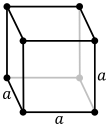
\includegraphics{Bravais_Cubic.png}
\caption{\small simple cubic cell.}%(与文献\cite{EPJB33-47_2003}图1对比)
\label{Bravais:Cubic}
\end{figure}
\begin{displaymath}
	\begin{aligned}
	& a=b=c &\alpha=\beta=\gamma=90^{\circ} \\
		&\mathrm{In\_Primitive\_cell}:&(1,0,0)\;(0,1,0)\;(0,0,1)\;\;\;\;\vec a=\vec A_1 \\
		& &\cos(\angle\vec A_1\vec A_2)=\cos(\angle\vec A_2\vec A_3)=\cos(\angle\vec A_3\vec A_1)=0
	\end{aligned}
\end{displaymath}
		\item 体心立方(\textrm{body-centered cubic cell})
\begin{figure}[h!]
\centering
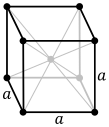
\includegraphics{Bravais_Cubic-body-centered.png}
\caption{\small body-centered cubic cell.}%(与文献\cite{EPJB33-47_2003}图1对比)
\label{Bravais:body-centered Cubic}
\end{figure}
\begin{displaymath}
	\begin{aligned}
		& a=b=c &\alpha=\beta=\gamma=90^{\circ} \\
		&\mathrm{In\_Primitive\_cell}: &(-\frac12,\frac12\frac12)\;(\frac12,-\frac12,\frac12)\;(\frac12,\frac12,-\frac12)\;\;\;\;&\vec a=\frac2{\sqrt 3}\vec A_1\\
		& &\cos(\angle\vec A_1\vec A_2)=\cos(\angle\vec A_2\vec A_3)=\cos(\angle\vec A_3\vec A_1)=-\frac13
	\end{aligned}
\end{displaymath}
		\item 面心立方(\textrm{face-centered cubic cell})
\begin{figure}[h!]
\centering
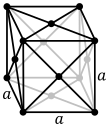
\includegraphics{Bravais_Cubic-face-centered.png}
\caption{\small face-centered cubic cell.}%(与文献\cite{EPJB33-47_2003}图1对比)
\label{Bravais:face-centered Cubic}
\end{figure}
\begin{displaymath}
	\begin{aligned}
	& a=b=c\qquad &\alpha=\beta=\gamma=90^{\circ}\\
		&\mathrm{In\_Primitive\_cell}:&(0,\frac12,\frac12)\;(\frac12,0,\frac12)\;(\frac12,\frac12,0)\;\;\;\;&\vec a=\sqrt 2\vec A_1\\
		& &\cos(\angle\vec A_1\vec A_2)=\cos(\angle\vec A_2\vec A_3)=\cos(\angle\vec A_3\vec A_1)=\frac12
	\end{aligned}
\end{displaymath}
		\item 六方(\textrm{hexagonal cell})
\begin{figure}[h!]
\centering
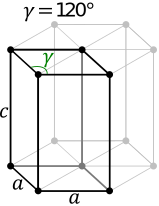
\includegraphics{Bravais_Hexagonal_latticeFRONT.png}
\caption{\small hexagonal cell.}%(与文献\cite{EPJB33-47_2003}图1对比)
\label{Bravais:hexagonal cell}
\end{figure}
\begin{displaymath}
	\begin{aligned}
		& a=b\neq c & \alpha=\beta=90^{\circ} \quad \gamma=120^{\circ}\\
		&\mathrm{In\_Primitive\_cell}:&(\sin120^{\circ},\cos120^{\circ},0)\;(0,1,0)\;(0,0,\frac{c}{a})\;\;\;\;&\vec a=\vec A_1\\
		& &\cos(\angle\vec A_1\vec A_2)=-\frac12\quad\cos(\angle\vec A_2\vec A_3)=\cos(\angle\vec A_3\vec A_1)=0
	\end{aligned}
\end{displaymath}
		\item 简单四方(\textrm{simple tetragonal cell})
\begin{figure}[h!]
\centering
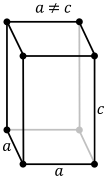
\includegraphics{Bravais_Tetragonal.png}
\caption{\small simple tetragonal cell.}%(与文献\cite{EPJB33-47_2003}图1对比)
\label{Bravais:tetragonal cell}
\end{figure}
\begin{displaymath}
	\begin{aligned}
	&a=b\neq c &\alpha=\beta=\gamma=90^{\circ} \\
	&\mathrm{In\_Primitive\_cell}:&(1,0,0)\;(0,1,0)\;(0,0,\frac{c}{a})\;\;\;\;\vec a=\vec A_1\\
		& &\cos(\angle\vec A_1\vec A_2)=\cos(\angle\vec A_2\vec A_3)=\cos(\angle\vec A_3\vec A_1)=0
	\end{aligned}
\end{displaymath}
		\item 体心四方(\textrm{body-centered tetragonal cell})
\begin{figure}[h!]
\centering
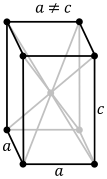
\includegraphics{Bravais_Tetragonal-body-centered.png}
\caption{\small tetragonal-body-centered cell.}%(与文献\cite{EPJB33-47_2003}图1对比)
\label{Bravais:tetragonal-body-centered}
\end{figure}
\begin{displaymath}
	\begin{aligned}
	&a=b\neq c & \alpha=\beta=\gamma=90^{\circ} \\
	&\mathrm{In\_Primitive\_cell}:&(-\frac12,\frac12,\frac{c}{2a})\;(\frac12,-\frac12,\frac{c}{2a})\;(\frac12,\frac12,\frac{c}{2a})\\
	& &\vec A_1=\vec A_2=\vec A_3\quad (\vec A_1+\vec A_2)\perp(\vec A_1+\vec A_3)\perp(\vec A_2+\vec A_3)\\
	& &|\vec A_1+\vec A_2|=|\vec A_2+\vec A_3|<|\vec A_1+\vec A_2|\\
		& &\cos(\angle\vec A_1\vec A_2)=\cos(\angle\vec A_2\vec A_3)\neq0\cos(\angle\vec A_3\vec A_1)\neq0
	\end{aligned}
\end{displaymath}
		\item 三方(\textrm{rhombohedral (trigonal) cell})
\begin{figure}[h!]
\centering
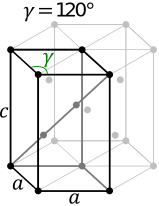
\includegraphics{Bravais_Hexagonal_latticeR.png}
\caption{\small rhombohedral (trigonal) cell.}%(与文献\cite{EPJB33-47_2003}图1对比)
\label{Bravais:rhombohedral cell}
\end{figure}
\begin{displaymath}
	\begin{aligned}
	& a=b=c &\alpha=\beta=\gamma\neq90^{\circ}\\
	&\mathrm{In\_Primitive\_cell}:~&(0,\eta,\zeta)\;(-\frac{\sqrt3\eta}2,-\frac{\eta}2,\zeta)\;(\frac{\sqrt3\eta}2,-\frac{\eta}2,\zeta)\;\;\;\;\vec a=\vec A_1\\
	&&\zeta=\sqrt{\frac{2\cos\alpha+1}3}\qquad \eta=\sqrt{\frac{2(1-\cos\alpha)}3}\\
		& & \cos(\angle\vec A_1\vec A_2)=\cos(\angle\vec A_2\vec A_3)=\cos(\angle\vec A_3\vec A_1)\neq 0
	\end{aligned}
\end{displaymath}
		\item 简单正交(\textrm{simple orthorhombic cell})
\begin{figure}[h!]
\centering
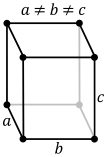
\includegraphics{Bravais_Orthorhombic.png}
\caption{\small simple orthorhombic cell.}%(与文献\cite{EPJB33-47_2003}图1对比)
\label{Bravais:orthorhombic cell}
\end{figure}
\begin{displaymath}
	\begin{aligned}
	&a\neq b\neq c &\alpha=\beta=\gamma=90^{\circ} \\
	&\mathrm{In\_Primitive\_cell}:~&(1,0,0)\;(0,\frac{b}{a},0)\;(0,0,\frac{c}{a})\\
		& &\cos(\angle\vec A_1\vec A_2)=\cos(\angle\vec A_2\vec A_3)=\cos(\angle\vec A_3\vec A_1)=0
	\end{aligned}
\end{displaymath}
		\item 体心正交(\textrm{body-centered orthorhombic cell})
\begin{figure}[h!]
\centering
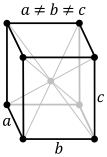
\includegraphics{Bravais_Orthorhombic-body-centered.png}
\caption{\small body-centered orthorhombic.}%(与文献\cite{EPJB33-47_2003}图1对比)
\label{Bravais:orthorhombic-body-centered}
\end{figure}
\begin{displaymath}
	\begin{aligned}
	&a\neq b\neq c &\alpha=\beta=\gamma=90^{\circ} \\
	&\mathrm{In\_Primitive\_cell}:~&(-\frac12,\frac{b}{2a},\frac{c}{2a})\;(\frac12,-\frac{b}{2a},\frac{c}{2a})\;(\frac12,\frac{b}{2a},-\frac{c}{2a})\\
	& &\vec A_1=\vec A_2=\vec A_3\quad (\vec A_1+\vec A_2)\perp(\vec A_1+\vec A_3)\perp(\vec A_2+\vec A_3)\\ 
	& &|\vec A_1+\vec A_2|>|\vec A_1+\vec A_3|>|\vec A_2+\vec A_3|\\
		& &\cos(\angle\vec A_1\vec A_2)\neq\cos(\angle\vec A_2\vec A_3)\neq\cos(\angle\vec A_3\vec A_1)\neq0
	\end{aligned}
\end{displaymath}
		\item 面心正交(\textrm{face-centered orthorhombic cell})
\begin{figure}[h!]
\centering
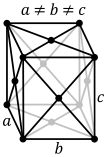
\includegraphics{Bravais_Orthorhombic-face-centered.png}
\caption{\small face-centered orthorhombic.}%(与文献\cite{EPJB33-47_2003}图1对比)
\label{Bravais:orthorhombic-face-centered}
\end{figure}
\begin{displaymath}
	\begin{aligned}
	&a\neq b\neq c &\alpha=\beta=\gamma=90^{\circ} \\
	&\mathrm{In\_Primitive\_cell}:~&(0,\frac{b}{2a},\frac{c}{2a})\;(\frac12,0,\frac{c}{2a})\;(\frac12,\frac{b}{2a},0)\\
	& & |\vec A_1|=|\vec A_2-\vec A_3|\;|\vec A_2|=|\vec A_1-\vec A_3|\;|\vec A_3|=|\vec A_1-\vec A_2|\\
	& &|\vec A_1+\vec A_2-\vec A_3|>|\vec A_1+\vec A_3-\vec A_2|>|\vec A_2+\vec A_3-\vec A_1|\\
		& &\cos(\angle\vec A_1\vec A_2)\neq\cos(\angle\vec A_2\vec A_3)\neq\cos(\angle\vec A_3\vec A_1)\neq0
	\end{aligned}
\end{displaymath}
		\item 底心正交(\textrm{base-centered orthorhombic cell})
\begin{figure}[h!]
\centering
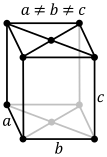
\includegraphics{Bravais_Orthorhombic-base-centered.png}
\caption{\small base-centered orthorhombic.}%(与文献\cite{EPJB33-47_2003}图1对比)
\label{Bravais:orthorhombic-base-centered}
\end{figure}
\begin{displaymath}
	\begin{aligned}
		&a\neq b\neq c &\alpha=\beta=90^{\circ}\quad\gamma\neq90^{\circ} \\
	&\mathrm{In\_Primitive\_cell}:~&(\frac12,-\frac{b}{2a},0)\;(\frac12,\frac{b}{2a},0)\;(0,0,\frac{c}{a})\;\;\;\;\vec A_1=\vec A_2\neq\vec A_3\\
		& &\cos(\angle\vec A_2\vec A_3)=\cos(\angle\vec A_3\vec A_1)=0\quad\cos(\angle\vec A_1\vec A_2)<0
	\end{aligned}
\end{displaymath}
		\item 简单单斜(\textrm{simple monoclinic cell})
\begin{figure}[h!]
\centering
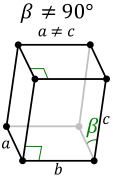
\includegraphics{Bravais_Monoclinic.png}
\caption{\small simple Monoclinic cell.}%(与文献\cite{EPJB33-47_2003}图1对比)
\label{Bravais:monoclinic}
\end{figure}
\begin{displaymath}
	\begin{aligned}
		&a\neq b\neq c &\alpha=\gamma=90^{\circ}\quad\beta\neq90^{\circ} \\
	&\mathrm{In\_Primitive\_cell}:~&(\sin\beta,0,-\cos\beta)\;(0,\frac{b}{a},0)\;(0,0,\frac{c}{a})\\
		& &\cos(\angle\vec A_2\vec A_3)=\cos(\angle\vec A_3\vec A_1)=0\qquad\cos(\angle\vec A_1\vec A_2)<0
	\end{aligned}
\end{displaymath}
		\item 底心单斜(\textrm{base-centered monoclinic cell})
\begin{figure}[h!]
\centering
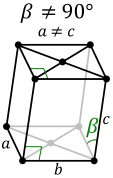
\includegraphics{Bravais_Monoclinic-base-centered.png}
\caption{\small base-centered monoclinic.}%(与文献\cite{EPJB33-47_2003}图1对比)
\label{Bravais:base-centered monoclinic}
\end{figure}
\begin{displaymath}
	\begin{aligned}
		&a\neq b\neq c &\alpha=\gamma=90^{\circ}\quad\beta\neq90^{\circ} \\
		&\mathrm{In\_Primitive\_cell}:~&(\frac12,-\frac{b}{2a},0)\;(\frac12,\frac{b}{2a},0)\;(\frac{c\cos\beta}{a},0,\frac{c\sin\beta}{a})\;\;\;\;\vec A_1=\vec A_2\neq\vec A_3\\
		& &\cos(\angle\vec A_1\vec A_2)=0\;\cos(\angle\vec A_3\vec A_2)<0\;\cos(\angle\vec A_3\vec A_1)<0
	\end{aligned}
\end{displaymath}
		\item 三斜(\textrm{triclinic})
\begin{figure}[h!]
\centering
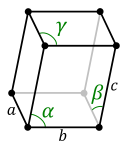
\includegraphics{Bravais_Triclinic.png}
\caption{\small triclinic cell.}%(与文献\cite{EPJB33-47_2003}图1对比)
\label{Bravais:triclinic}
\end{figure}
\begin{displaymath}
	\begin{aligned}
	& a\neq b\neq c &\alpha\neq\beta\neq\gamma\\
	&\mathrm{In\_Primitive\_cell}:~&(\sin\beta,0,\cos\beta)\;(a_2x,a_2y,a_2z)\;(0,0,\frac{c}{a})\\
	& &a_2x=\frac{b}{a}\frac{(\cos\gamma-\cos\alpha\cos\beta)}{\sin\beta}\\
	& &a_2y=\sqrt{\left( \frac{b}{a} \right)^2\sin^2\alpha-(a_2x)^2}\\
	& &a_2z=\frac{b}{a}\cos\beta \\
		& &\cos(\angle\vec A_1\vec A_2)\neq\cos(\angle\vec A_2\vec A_3)\neq\cos(\angle\vec A_3\vec A_1)\neq0
	\end{aligned}
\end{displaymath}
\end{enumerate}

\section{附录2:~\rm{Bravais~vector}和坐标变换关系}
在计算程序中,采用\textrm{Bravais matrix~}表示的晶胞,其坐标称为\textrm{Direct~}坐标和\textrm{Reciprocal}坐标,其与\textrm{Cartesian~}坐标的关系是
\begin{displaymath}
	\vec k=x_1\vec b_1+x_2\vec b_2+x_3\vec b_3=\frac{2\pi}a(x_1^{\prime},x_2^{\prime},x_3^{\prime})
\end{displaymath}
以面心立方(\textbf{FCC})为例:~\\
\textrm{Diract lattice~}定义为
\begin{displaymath}
	\mathbf{A}=\left(
	\begin{matrix}
		0 &a/2 &a/2\\
		a/2 &0 &a/2\\
		a/2 &a/2 &0
	\end{matrix}\right)
\end{displaymath}
对应的\textrm{Reciprocal lattice~}(\textcolor{red}{\textrm{FCC~}面心立方的倒格子是\textrm{BCC~}格子,见图\ref{Fig:primitive_reciprocal}})定义为
\begin{figure}[h!]
\centering
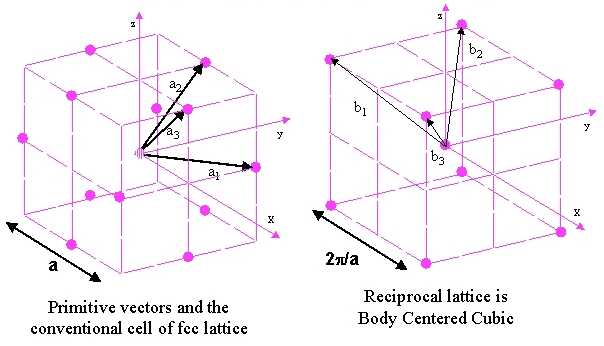
\includegraphics{Direct-Reciprocal_vector-FCC.png}
\caption{\small The relation of the primitive vector and the reciprocal vector.}%(与文献\cite{EPJB33-47_2003}图1对比)
\label{Fig:primitive_reciprocal}
\end{figure}

\begin{displaymath}
	\mathbf{B}=\frac{2\pi}a\left(
	\begin{matrix}
		-1 &1 &1\\
		1 &-1 &1\\
		1 &1 &-1
	\end{matrix}\right)
\end{displaymath}
\begin{table}[!h]
\tabcolsep 0pt \vspace*{-12pt}
%\caption{The representative $\vec k$ points contributing to $\sigma_2^{xy}$ of interband transition in EuTe around 2.5 eV.}
\label{Table-coordinate}
%\begin{center}
\centering
\def\temptablewidth{0.84\textwidth}
\rule{\temptablewidth}{1pt}
\begin{tabular*} {\temptablewidth}{@{\extracolsep{\fill}}c@{\extracolsep{\fill}}c@{\extracolsep{\fill}}c}

%-------------------------------------------------------------------------------------------------------------------------
	\textrm{Point} & \textrm{Cartesian coordinates} &\textrm{Reciprocal coordinates} \\
	&\textrm{(unit of 2$\pi$/a)} &\textrm{(unit of $\vec b_1$,$\vec b_2$,$\vec b_3$)}\\\hline
	\textbf{G} &(0, 0, 0) &(0, 0, 0)\\
	\textbf{X} &(0, 0, 1) &(1/2, 1/2, 0)\\
	\textbf{W} &(1/2, 0, 1) &(1/2, 3/4, 1/4)\\
	\textbf{K} &(3/4, 3/4, 0) &(3/8, 3/8, 3/4)\\
	\textbf{L} &(1/2, 1/2, 1/2) &(1/2, 1/2, 1/2)\\
%-------------------------------------------------------------------------------------------------------------------------
%-------------------------------------------------------------------------------------------------------------------------
\end{tabular*}
\rule{\temptablewidth}{1pt}
\end{table}
以\textbf{X}~点为例:
\begin{displaymath}
	\begin{aligned}
		&\textcolor{red}{\frac12}\cdot\vec b_1+\textcolor{red}{\frac12}\cdot\vec b_2+\textcolor{red}{0}\cdot\vec b_3\\
		=&\textcolor{red}{\frac12}\cdot\textcolor{blue}{(-1, 1, 1)}\cdot\frac{2\pi}a+\textcolor{red}{\frac12}\cdot\textcolor{blue}{(1, -1, 1)}\cdot\frac{2\pi}a+\textcolor{red}{0}\cdot\textcolor{blue}{(1, 1, -1)}\cdot\frac{2\pi}a\\
		=&(\frac12\cdot(-1)+\frac12\cdot1+0\cdot1,\frac12\cdot1+\frac12\cdot(-1)+0\cdot1,\frac12\cdot1+\frac12\cdot1+0\cdot1)\cdot\frac{2\pi}a\\
		=&(-\frac12+\frac12+0,\frac12-\frac12+0,\frac12+\frac12+0)\cdot\frac{2\pi}a\\
		=&\textcolor{magenta}{(0,0,1)}\cdot\frac{2\pi}a
	\end{aligned}
\end{displaymath}
以\textbf{W}~点为例:
\begin{displaymath}
	\begin{aligned}
		&\textcolor{red}{\frac12}\cdot\vec b_1+\textcolor{red}{\frac34}\cdot\vec b_2+\textcolor{red}{\frac14}\cdot\vec b_3\\
		=&\textcolor{red}{\frac12}\cdot\textcolor{blue}{(-1, 1, 1)}\cdot\frac{2\pi}a+\textcolor{red}{\frac34}\cdot\textcolor{blue}{(1, -1, 1)}\cdot\frac{2\pi}a+\textcolor{red}{\frac14}\cdot\textcolor{blue}{(1, 1, -1)}\cdot\frac{2\pi}a\\
		=&(\frac12\cdot(-1)+\frac12\cdot1+0\cdot1,\frac34\cdot1+\frac34\cdot(-1)+\frac14\cdot1,\frac12\cdot1+\frac34\cdot1+\frac14\cdot1)\cdot\frac{2\pi}a\\
		=&(-\frac12+\frac34+\frac14,\frac12-\frac34+\frac14,\frac12+\frac34-\frac14)\cdot\frac{2\pi}a\\
		=&\textcolor{magenta}{(\frac12,0,1)}\cdot\frac{2\pi}a
	\end{aligned}
\end{displaymath}

\section{附录3:~点群和空间群的对应关系}
\begin{figure}[h!]
\centering
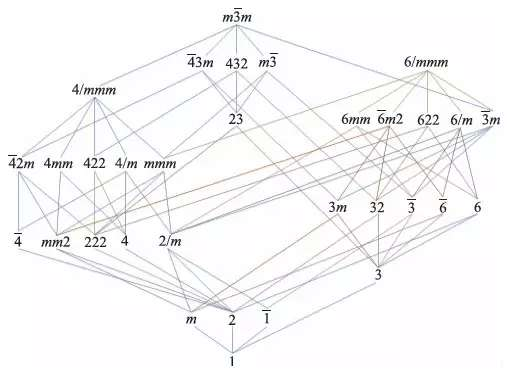
\includegraphics{Point_Group.jpg}
\caption{\small The relation of 32 point-group.}%(与文献\cite{EPJB33-47_2003}图1对比)
\label{Fig:Point_Group}
\end{figure}

\begin{small}
%\begin{minipage}{\textwidth}
%\begin{longtable}[l]{|c|c|cc|c|c|} %[c]指定长表格对齐方式
\begin{longtable}[c]{|c|c|c|c|c|c|c|c|c|}
	\caption{\textrm{The 32 Point-Group and 230 Space-Group}}
\label{tab:Space-Group}\\ %\\长表格的caption中换行不可少
\hline
%
%--------------------------------------------------------------------------------------------------------------------------------
&\multicolumn{4}{c|}{\textrm{Point-Group}}  &\multicolumn{4}{c|}{\textrm{Space-Group}} \\ \cline{2-9}
\raisebox{2.3ex}[0pt][0pt]{\textrm{Crystal}:} &\textrm{No.}  & \multicolumn{2}{c}{} & &\textrm{No.} &$\mathrm{N}_{\mathbf{Tr}}$ & \multicolumn{2}{c|}{\textrm{Bravais-Latt}:}\\ \hline
\endfirsthead
%--------------------------------------------------------------------------------------------------------------------------------
%
\multicolumn{10}{r}{\it 续表}\\
\hline
%--------------------------------------------------------------------------------------------------------------------------------
&\multicolumn{4}{c|}{\textrm{Point-Group}}  &\multicolumn{4}{c|}{\textrm{Space-Group}} \\ \cline{2-9}
\raisebox{2.3ex}[0pt][0pt]{\textrm{Crystal}:} &\textrm{No.}  &\multicolumn{2}{c}{} & &\textrm{No.} &$\mathrm{N}_{\mathbf{Tr}}$ & \multicolumn{2}{c|}{\textrm{Bravais-Latt}:}\\ \hline
\endhead
%--------------------------------------------------------------------------------------------------------------------------------
%
\multicolumn{10}{r}{\it 续下页}\\
\endfoot
\hline
%--------------------------------------------------------------------------------------------------------------------------------
%
%\hlinewd{0.5$p$t}
\endlastfoot
%--------------------------------------------------------------------------------------------------------------------------------
%
% Stuff from here to \endlastfoot goes at bottom of last page.
%
%--------------------------------------------------------------------------------------------------------------------------------
& \textrm{01} &\textbf{1} &\textbf{1} &$\mathbf{C}_1$ &\textrm{1} &0 &\textbf{P1}&\textbf{P1} \\\cline{2-9}
\raisebox{2.3ex}[0pt][0pt]{\textrm{Triclinic}} & \textrm{02} &\textbf{-1} &\textbf{-1} &$\mathbf{S}_2$ &\textrm{2} &0 &\textbf{P-1}&\textbf{-P1} \\\hline
%--------------------------------------------------------------------------------------------------------------------------------
 & & & & & & & &\textbf{P2\textcolor{red}{x}}  \\\cline{9-9}
 & & & & &\textrm{3} &0 &\textbf{P2}&\textbf{P2\textcolor{red}{y}} \\\cline{9-9}
 & & & & & & & &\textbf{P2\textcolor{red}{z}}  \\\cline{6-9}
 & & & & & & & &\textbf{P2\textcolor{red}{xa}}  \\\cline{9-9}
 & & & & &\textrm{4} &1 &\textbf{P21}&\textbf{P2\textcolor{red}{yb}} \\\cline{9-9}
 & & & & & & & &\textbf{P2\textcolor{red}{zc}}  \\\cline{6-9}
 & \textrm{03} &\textbf{2} &\textbf{2} &$\mathbf{C}_2$ & & &\textbf{C2}&\textbf{C2\textcolor{red}{x}} \\\cline{8-9}
 & & & & & & &\textbf{A2} &\textbf{A2\textcolor{red}{y}}  \\\cline{8-9}
 & & & & & & &\textbf{B2} &\textbf{B2\textcolor{red}{z}}  \\\cline{8-9}
 & & & & &\textrm{5} &2&\textbf{B2} &\textbf{B2\textcolor{red}{x}}  \\\cline{8-9}
 & & & & & & &\textbf{C2} &\textbf{C2\textcolor{red}{y}}  \\\cline{8-9}
 & & & & & & &\textbf{A2} &\textbf{A2\textcolor{red}{z}}  \\\cline{2-9}
%--------------------------------------------------------------------------------------------------------------------------------
 & & & & & & & &\textbf{P-2\textcolor{red}{x}}  \\\cline{9-9}
 & & & & &\textrm{6} &0 &\textbf{Pm}&\textbf{P-2\textcolor{red}{y}} \\\cline{9-9}
 & & & & & & & &\textbf{P-2\textcolor{red}{z}}  \\\cline{6-9}
 & & & & & & &\textbf{Pc} &\textbf{P-2\textcolor{red}{xc}}  \\\cline{8-9}
 & & & & & & &\textbf{Pa} &\textbf{P-2\textcolor{red}{ya}}  \\\cline{8-9}
 & & & & & & &\textbf{Pb} &\textbf{P-2\textcolor{red}{zb}}  \\\cline{8-9}
 & & & & &\textrm{7} &1&\textbf{Pb} &\textbf{P-2\textcolor{red}{xb}}  \\\cline{8-9}
 & & & & & & &\textbf{Pc} &\textbf{P-2\textcolor{red}{yc}}  \\\cline{8-9}
 & & & & & & &\textbf{Pa} &\textbf{P-2\textcolor{red}{za}}  \\\cline{8-9}
 & & & & & & & &\textbf{P-2\textcolor{red}{xbc}}  \\\cline{9-9}
 & & & & & & &\textbf{Pn} &\textbf{P-2\textcolor{red}{yac}}  \\\cline{9-9}
 & & & & & & & &\textbf{P-2\textcolor{red}{zab}}  \\\cline{6-9}
 & \textrm{04} &\textbf{m} &\textbf{m} &$\mathbf{C}_s$ & & &\textbf{Cm}&\textbf{C-2\textcolor{red}{x}} \\\cline{9-9}
 & & & & & & &\textbf{Am} &\textbf{A-2\textcolor{red}{y}}  \\\cline{8-9}
 & & & & & & &\textbf{Bm} &\textbf{P-2\textcolor{red}{z}}  \\\cline{8-9}
 & & & & &\textrm{8} &2&\textbf{Bm} &\textbf{B-2\textcolor{red}{x}}  \\\cline{8-9}
 & & & & & & &\textbf{Cm} &\textbf{C-2\textcolor{red}{y}}  \\\cline{8-9}
 & & & & & & &\textbf{Am} &\textbf{A-2\textcolor{red}{z}}  \\\cline{6-9}
\textrm{Monoclinic} & & & & & & &\textbf{Am} &\textbf{A-2\textcolor{red}{z}}  \\\cline{8-9}
 & & & & & & &\textbf{Cc} &\textbf{C-2\textcolor{red}{xa}}  \\\cline{8-9}
 & & & & & & &\textbf{Aa} &\textbf{A-2\textcolor{red}{ya}}  \\\cline{8-9}
 & & & & &\textrm{9} &3&\textbf{Bb} &\textbf{B-2\textcolor{red}{xb}}  \\\cline{8-9}
 & & & & & & &\textbf{Cc} &\textbf{C-2\textcolor{red}{yc}}  \\\cline{8-9}
 & & & & & & &\textbf{Aa} &\textbf{A-2\textcolor{red}{za}}  \\\cline{2-9}
%--------------------------------------------------------------------------------------------------------------------------------
 & & & & & & & &\textbf{-P2\textcolor{red}{x}}  \\\cline{9-9}
 & & & & &\textrm{10} &0 &\textbf{P2/m}&\textbf{-P2\textcolor{red}{y}} \\\cline{9-9}
 & & & & & & & &\textbf{-P2\textcolor{red}{z}}  \\\cline{6-9}
 & & & & & & & &\textbf{-P2\textcolor{red}{xa}}  \\\cline{9-9}
 & & & & &\textrm{11} &1 &\textbf{P21/m}&\textbf{-P2\textcolor{red}{yb}} \\\cline{9-9}
 & & & & & & & &\textbf{-P2\textcolor{red}{zc}}  \\\cline{6-9}
 & & & & & & &\textbf{C2/m} &\textbf{-C2\textcolor{red}{x}}  \\\cline{8-9}
 & & & & & & &\textbf{A2/m} &\textbf{-A2\textcolor{red}{y}}  \\\cline{8-9}
 & & & & & & &\textbf{B2/m} &\textbf{-B2\textcolor{red}{z}}  \\\cline{8-9}
 & & & & &\textrm{12} &2&\textbf{B2/m} &\textbf{-B2\textcolor{red}{x}}  \\\cline{8-9}
 & & & & & & &\textbf{C2/m} &\textbf{-C2\textcolor{red}{y}}  \\\cline{8-9}
 & & & & & & &\textbf{A2/m} &\textbf{-A2\textcolor{red}{z}}  \\\cline{6-9}
 & & & & & & &\textbf{P2/c} &\textbf{-P2\textcolor{red}{xc}}  \\\cline{8-9}
 & & & & & & &\textbf{P2/a} &\textbf{-P2\textcolor{red}{ya}}  \\\cline{8-9}
 & & & & & & &\textbf{P2/b} &\textbf{-P2\textcolor{red}{zb}}  \\\cline{8-9}
 & & & & & & &\textbf{P2/b} &\textbf{-P2\textcolor{red}{xb}}  \\\cline{8-9}
 & \textrm{05} &\textbf{2/m} &\textbf{2/m} &$\mathbf{C}_{2h}$ &\textrm{13} &3 &\textbf{P2/c}&\textbf{-P2\textcolor{red}{yc}} \\\cline{8-9}
 & & & & & & &\textbf{P2/a} &\textbf{-P2\textcolor{red}{za}}  \\\cline{8-9}
 & & & & & & & &\textbf{-P2\textcolor{red}{xbc}}  \\\cline{9-9}
 & & & & & & &\textbf{P2/n} &\textbf{-P2\textcolor{red}{yac}}  \\\cline{9-9}
 & & & & & & & &\textbf{-P2\textcolor{red}{zab}}  \\\cline{6-9}
 & & & & & & &\textbf{P21/c} &\textbf{-P2\textcolor{red}{xca}}  \\\cline{8-9}
 & & & & & & &\textbf{P21/a} &\textbf{-P2\textcolor{red}{yab}}  \\\cline{8-9}
 & & & & & & &\textbf{P21/b} &\textbf{-P2\textcolor{red}{zbc}}  \\\cline{8-9}
 & & & & & & &\textbf{P21/b} &\textbf{-P2\textcolor{red}{xba}}  \\\cline{8-9}
 & & & & &\textrm{14} &4 &\textbf{P21/c}&\textbf{-P2\textcolor{red}{ycb}} \\\cline{8-9}
 & & & & & & &\textbf{P21/a} &\textbf{-P2\textcolor{red}{zac}}  \\\cline{8-9}
 & & & & & & & &\textbf{-P2\textcolor{red}{xabc}}  \\\cline{9-9}
 & & & & & & &\textbf{P21/n} &\textbf{-P2\textcolor{red}{yabc}}  \\\cline{9-9}
 & & & & & & & &\textbf{-P2\textcolor{red}{zabc}}  \\\cline{6-9}
 & & & & & & &\textbf{C2/c} &\textbf{-C2\textcolor{red}{xc}}  \\\cline{8-9}
 & & & & & & &\textbf{A2/a} &\textbf{-A2\textcolor{red}{ya}}  \\\cline{8-9}
 & & & & & & &\textbf{B2/b} &\textbf{-B2\textcolor{red}{zb}}  \\\cline{8-9}
 & & & & &\textrm{15} &5 &\textbf{B2/b} &\textbf{-B2\textcolor{red}{xb}}  \\\cline{8-9}
 & & & & & & &\textbf{C2/c} &\textbf{-C2\textcolor{red}{yc}}  \\\cline{8-9}
 & & & & & & &\textbf{A2/a} &\textbf{-A2\textcolor{red}{za}}  \\\hline
%--------------------------------------------------------------------------------------------------------------------------------
 & & & & &\textrm{16} &0 &\textbf{P222} &\textbf{P2\textcolor{red}{z};2\textcolor{red}{x}}  \\\cline{6-9}
 & & & & & & &\textbf{P2221} &\textbf{P2\textcolor{red}{zc};2\textcolor{red}{x}}  \\\cline{8-9}
 & & & & &\textrm{17} &1 &\textbf{P2122} &\textbf{P2\textcolor{red}{xa};2\textcolor{red}{y}}  \\\cline{8-9}
 & & & & & & &\textbf{P2212} &\textbf{P2\textcolor{red}{yb};2\textcolor{red}{z}}  \\\cline{6-9}
 & & & & & & &\textbf{P21212} &\textbf{P2\textcolor{red}{z};2\textcolor{red}{xab}}  \\\cline{8-9}
 & & & & &\textrm{18} &2 &\textbf{P22121} &\textbf{P2\textcolor{red}{x};2\textcolor{red}{ybc}}  \\\cline{8-9}
 & & & & & & &\textbf{P21221} &\textbf{P2\textcolor{red}{y};2\textcolor{red}{zca}}  \\\cline{6-9}
 & & & & &\textrm{19} &3 &\textbf{P212121} &\textbf{P2\textcolor{red}{zac};2\textcolor{red}{xab}}  \\\cline{6-9}
 & \textrm{06} & \textbf{222} & \textbf{222} & $\mathbf{D}_2$ & & &\textbf{C2221} &\textbf{C2\textcolor{red}{zc};2\textcolor{red}{x}}  \\\cline{8-9}
 & & & & &\textrm{20} &4 &\textbf{A2122} &\textbf{A2\textcolor{red}{xa};2\textcolor{red}{y}}  \\\cline{8-9}
 & & & & & & &\textbf{B2212} &\textbf{B2\textcolor{red}{yb};2\textcolor{red}{z}}  \\\cline{6-9}
 & & & & & & &\textbf{C222} &\textbf{C2\textcolor{red}{z};2\textcolor{red}{x}}  \\\cline{8-9}
 & & & & &\textrm{21} &5 &\textbf{A222} &\textbf{A2\textcolor{red}{x};2\textcolor{red}{y}}  \\\cline{8-9}
 & & & & & & &\textbf{B222} &\textbf{B2\textcolor{red}{y};2\textcolor{red}{z}}  \\\cline{6-9}
 & & & & &\textrm{22} &6 &\textbf{F222} &\textbf{F2\textcolor{red}{z};2\textcolor{red}{x}}  \\\cline{6-9}
 & & & & &\textrm{23} &7 &\textbf{I222} &\textbf{I2\textcolor{red}{z};2\textcolor{red}{x}}  \\\cline{6-9}
 & & & & &\textrm{24} &8 &\textbf{I212121} &\textbf{I2\textcolor{red}{zac};2\textcolor{red}{xab}}  \\\cline{
 2-9}
%--------------------------------------------------------------------------------------------------------------------------------
          &  & & & &  & &\textbf{Pmm2}         &\textbf{P2\textcolor{red}{z};-2\textcolor{red}{x}}\\\cline{8-9}           
	  &  & & & &\textrm{25}  &\textrm{0} &\textbf{P2mm}         &\textbf{P2\textcolor{red}{x};-2\textcolor{red}{y}}\\\cline{8-9}           
          &  & & & &  & &\textbf{Pm2m}         &\textbf{P2\textcolor{red}{y};-2\textcolor{red}{z}}\\\cline{6-9}           
          &  & & & &  & &\textbf{Pmc21}       &\textbf{P2\textcolor{red}{zc};-2\textcolor{red}{x}}\\\cline{8-9}          
          &  & & & &  & &\textbf{P21ma}       &\textbf{P2\textcolor{red}{xa};-2\textcolor{red}{y}}\\\cline{8-9}          
          &  & & & &  & &\textbf{Pb21m}       &\textbf{P2\textcolor{red}{yb};-2\textcolor{red}{z}}\\\cline{8-9}          
	  &  & & & &\textrm{26}  &\textrm{1} &\textbf{Pcm21}       &\textbf{P2\textcolor{red}{zc};-2\textcolor{red}{y}}\\\cline{8-9}          
          &  & & & &  & &\textbf{P21am}       &\textbf{P2\textcolor{red}{xa};-2\textcolor{red}{z}}\\\cline{8-9}        
          &  & & & &  & &\textbf{Pm21b}       &\textbf{P2\textcolor{red}{yb};-2\textcolor{red}{x}}\\\cline{6-9}          
          &  & & & &  & &\textbf{Pcc2}         &\textbf{P2\textcolor{red}{z};-2\textcolor{red}{xc}}\\\cline{8-9}          
	  &  & & & &\textrm{27}  &\textrm{2} &\textbf{P2aa}         &\textbf{P2\textcolor{red}{x};-2\textcolor{red}{ya}}\\\cline{8-9}          
          &  & & & &  & &\textbf{Pb2b}         &\textbf{P2\textcolor{red}{y};-2\textcolor{red}{zb}}\\\cline{6-9}          
          &  & & & &  & &\textbf{Pma2}         &\textbf{P2\textcolor{red}{z};-2\textcolor{red}{xa}}\\\cline{8-9}          
          &  & & & &  & &\textbf{P2mb}         &\textbf{P2\textcolor{red}{x};-2\textcolor{red}{yb}}\\\cline{8-9}          
          &  & & & &  & &\textbf{Pc2m}         &\textbf{P2\textcolor{red}{y};-2\textcolor{red}{zc}}\\\cline{8-9}          
	  &  & & & &\textrm{28}  &\textrm{3} &\textbf{Pbm2}         &\textbf{P2\textcolor{red}{z};-2\textcolor{red}{yb}}\\\cline{8-9}          
          &  & & & &  & &\textbf{P2cm}         &\textbf{P2\textcolor{red}{x};-2\textcolor{red}{zc}}\\\cline{8-9}          
          &  & & & &  & &\textbf{Pm2a}         &\textbf{P2\textcolor{red}{y};-2\textcolor{red}{xa}}\\\cline{6-9}        
          &  & & & &  & &\textbf{Pca21}       &\textbf{P2\textcolor{red}{zc};-2\textcolor{red}{xac}}\\\cline{8-9}        
          &  & & & &  & &\textbf{P21ab}       &\textbf{P2\textcolor{red}{xa};-2\textcolor{red}{yba}}\\\cline{8-9}        
          &  & & & &  & &\textbf{Pc21b}       &\textbf{P2\textcolor{red}{yb};-2\textcolor{red}{zcb}}\\\cline{8-9}        
	  &  & & & &\textrm{29}  &\textrm{4} &\textbf{Pbc21}       &\textbf{P2\textcolor{red}{zc};-2\textcolor{red}{ybc}}\\\cline{8-9}        
          &  & & & &  & &\textbf{P21ca}       &\textbf{P2\textcolor{red}{xa};-2\textcolor{red}{zca}}\\\cline{8-9}        
          &  & & & &  & &\textbf{Pb21a}       &\textbf{P2\textcolor{red}{yb};-2\textcolor{red}{xab}}\\\cline{6-9}        
          &  & & & &  & &\textbf{Pnc2}         &\textbf{P2\textcolor{red}{z};-2\textcolor{red}{xbc}}\\\cline{8-9}         
          &  & & & &  & &\textbf{P2na}         &\textbf{P2\textcolor{red}{x};-2\textcolor{red}{yca}}\\\cline{8-9}         
          &  & & & &  & &\textbf{Pb2n}         &\textbf{P2\textcolor{red}{y};-2\textcolor{red}{zab}}\\\cline{8-9}         
	  &  & & & &\textrm{30}  &\textrm{5} &\textbf{Pcn2}         &\textbf{P2\textcolor{red}{z};-2\textcolor{red}{yac}}\\\cline{8-9}         
          &  & & & &  & &\textbf{P2an}         &\textbf{P2\textcolor{red}{x};-2\textcolor{red}{zba}}\\\cline{8-9}         
          &  & & & &  & &\textbf{Pn2b}         &\textbf{P2\textcolor{red}{y};-2\textcolor{red}{xcb}}\\\cline{6-9}         
          &  & & & &  & &\textbf{Pmn21}       &\textbf{P2\textcolor{red}{zac};-2\textcolor{red}{x}}\\\cline{8-9}         
          &  & & & &  & &\textbf{P21mn}       &\textbf{P2\textcolor{red}{xba};-2\textcolor{red}{y}}\\\cline{8-9}         
          &  & & & &  & &\textbf{Pn21m}       &\textbf{P2\textcolor{red}{ycb};-2\textcolor{red}{z}}\\\cline{8-9}         
	  &  & & & &\textrm{31}  &\textrm{6} &\textbf{Pnm21}       &\textbf{P2\textcolor{red}{zbc};-2\textcolor{red}{y}}\\\cline{8-9}         
          &  & & & &  & &\textbf{P21nm}       &\textbf{P2\textcolor{red}{zca};-2\textcolor{red}{z}}\\\cline{8-9}         
          &  & & & &  & &\textbf{Pm21n}       &\textbf{P2\textcolor{red}{yab};-2\textcolor{red}{x}}\\\cline{6-9}         
          &  & & & &  & &\textbf{Pba2}         &\textbf{P2\textcolor{red}{z};-2\textcolor{red}{xab}}\\\cline{8-9}         
	  &  & & & &\textrm{32}  &\textrm{7} &\textbf{P2cb}         &\textbf{P2\textcolor{red}{x};-2\textcolor{red}{ybc}}\\\cline{8-9}         
          &  & & & &  & &\textbf{Pc2a}         &\textbf{P2\textcolor{red}{y};-2\textcolor{red}{zca}}\\\cline{6-9}         
          &  & & & &  & &\textbf{Pna21}       &\textbf{P2\textcolor{red}{zc};-2\textcolor{red}{xn}}\\\cline{8-9}         
          &  & & & &  & &\textbf{P21nb}       &\textbf{P2\textcolor{red}{xa};-2\textcolor{red}{yn}}\\\cline{8-9}         
          &  & & & &  & &\textbf{Pc21n}       &\textbf{P2\textcolor{red}{yb};-2\textcolor{red}{zn}}\\\cline{8-9}         
	  &  & & & &\textrm{33}  &\textrm{8} &\textbf{Pbn21}       &\textbf{P2\textcolor{red}{zc};-2\textcolor{red}{yn}}\\\cline{8-9}         
          &  & & & &  & &\textbf{P21cn}       &\textbf{P2\textcolor{red}{xa};-2\textcolor{red}{zn}}\\\cline{8-9}         
          &  & & & &  & &\textbf{Pn21a}       &\textbf{P2\textcolor{red}{yb};-2\textcolor{red}{xn}}\\\cline{6-9}         
          &  & & & &  & &\textbf{Pnn2}         &\textbf{P2\textcolor{red}{z};-2\textcolor{red}{xn}}\\\cline{8-9}          
	  &  & & & &\textrm{34}  &\textrm{9} &\textbf{P2nn}         &\textbf{P2\textcolor{red}{x};-2\textcolor{red}{yn}}\\\cline{8-9}          
          &  & & & &  & &\textbf{Pn2n}         &\textbf{P2\textcolor{red}{y};-2\textcolor{red}{zn}}\\\cline{6-9}          
          &  & & & &  & &\textbf{Cmm2}         &\textbf{C2\textcolor{red}{z};-2\textcolor{red}{x}}\\\cline{8-9}           
	  &  & & & &\textrm{35}  &\textrm{10} &\textbf{A2mm}         &\textbf{A2\textcolor{red}{x};-2\textcolor{red}{y}}\\\cline{8-9}           
          &  & & & &  & &\textbf{Bm2m}         &\textbf{B2\textcolor{red}{y};-2\textcolor{red}{z}}\\\cline{6-9}           
          &  & & & &  & &\textbf{Cmc21}       &\textbf{C2\textcolor{red}{zc};-2\textcolor{red}{x}}\\\cline{8-9}          
	  &  & & & &  & &\textbf{A21ma}       &\textbf{A2\textcolor{red}{xa};-2\textcolor{red}{y}}\\\cline{8-9}          
          &  & & & &  & &\textbf{Bb21m}       &\textbf{B2\textcolor{red}{yb};-2\textcolor{red}{z}}\\\cline{8-9}          
\textrm{Orthorhombic}   & \textrm{07} &\textbf{mm2} &\textbf{mm2} &$\mathbf{C}_{2v}$ &36  &\textrm{11} &\textbf{Ccm21}       &\textbf{C2\textcolor{red}{zc};-2\textcolor{red}{y}}\\\cline{8-9}          
          &  & & & &  & &\textbf{A21am}       &\textbf{A2\textcolor{red}{xa};-2\textcolor{red}{z}}\\\cline{8-9}          
          &  & & & &  & &\textbf{Bm21b}       &\textbf{B2\textcolor{red}{yb};-2\textcolor{red}{x}}\\\cline{6-9}          
          &  & & & &  & &\textbf{Ccc2}         &\textbf{C2\textcolor{red}{z};-2\textcolor{red}{xc}}\\\cline{8-9}          
	  &  & & & &\textrm{37}  &\textrm{12} &\textbf{A2aa}         &\textbf{A2\textcolor{red}{x};-2\textcolor{red}{ya}}\\\cline{8-9}          
          &  & & & &  & &\textbf{Bb2b}         &\textbf{B2\textcolor{red}{y};-2\textcolor{red}{zb}}\\\cline{6-9}          
          &  & & & &  & &\textbf{Amm2}         &\textbf{A2\textcolor{red}{z};-2\textcolor{red}{x}}\\\cline{8-9}           
	  &  & & & &\textrm{38}  &\textrm{13} &\textbf{B2mm}         &\textbf{B2\textcolor{red}{x};-2\textcolor{red}{y}}\\\cline{8-9}           
          &  & & & &  & &\textbf{Cm2m}         &\textbf{C2\textcolor{red}{y};-2\textcolor{red}{z}}\\\cline{6-9}           
          &  & & & &  & &\textbf{Abm2}         &\textbf{A2\textcolor{red}{z};-2\textcolor{red}{xb}}\\\cline{8-9}          
          &  & & & &  & &\textbf{B2cm}         &\textbf{B2\textcolor{red}{x};-2\textcolor{red}{yc}}\\\cline{8-9}          
          &  & & & &  & &\textbf{Cm2a}         &\textbf{C2\textcolor{red}{y};-2\textcolor{red}{za}}\\\cline{8-9}          
	  &  & & & &\textrm{39}  &\textrm{14} &\textbf{Bma2}         &\textbf{B2\textcolor{red}{z};-2\textcolor{red}{ya}}\\\cline{8-9}          
          &  & & & &  & &\textbf{C2mb}         &\textbf{C2\textcolor{red}{x};-2\textcolor{red}{zb}}\\\cline{8-9}          
          &  & & & &  & &\textbf{Ac2m}         &\textbf{A2\textcolor{red}{y};-2\textcolor{red}{xc}}\\\cline{6-9}          
          &  & & & &  & &\textbf{Ama2}         &\textbf{A2\textcolor{red}{z};-2\textcolor{red}{xa}}\\\cline{8-9}          
          &  & & & &  & &\textbf{B2mb}         &\textbf{B2\textcolor{red}{x};-2\textcolor{red}{yb}}\\\cline{8-9}          
          &  & & & &  & &\textbf{Cc2m}         &\textbf{C2\textcolor{red}{y};-2\textcolor{red}{zc}}\\\cline{8-9}          
	  &  & & & &\textrm{40}  &\textrm{15} &\textbf{Bbm2}         &\textbf{B2\textcolor{red}{z};-2\textcolor{red}{yb}}\\\cline{8-9}          
          &  & & & &  & &\textbf{C2cm}         &\textbf{C2\textcolor{red}{x};-2\textcolor{red}{zc}}\\\cline{8-9}          
          &  & & & &  & &\textbf{Am2a}         &\textbf{A2\textcolor{red}{y};-2\textcolor{red}{xa}}\\\cline{6-9}          
          &  & & & &  & &\textbf{Aba2}         &\textbf{A2\textcolor{red}{z};-2\textcolor{red}{xab}}\\\cline{8-9}         
          &  & & & &  & &\textbf{B2cb}         &\textbf{B2\textcolor{red}{x};-2\textcolor{red}{ybc}}\\\cline{8-9}         
          &  & & & &  & &\textbf{Cc2a}         &\textbf{C2\textcolor{red}{y};-2\textcolor{red}{zca}}\\\cline{8-9}         
	  &  & & & &\textrm{41}  &\textrm{16} &\textbf{Bba2}         &\textbf{B2\textcolor{red}{z};-2\textcolor{red}{yba}}\\\cline{8-9}         
          &  & & & &  & &\textbf{C2cb}         &\textbf{C2\textcolor{red}{x};-2\textcolor{red}{zcb}}\\\cline{8-9}         
          &  & & & &  & &\textbf{Ac2a}         &\textbf{A2\textcolor{red}{y};-2\textcolor{red}{xac}}\\\cline{6-9}         
          &  & & & & & &\textbf{Fmm2}         &\textbf{F2\textcolor{red}{z};-2\textcolor{red}{x}}\\\cline{8-9}           
	  &  & & & &\textrm{42}  &\textrm{17} &\textbf{F2mm}         &\textbf{F2\textcolor{red}{x};-2\textcolor{red}{y}}\\\cline{8-9}           
          &  & & & &  & &\textbf{Fm2m}         &\textbf{F2\textcolor{red}{y};-2\textcolor{red}{z}}\\\cline{6-9}           
          &  & & & &  & &\textbf{Fdd2}         &\textbf{F2\textcolor{red}{z};-2\textcolor{red}{xd}}\\\cline{8-9}          
	  &  & & & &\textrm{43}  &\textrm{18} &\textbf{F2dd}         &\textbf{F2\textcolor{red}{x};-2\textcolor{red}{yd}}\\\cline{8-9}          
          &  & & & &  & &\textbf{Fd2d}         &\textbf{F2\textcolor{red}{y};-2\textcolor{red}{zd}}\\\cline{6-9}          
          &  & & & &  & &\textbf{Imm2}         &\textbf{I2\textcolor{red}{z};-2\textcolor{red}{x}}\\\cline{8-9}           
	  &  & & & &\textrm{44}  &\textrm{19} &\textbf{I2mm}         &\textbf{I2\textcolor{red}{x};-2\textcolor{red}{y}}\\\cline{8-9}           
          &  & & & &  & &\textbf{Im2m}         &\textbf{I2\textcolor{red}{y};-2\textcolor{red}{z}}\\\cline{6-9}           
          &  & & & &  & &\textbf{Iba2}         &\textbf{I2\textcolor{red}{z};-2\textcolor{red}{xab}}\\\cline{8-9}         
	  &  & & & &\textrm{45}  &\textrm{20} &\textbf{I2cb}         &\textbf{I2\textcolor{red}{x};-2\textcolor{red}{ybc}}\\\cline{8-9}         
          &  & & & &  & &\textbf{Ic2a}         &\textbf{I2\textcolor{red}{y};-2\textcolor{red}{zca}}\\\cline{8-9}         
          &  & & & &  & &\textbf{Ima2}         &\textbf{I2\textcolor{red}{z};-2\textcolor{red}{xa}}\\\cline{6-9}          
          &  & & & &  & &\textbf{I2mb}         &\textbf{I2\textcolor{red}{x};-2\textcolor{red}{yb}}\\\cline{8-9}          
          &  & & & & & &\textbf{Ic2m}         &\textbf{I2\textcolor{red}{y};-2\textcolor{red}{zc}}\\\cline{8-9}          
	  &  & & & &\textrm{46}  &\textrm{21} &\textbf{Ibm2}         &\textbf{I2\textcolor{red}{z};-2\textcolor{red}{yb}}\\\cline{8-9}          
          &  & & & &  & &\textbf{I2cm}         &\textbf{I2\textcolor{red}{x};-2\textcolor{red}{zc}}\\\cline{8-9}          
          &  & & & &  & &\textbf{Im2a}         &\textbf{I2\textcolor{red}{y};-2\textcolor{red}{xa}}\\\cline{2-9}          
%--------------------------------------------------------------------------------------------------------------------------------
	  &  & & & &\textrm{47}  &\textrm{0} &\textbf{Pmmm}         &\textbf{-P-2\textcolor{red}{z};-2\textcolor{red}{x}}\\\cline{6-9}         
 	  &  & & & &\textrm{48}  &\textrm{1} &\textbf{Pnnn}         &\textbf{-P-2\textcolor{red}{zab};-2\textcolor{red}{xbc}}\\\cline{6-9}     
          &  & & & &  & &\textbf{Pccm}         &\textbf{-P-2\textcolor{red}{z};-2\textcolor{red}{xc}}\\\cline{8-9}        
	  &  & & & &\textrm{49}  &\textrm{2} &\textbf{Pmaa}         &\textbf{-P-2\textcolor{red}{x};-2\textcolor{red}{ya}}\\\cline{8-9}        
          &  & & & &  & &\textbf{Pbmb}         &\textbf{-P-2\textcolor{red}{y};-2\textcolor{red}{zb}}\\\cline{6-9}        
          &  & & & &  & &\textbf{Pban}         &\textbf{-P-2\textcolor{red}{zab};-2\textcolor{red}{xb}}\\\cline{8-9}      
	  &  & & & &\textrm{50}  &\textrm{3} &\textbf{Pncb}         &\textbf{-P-2\textcolor{red}{xbc};-2\textcolor{red}{yc}}\\\cline{8-9}      
          &  & & & &  & &\textbf{Pcna}         &\textbf{-P-2\textcolor{red}{yca};-2\textcolor{red}{za}}\\\cline{6-9}    
          &  & & & &  & &\textbf{Pmma}         &\textbf{-P-2\textcolor{red}{za};-2\textcolor{red}{xa}}\\\cline{8-9}       
          &  & & & &  & &\textbf{Pbmm}         &\textbf{-P-2\textcolor{red}{xb};-2\textcolor{red}{yb}}\\\cline{8-9}       
          &  & & & &  & &\textbf{Pmcm}         &\textbf{-P-2\textcolor{red}{yc};-2\textcolor{red}{zc}}\\\cline{8-9}       
	  &  & & & &\textrm{51}  &\textrm{4} &\textbf{Pmam}         &\textbf{-P-2\textcolor{red}{ya};-2\textcolor{red}{xa}}\\\cline{8-9}       
          &  & & & &  & &\textbf{Pmmb}         &\textbf{-P-2\textcolor{red}{zb};-2\textcolor{red}{yb}}\\\cline{8-9}       
          &  & & & &  & &\textbf{Pcmm}         &\textbf{-P-2\textcolor{red}{xc};-2\textcolor{red}{zc}}\\\cline{6-9}       
          &  & & & &  & &\textbf{Pnna}         &\textbf{-P-2\textcolor{red}{za};-2\textcolor{red}{xbc}}\\\cline{8-9}      
          &  & & & &  & &\textbf{Pbnn}         &\textbf{-P-2\textcolor{red}{xb};-2\textcolor{red}{yca}}\\\cline{8-9}      
          &  & & & &  & &\textbf{Pncn}         &\textbf{-P-2\textcolor{red}{yc};-2\textcolor{red}{zab}}\\\cline{8-9}      
	  &  & & & &\textrm{52}  &\textrm{5} &\textbf{Pnan}         &\textbf{-P-2\textcolor{red}{ya};-2\textcolor{red}{xbc}}\\\cline{8-9}      
          &  & & & &  & &\textbf{Pnnb}         &\textbf{-P-2\textcolor{red}{zb};-2\textcolor{red}{yca}}\\\cline{8-9}      
          &  & & & &  & &\textbf{Pcnn}         &\textbf{-P-2\textcolor{red}{xc};-2\textcolor{red}{zab}}\\\cline{6-9}      
          &  & & & &  & &\textbf{Pmna}         &\textbf{-P-2\textcolor{red}{zac};-2\textcolor{red}{x}}\\\cline{8-9}       
          &  & & & &  & &\textbf{Pbmn}         &\textbf{-P-2\textcolor{red}{xba};-2\textcolor{red}{y}}\\\cline{8-9}       
          &  & & & &  & &\textbf{Pncm}         &\textbf{-P-2\textcolor{red}{ycb};-2\textcolor{red}{z}}\\\cline{8-9}       
	  &  & & & &\textrm{53}  &\textrm{6} &\textbf{Pman}         &\textbf{-P-2\textcolor{red}{yab};-2\textcolor{red}{x}}\\\cline{8-9}       
          &  & & & &  & &\textbf{Pnmb}         &\textbf{-P-2\textcolor{red}{zbc};-2\textcolor{red}{y}}\\\cline{8-9}       
          &  & & & &  & &\textbf{Pcnm}         &\textbf{-P-2\textcolor{red}{zca};-2\textcolor{red}{z}}\\\cline{6-9}       
          &  & & & &  & &\textbf{Pcca}         &\textbf{-P-2\textcolor{red}{za};-2\textcolor{red}{xac}}\\\cline{8-9}      
          &  & & & &  & &\textbf{Pbaa}         &\textbf{-P-2\textcolor{red}{xb};-2\textcolor{red}{yba}}\\\cline{8-9}      
          &  & & & &  & &\textbf{Pbcb}         &\textbf{-P-2\textcolor{red}{yc};-2\textcolor{red}{zcb}}\\\cline{8-9}      
	  &  & & & &\textrm{54}  &\textrm{7} &\textbf{Pbab}         &\textbf{-P-2\textcolor{red}{ya};-2\textcolor{red}{xab}}\\\cline{8-9}      
          &  & & & &  & &\textbf{Pccb}         &\textbf{-P-2\textcolor{red}{zb};-2\textcolor{red}{ybc}}\\\cline{8-9}      
          &  & & & &  & &\textbf{Pcaa}         &\textbf{-P-2\textcolor{red}{xc};-2\textcolor{red}{zca}}\\\cline{6-9}      
          &  & & & &  & &\textbf{Pbam}         &\textbf{-P-2\textcolor{red}{z};-2\textcolor{red}{xab}}\\\cline{8-9}       
	  &  & & & &\textrm{55}  &\textrm{8} &\textbf{Pmcb}         &\textbf{-P-2\textcolor{red}{x};-2\textcolor{red}{ybc}}\\\cline{8-9}       
          &  & & & &  & &\textbf{Pcma}         &\textbf{-P-2\textcolor{red}{y};-2\textcolor{red}{zca}}\\\cline{6-9}       
          &  & & & &  & &\textbf{Pccn}         &\textbf{-P-2\textcolor{red}{zab};-2\textcolor{red}{xac}}\\\cline{8-9}     
	  &  & & & &\textrm{56}  &\textrm{9} &\textbf{Pnaa}         &\textbf{-P-2\textcolor{red}{xbc};-2\textcolor{red}{yba}}\\\cline{8-9}     
          &  & & & &  & &\textbf{Pbnb}         &\textbf{-P-2\textcolor{red}{yca};-2\textcolor{red}{zcb}}\\\cline{6-9}     
          &  & & & &  & &\textbf{Pbcm}         &\textbf{-P-2\textcolor{red}{zc};-2\textcolor{red}{xb}}\\\cline{8-9}       
          &  & & & &  & &\textbf{Pmca}         &\textbf{-P-2\textcolor{red}{xa};-2\textcolor{red}{yc}}\\\cline{8-9}       
          &  & & & &  & &\textbf{Pbma}         &\textbf{-P-2\textcolor{red}{yb};-2\textcolor{red}{za}}\\\cline{8-9}       
	  &  & & & &\textrm{57}  &\textrm{10} &\textbf{Pcmb}         &\textbf{-P-2\textcolor{red}{yb};-2\textcolor{red}{xc}}\\\cline{8-9}       
          &  & & & &  & &\textbf{Pcam}         &\textbf{-P-2\textcolor{red}{zc};-2\textcolor{red}{ya}}\\\cline{8-9}       
          &  & & & &  & &\textbf{Pmab}         &\textbf{-P-2\textcolor{red}{xa};-2\textcolor{red}{zb}}\\\cline{6-9}       
          &  & & & &  & &\textbf{Pnnm}         &\textbf{-P-2\textcolor{red}{z};-2\textcolor{red}{xn}}\\\cline{8-9}        
	  &  & & & &\textrm{58}  &\textrm{11} &\textbf{Pmnn}         &\textbf{-P-2\textcolor{red}{x};-2\textcolor{red}{yn}}\\\cline{8-9}        
          &  & & & &  & &\textbf{Pnmn}         &\textbf{-P-2\textcolor{red}{y};-2\textcolor{red}{zn}}\\\cline{6-9}        
          &  & & & &  & &\textbf{Pmmn}         &\textbf{-P-2\textcolor{red}{zab};-2\textcolor{red}{xa}}\\\cline{8-9}      
	  &  & & & &\textrm{59}  &\textrm{12} &\textbf{Pnmm}         &\textbf{-P-2\textcolor{red}{xbc};-2\textcolor{red}{yb}}\\\cline{8-9}      
          &  & & & &  & &\textbf{Pmnm}         &\textbf{-P-2\textcolor{red}{yca};-2\textcolor{red}{zc}}\\\cline{6-9}      
          &  & & & &  & &\textbf{Pbcn}         &\textbf{-P-2\textcolor{red}{zn};-2\textcolor{red}{xab}}\\\cline{8-9}      
          &  & & & &  & &\textbf{Pnca}         &\textbf{-P-2\textcolor{red}{xn};-2\textcolor{red}{ybc}}\\\cline{8-9}      
          &  & & & &  & &\textbf{Pbna}         &\textbf{-P-2\textcolor{red}{yn};-2\textcolor{red}{zca}}\\\cline{8-9}      
	  & \textrm{08} &\textbf{mmm} &\textbf{2/m~2/m~2/m}  &$\mathbf{D}_{2h}$ &\textrm{60}  &\textrm{13} &\textbf{Pcnb}         &\textbf{-P-2\textcolor{red}{yn};-2\textcolor{red}{xac}}\\\cline{8-9}      
          &  & & & &  & &\textbf{Pcan}         &\textbf{-P-2\textcolor{red}{zn};-2\textcolor{red}{yba}}\\\cline{8-9}      
          &  & & & &  & &\textbf{Pnab}         &\textbf{-P-2\textcolor{red}{xn};-2\textcolor{red}{zcb}}\\\cline{6-9}      
	  &  & & & &\textrm{61}  &\textrm{14} &\textbf{Pbca}         &\textbf{-P-2\textcolor{red}{zac};-2\textcolor{red}{xab}}\\\cline{8-9}     
          &  & & & &  & &\textbf{Pcab}         &\textbf{-P-2\textcolor{red}{yab};-2\textcolor{red}{xac}}\\\cline{6-9}     
          &  & & & &  & &\textbf{Pnma}         &\textbf{-P-2\textcolor{red}{zac};-2\textcolor{red}{xn}}\\\cline{8-9}      
          &  & & & &  & &\textbf{Pbnm}         &\textbf{-P-2\textcolor{red}{xba};-2\textcolor{red}{yn}}\\\cline{8-9}      
          &  & & & &  & &\textbf{Pmcn}         &\textbf{-P-2\textcolor{red}{ycb};-2\textcolor{red}{zn}}\\\cline{8-9}      
	  &  & & & &\textrm{62}  &\textrm{15} &\textbf{Pnam}         &\textbf{-P-2\textcolor{red}{yab};-2\textcolor{red}{xn}}\\\cline{8-9}      
          &  & & & &  & &\textbf{Pmnb}         &\textbf{-P-2\textcolor{red}{zbc};-2\textcolor{red}{yn}}\\\cline{8-9}      
          &  & & & &  & &\textbf{Pcmn}         &\textbf{-P-2\textcolor{red}{zca};-2\textcolor{red}{zn}}\\\cline{6-9}      
          &  & & & &  & &\textbf{Cmcm}         &\textbf{-C-2\textcolor{red}{zc};-2\textcolor{red}{x}}\\\cline{8-9}        
          &  & & & &  & &\textbf{Amma}         &\textbf{-A-2\textcolor{red}{xa};-2\textcolor{red}{y}}\\\cline{8-9}        
          &  & & & &  & &\textbf{Bbmm}         &\textbf{-B-2\textcolor{red}{yb};-2\textcolor{red}{z}}\\\cline{8-9}        
	  &  & & & &\textrm{63}  &\textrm{16} &\textbf{Bmmb}         &\textbf{-B-2\textcolor{red}{yb};-2\textcolor{red}{x}}\\\cline{8-9}        
          &  & & & &  & &\textbf{Ccmm}         &\textbf{-C-2\textcolor{red}{zc};-2\textcolor{red}{y}}\\\cline{8-9}        
          &  & & & &  & &\textbf{Amam}         &\textbf{-A-2\textcolor{red}{xa};-2\textcolor{red}{z}}\\\cline{6-9}        
          &  & & & &  & &\textbf{Cmca}         &\textbf{-C-2\textcolor{red}{zac};-2\textcolor{red}{x}}\\\cline{8-9}       
          &  & & & &  & &\textbf{Abma}         &\textbf{-A-2\textcolor{red}{xba};-2\textcolor{red}{y}}\\\cline{8-9}       
          &  & & & &  & &\textbf{Bbcm}         &\textbf{-B-2\textcolor{red}{ycb};-2\textcolor{red}{z}}\\\cline{8-9}       
	  &  & & & &\textrm{64}  &\textrm{17} &\textbf{Bmab}         &\textbf{-B-2\textcolor{red}{yab};-2\textcolor{red}{x}}\\\cline{8-9}       
          &  & & & &  & &\textbf{Ccmb}         &\textbf{-C-2\textcolor{red}{zbc};-2\textcolor{red}{y}}\\\cline{8-9}       
          &  & & & &  & &\textbf{Acam}         &\textbf{-A-2\textcolor{red}{zca};-2\textcolor{red}{z}}\\\cline{6-9}       
          &  & & & &  & &\textbf{Cmmm}         &\textbf{-C-2\textcolor{red}{z};-2\textcolor{red}{x}}\\\cline{8-9}         
	  &  & & & &\textrm{65}  &\textrm{18} &\textbf{Ammm}         &\textbf{-A-2\textcolor{red}{x};-2\textcolor{red}{y}}\\\cline{8-9}         
          &  & & & &  & &\textbf{Bmmm}         &\textbf{-B-2\textcolor{red}{y};-2\textcolor{red}{z}}\\\cline{6-9}         
          &  & & & &  & &\textbf{Cccm}         &\textbf{-C-2\textcolor{red}{z};-2\textcolor{red}{xc}}\\\cline{8-9}        
	  &  & & & &\textrm{66}  &\textrm{19} &\textbf{Amaa}         &\textbf{-A-2\textcolor{red}{x};-2\textcolor{red}{ya}}\\\cline{8-9}        
          &  & & & &  & &\textbf{Bbmb}         &\textbf{-B-2\textcolor{red}{y};-2\textcolor{red}{zb}}\\\cline{6-9}        
          &  & & & &  & &\textbf{Cmma}         &\textbf{-C-2\textcolor{red}{za};-2\textcolor{red}{x}}\\\cline{8-9}        
          &  & & & &  & &\textbf{Abmm}         &\textbf{-A-2\textcolor{red}{xb};-2\textcolor{red}{y}}\\\cline{8-9}        
          &  & & & &  & &\textbf{Bmcm}         &\textbf{-B-2\textcolor{red}{yc};-2\textcolor{red}{z}}\\\cline{8-9}        
	  &  & & & &\textrm{67}  &\textrm{20} &\textbf{Bmam}         &\textbf{-B-2\textcolor{red}{ya};-2\textcolor{red}{x}}\\\cline{8-9}        
          &  & & & &  & &\textbf{Cmmb}         &\textbf{-C-2\textcolor{red}{zb};-2\textcolor{red}{y}}\\\cline{8-9}        
          &  & & & &  & &\textbf{Acmm}         &\textbf{-A-2\textcolor{red}{xc};-2\textcolor{red}{z}}\\\cline{6-9}        
          &  & & & &  & &\textbf{Ccca}         &\textbf{-C-2\textcolor{red}{za};-2\textcolor{red}{xac}}\\\cline{8-9}      
          &  & & & &  & &\textbf{Abaa}         &\textbf{-A-2\textcolor{red}{xb};-2\textcolor{red}{yba}}\\\cline{8-9}      
          &  & & & &  & &\textbf{Bbcb}         &\textbf{-B-2\textcolor{red}{yc};-2\textcolor{red}{zcb}}\\\cline{8-9}      
	  &  & & & &\textrm{68}  &\textrm{21} &\textbf{Bbab}         &\textbf{-B-2\textcolor{red}{ya};-2\textcolor{red}{xab}}\\\cline{8-9}      
          &  & & & &  & &\textbf{Cccb}         &\textbf{-C-2\textcolor{red}{zb};-2\textcolor{red}{ybc}}\\\cline{8-9}      
          &  & & & &  & &\textbf{Acaa}         &\textbf{-A-2\textcolor{red}{xc};-2\textcolor{red}{zca}}\\\cline{6-9}      
	  &  & & & &\textrm{69}  &\textrm{22} &\textbf{Fmmm}         &\textbf{-F-2\textcolor{red}{z};-2\textcolor{red}{x}}\\\cline{6-9}         
	  &  & & & &\textrm{70}  &\textrm{23} &\textbf{Fddd}         &\textbf{-F-2zuv;-2xvw}\\\cline{6-9}     
	  &  & & & &\textrm{71}  &\textrm{24} &\textbf{Immm}         &\textbf{-I-2\textcolor{red}{z};-2\textcolor{red}{x}}\\\cline{6-9}         
          &  & & & &  & &\textbf{Ibam}         &\textbf{-I-2\textcolor{red}{z};-2\textcolor{red}{xab}}\\\cline{8-9}       
	  &  & & & &\textrm{72}  &\textrm{25} &\textbf{Imcb}         &\textbf{-I-2\textcolor{red}{x};-2\textcolor{red}{ybc}}\\\cline{8-9}       
          &  & & & &  & &\textbf{Icma}         &\textbf{-I-2\textcolor{red}{y};-2\textcolor{red}{zca}}\\\cline{6-9}       
          &  & & & &  & &\textbf{Ibca}         &\textbf{-I-2\textcolor{red}{zac};-2\textcolor{red}{xab}}\\\cline{8-9}     
	  &  & & & &\textrm{73}  &\textrm{26} &\textbf{Icab}         &\textbf{-I-2\textcolor{red}{yab};-2\textcolor{red}{xac}}\\\cline{6-9}     
          &  & & & &  & &\textbf{Imma}         &\textbf{-I-2\textcolor{red}{zac};-2\textcolor{red}{x}}\\\cline{8-9}       
          &  & & & &  & &\textbf{Ibmm}         &\textbf{-I-2\textcolor{red}{xba};-2\textcolor{red}{y}}\\\cline{8-9}       
          &  & & & &  & &\textbf{Imcm}         &\textbf{-I-2\textcolor{red}{ycb};-2\textcolor{red}{z}}\\\cline{8-9}       
	  &  & & & &\textrm{74}  &\textrm{27} &\textbf{Imam}         &\textbf{-I-2\textcolor{red}{yab};-2\textcolor{red}{x}}\\\cline{8-9}       
          &  & & & &  & &\textbf{Immb}         &\textbf{-I-2\textcolor{red}{zbc};-2\textcolor{red}{y}}\\\cline{8-9}     
          &  & & & &  & &\textbf{Icmm}         &\textbf{-I-2\textcolor{red}{zca};-2\textcolor{red}{z}}\\\hline       
%--------------------------------------------------------------------------------------------------------------------------------
          & & & & &\textrm{75} &\textrm{0} &\textbf{P4}         &\textbf{P4}\\\cline{6-9}              
          & & & & &\textrm{76} &\textrm{1} &\textbf{P41}         &\textbf{P41}\\\cline{6-9}            
          & & & & &\textrm{77} &\textrm{2} &\textbf{P42}         &\textbf{P4c}\\\cline{6-9}            
	  & \textrm{\textcolor{magenta}{14}} &\textbf{4} &\textbf{4} &$\mathbf{C}_4$ &\textrm{78} &\textrm{3} &\textbf{P43}         &\textbf{P43}\\\cline{6-9}            
          & & & & &\textrm{79} &\textrm{4} &\textbf{I4}         &\textbf{I4}\\\cline{6-9}              
          & & & & &\textrm{80} &\textrm{5} &\textbf{I41}         &\textbf{I41b}\\\cline{2-9}           
%--------------------------------------------------------------------------------------------------------------------------------
          & & & & &\textrm{81} &\textrm{0} &\textbf{P-4}         &\textbf{P-4}\\\cline{6-9}            
	  & \textrm{\textcolor{magenta}{15}} &\textbf{-4} &\textbf{-4} &$\mathbf{S}_4$ &\textrm{82} &\textrm{1} &\textbf{I-4}   &\textbf{I-4}\\\cline{2-9}  
%--------------------------------------------------------------------------------------------------------------------------------
          & & & & &\textrm{83} &\textrm{0} &\textbf{P4m}         &\textbf{-P4}\\\cline{6-9}            
          & & & & &\textrm{84} &\textrm{1} &\textbf{P42m}         &\textbf{-P4c}\\\cline{6-9}          
	  & \textrm{\textcolor{magenta}{16}} &\textbf{4/m} &\textbf{4/m} &$\mathbf{C}_{4h}$&\textrm{85} &\textrm{2} &\textbf{P4n} &\textbf{-P4a}\\\cline{6-9}
          & & & & &\textrm{86} &\textrm{3} &\textbf{P42n}         &\textbf{-P4bc}\\\cline{6-9}         
          & & & & &\textrm{87} &\textrm{4} &\textbf{I4m}         &\textbf{-I4}\\\cline{6-9}            
          & & & & &\textrm{88} &\textrm{5} &\textbf{I41a}         &\textbf{-I4ad}\\\cline{2-9}         
%--------------------------------------------------------------------------------------------------------------------------------
          & & & & &\textrm{89} &\textrm{0} &\textbf{P422}         &\textbf{P4;2}\\\cline{6-9}          
          & & & & &\textrm{90} &\textrm{1} &\textbf{P4212}       &\textbf{P4ab;2ab}\\\cline{6-9}       
          & & & & &\textrm{91} &\textrm{2} &\textbf{P4122}       &\textbf{P41;2c}\\\cline{6-9}         
          & & & & &\textrm{92} &\textrm{3} &\textbf{P41212}     &\textbf{P43n;2nw}\\\cline{6-9}        
	  & \textrm{\textcolor{magenta}{17}} &\textbf{422} &\textbf{422} &$\mathbf{D}_4$ &\textrm{93} &\textrm{4} &\textbf{P4222}  &\textbf{P4c;2}\\\cline{6-9} 
          & & & & &\textrm{94} &\textrm{5} &\textbf{P42212}     &\textbf{P4n;2n}\\\cline{6-9}          
          & & & & &\textrm{95} &\textrm{6} &\textbf{P4322}       &\textbf{P43;2c}\\\cline{6-9}         
          & & & & &\textrm{96} &\textrm{7} &\textbf{P43212}     &\textbf{P41n;2abw}\\\cline{6-9}       
          & & & & &\textrm{97} &\textrm{8} &\textbf{I422}         &\textbf{I4;2}\\\cline{6-9}          
          & & & & &\textrm{98} &\textrm{9} &\textbf{I4122}       &\textbf{I41b;2bw}\\\cline{2-9}       
%--------------------------------------------------------------------------------------------------------------------------------
          & & & & &\textrm{99} &\textrm{0} &\textbf{P4mm}         &\textbf{P4;-2}\\\cline{6-9}         
          & & & & &\textrm{100}  &\textrm{1} &\textbf{P4bm}         &\textbf{P4;-2ab}\\\cline{6-9}      
          & & & & &\textrm{101}  &\textrm{2} &\textbf{P42cm}       &\textbf{P4c;-2c}\\\cline{6-9}       
          & & & & &\textrm{102}  &\textrm{3} &\textbf{P42nm}       &\textbf{P4n;-2n}\\\cline{6-9}       
          & & & & &\textrm{103}  &\textrm{4} &\textbf{P4cc}         &\textbf{P4;-2c}\\\cline{6-9}       
	  & \textrm{\textcolor{magenta}{18}} &\textbf{4mm} &\textbf{4mm} &$\mathbf{C}_{4v}$ &\textrm{104} &\textrm{5} &\textbf{P4nc}  &\textbf{P4;-2n}\\\cline{6-9}
  \textrm{Tetragonal}  & & & & &\textrm{105}  &\textrm{6} &\textbf{P42mc}       &\textbf{P4c;-2}\\\cline{6-9}        
          & & & & &\textrm{106}  &\textrm{7} &\textbf{P42bc}       &\textbf{P4c;-2ab}\\\cline{6-9}      
          & & & & &\textrm{107}  &\textrm{8} &\textbf{I4mm}         &\textbf{I4;-2}\\\cline{6-9}        
          & & & & &\textrm{108}  &\textrm{9} &\textbf{I4cm}         &\textbf{I4;-2ab}\\\cline{6-9}      
          & & & & &\textrm{109}  &\textrm{10} &\textbf{I41md}       &\textbf{I41b;-2}\\\cline{6-9}       
          & & & & &\textrm{110}  &\textrm{11} &\textbf{I41cd}       &\textbf{I41b;-2c}\\\cline{2-9}      
%--------------------------------------------------------------------------------------------------------------------------------
          & & & & &\textrm{111}  &\textrm{0} &\textbf{P-42m}       &\textbf{P-4;2}\\\cline{6-9}         
          & & & & &\textrm{112}  &\textrm{1} &\textbf{P-42c}       &\textbf{P-4;2c}\\\cline{6-9}        
          & & \textbf{-42m} & \textbf{-42m} & &\textrm{113}  &\textrm{2} &\textbf{P-421m}     &\textbf{P-4;2ab}\\\cline{6-9}        
          & & & & &\textrm{114}  &\textrm{3} &\textbf{P-421c}     &\textbf{P-4;2n}\\\cline{6-9}         
	  & & & & &\textrm{\textcolor{red}{121}}&\textrm{4} &\textbf{I-42m} &\textbf{I-4;2} \\\cline{6-9} 
& \textrm{\textcolor{magenta}{19}} & & &$\mathbf{D}_{2d}$ &\textrm{\textcolor{red}{122}}  &\textrm{5} &\textbf{I-42d} &\textbf{I-4;2bw}\\\cline{3-4}\cline{6-9} 
	  & & & & &\textrm{\textcolor{red}{115}}  &\textrm{0} &\textbf{P-4m2}       &\textbf{P-4;-2}\\\cline{6-9}        
	  & & & & &\textrm{116}  &\textrm{1} &\textbf{P-4c2}       &\textbf{P-4;-2c}\\\cline{6-9}         
          & & \textbf{-4m2} & \textbf{-4m2} & &\textrm{117}  &\textrm{2} &\textbf{P-4b2}       &\textbf{P-4;-2ab}\\\cline{6-9}      
          & & & & &\textrm{118}  &\textrm{3} &\textbf{P-4n2}       &\textbf{P-4;-2n}\\\cline{6-9}       
          & & & & &\textrm{119}  &\textrm{4} &\textbf{I-4m2}       &\textbf{I-4;-2}\\\cline{6-9}        
          & & & & &\textrm{120}  &\textrm{5} &\textbf{I-4c2}       &\textbf{I-4;-2c}\\\cline{2-9}       
%--------------------------------------------------------------------------------------------------------------------------------
          & & & & &\textrm{123} &\textrm{0} &\textbf{P4mmm}       &\textbf{-P4;-2}\\\cline{6-9}        
          & & & & &\textrm{124} &\textrm{1} &\textbf{P4mcc}       &\textbf{-P4;-2c}\\\cline{6-9}       
          & & & & &\textrm{125} &\textrm{2} &\textbf{P4nbm}       &\textbf{-P4a;-2b}\\\cline{6-9}      
          & & & & &\textrm{126} &\textrm{3} &\textbf{P4nnc}       &\textbf{-P4a;-2bc}\\\cline{6-9}     
          & & & & &\textrm{127} &\textrm{4} &\textbf{P4mbm}       &\textbf{-P4;-2ab}\\\cline{6-9}      
          & & & & &\textrm{128} &\textrm{5} &\textbf{P4mnc}       &\textbf{-P4;-2n}\\\cline{6-9}       
          & & & & &\textrm{129} &\textrm{6} &\textbf{P4nmm}       &\textbf{-P4a;-2a}\\\cline{6-9}      
          & & & & &\textrm{130} &\textrm{7} &\textbf{P4ncc}       &\textbf{-P4a;-2ac}\\\cline{6-9}     
          & & & & &\textrm{131} &\textrm{8} &\textbf{P42mmc}     &\textbf{-P4c;-2}\\\cline{6-9}        
& \textrm{\textcolor{magenta}{20}} &\textbf{4/mmm} &\textbf{4/m~2/m~2/m} &$\mathbf{D}_{4h}$ &\textrm{132} &\textrm{9} &\textbf{P42mcm} &\textbf{-P4c;-2c}\\\cline{6-9}       
          & & & & &\textrm{133} &\textrm{10} &\textbf{P42nbc}     &\textbf{-P4ac;-2b}\\\cline{6-9}      
          & & & & &\textrm{134} &\textrm{11} &\textbf{P42nnm}     &\textbf{-P4ac;-2bc}\\\cline{6-9}     
          & & & & &\textrm{135} &\textrm{12} &\textbf{P42mbc}     &\textbf{-P4c;-2ab}\\\cline{6-9}      
          & & & & &\textrm{136} &\textrm{13} &\textbf{P42mnm}     &\textbf{-P4n;-2n}\\\cline{6-9}       
          & & & & &\textrm{137} &\textrm{14} &\textbf{P42nmc}     &\textbf{-P4ac;-2a}\\\cline{6-9}      
          & & & & &\textrm{138} &\textrm{15} &\textbf{P42ncm}     &\textbf{-P4ac;-2ac}\\\cline{6-9}     
          & & & & &\textrm{139} &\textrm{16} &\textbf{I4mmm}     &\textbf{-I4;-2}\\\cline{6-9}          
          & & & & &\textrm{140} &\textrm{17} &\textbf{I4mcm}     &\textbf{-I4;-2c}\\\cline{6-9}         
          & & & & &\textrm{141} &\textrm{18} &\textbf{I41amd}     &\textbf{-I4bd;-2}\\\cline{6-9}       
          & & & & &\textrm{142} &\textrm{19} &\textbf{I41acd}     &\textbf{-I4bd;-2c}\\\hline
%--------------------------------------------------------------------------------------------------------------------------------
          & & & & &\textrm{143}  &\textrm{0} &\textbf{P3}         &\textbf{P3}\\\cline{6-9}             
	  &\textrm{\textcolor{magenta}{09}} &\textbf{3} &\textbf{3} &$\mathbf{C}_3$ &\textrm{144}  &\textrm{1} &\textbf{P31}   &\textbf{P31}\\\cline{6-9}      
	  & & & & &\textrm{145}  &\textrm{2} &\textbf{P32}         &\textbf{P32}\\\cline{6-9}           
          & & & & &\textrm{146}  &\textrm{3} &\textbf{R3}         &\textbf{R3}\\\cline{2-9}             
%--------------------------------------------------------------------------------------------------------------------------------
          & & & & &\textrm{147}  &\textrm{0} &\textbf{P-3}         &\textbf{-P3}\\\cline{6-9}           
	  & \textrm{\textcolor{magenta}{10}} &\textbf{-3} &\textbf{-3} &$\mathbf{S}_6$  &\textrm{148}  &\textrm{1} &\textbf{R-3}         &\textbf{-R3}\\\cline{2-9}           
%--------------------------------------------------------------------------------------------------------------------------------
          &  & & & &\textrm{149}  &\textrm{0} &\textbf{P312}         &\textbf{P3;2}\\\cline{6-9}         
	  &  &\textbf{312} &\textbf{312} & &\textrm{\textcolor{red}{151}}  &\textrm{1} &\textbf{P3112}       &\textbf{P31;2#(0,0,1/3)}\\\cline{6-9}  
	  &  & & & &\textrm{\textcolor{red}{153}} & \textrm{2} &\textbf{P3212}       &\textbf{P32;2#(0,0,1/6)}\\\cline{3-4}\cline{6-9}  
\textrm{Rhombohedral}  & \textrm{\textcolor{magenta}{11}} & & &$\mathbf{D}_3$ &\textrm{\textcolor{red}{150}}  &\textrm{0} &\textbf{P321} &\textbf{P3;2}\\\cline{6-9}        
	  &  &\textbf{321} &\textbf{321} & &\textrm{\textcolor{red}{152}}  &\textrm{1} &\textbf{P3121}         &\textbf{P31;2}\\\cline{6-9}        
          &  & & & &\textrm{154}  &\textrm{2} &\textbf{P3221}       &\textbf{P32;2"}\\\cline{6-9}        
          &  & & & &\textrm{155} &\textrm{3} &\textbf{R32}         &\textbf{R3;2"}\\\cline{2-9}         
%--------------------------------------------------------------------------------------------------------------------------------
	  & & & & &\textrm{\textcolor{red}{156}} &\textrm{0} &\textbf{P3m1}         &\textbf{P3;-2"}\\\cline{6-9}       
&  &\textbf{3m1} &\textbf{3m1} & &\textrm{\textcolor{red}{158}} &\textrm{1} &\textbf{P3c1}         &\textbf{P3;-2"c}\\\cline{6-9}      
 \textrm{(Trigonal)} & & & & &\textrm{160} &\textrm{2} &\textbf{R3m}         &\textbf{R3;-2"}\\\cline{6-9}        
 &  & & & &\textrm{161} &\textrm{3} &\textbf{R3c}         &\textbf{R3;-2"c}\\\cline{3-4}\cline{6-9}       
& \textrm{\textcolor{magenta}{12}}  & & &$\mathbf{C}_{3v}$ &\textrm{\textcolor{red}{157}} &\textrm{0} &\textbf{P31m} &\textbf{P3;-2}\\\cline{6-9}        
&  &\textbf{31m} &\textbf{31m} & &\textrm{\textcolor{red}{159}} &\textrm{1} &\textbf{P31c}         &\textbf{P3;-2c}\\\cline{2-9}       
%--------------------------------------------------------------------------------------------------------------------------------
 & &\textbf{-31m} &\textbf{-3~1~2/m}  & &\textrm{162}  &\textrm{0} &\textbf{P-31m}       &\textbf{-P3;-2}\\\cline{6-9}        
 & & & & &\textrm{163}  &\textrm{1} &\textbf{P-31c}       &\textbf{-P3;-2c}\\\cline{3-4}\cline{6-9}       
 &\textrm{\textcolor{magenta}{13}}  & & &$\mathbf{D}_{3d}$ &\textrm{164}  &\textrm{0} &\textbf{P-3m1}       &\textbf{-P3;-2"}\\\cline{6-9}       
 & & & & &\textrm{165}  &\textrm{1} &\textbf{P-3c1}       &\textbf{-P3;-2"c}\\\cline{6-9} 
 & &\textbf{-3m1} &\textbf{-3~2/m~1} & &\textrm{166} & \textrm{2} &\textbf{R-3m}    &\textbf{-R3;-2"}\\\cline{6-9}
 & & & & &\textrm{167} & \textrm{3} &\textbf{R-3c}         &\textbf{-R3;-2"c}\\\hline   
%--------------------------------------------------------------------------------------------------------------------------------
          & & & & &\textrm{168}  &\textrm{0} &\textbf{P6}         &\textbf{P6}\\\cline{6-9}             
          & & & & &\textrm{169}  &\textrm{1} &\textbf{P61}         &\textbf{P61}\\\cline{6-9}           
          &\textrm{21} &\textbf{6} &\textbf{6}  &$\mathbf{C}_6$ &\textrm{170}  &\textrm{2} &\textbf{P65}         &\textbf{P65}\\\cline{6-9}           
	  & & & & &\textrm{171} &\textrm{3} &\textbf{P62}  &\textbf{P62}\\\cline{6-9}           
          & & & & &\textrm{172} &\textrm{4} &\textbf{P64}         &\textbf{P64}\\\cline{2-9}           
%--------------------------------------------------------------------------------------------------------------------------------
 & \textrm{22} &\textbf{-6} &\textbf{-6} &$\mathbf{C}_{3h}$ &\textrm{173}  &\textrm{0} &\textbf{P63}         &\textbf{P6c}\\\cline{6-9}           
          & & & & &\textrm{174}  &\textrm{1} &\textbf{P-6}         &\textbf{P-6}\\\cline{2-9}           
%--------------------------------------------------------------------------------------------------------------------------------
          & & & & &\textrm{175}  &\textrm{0} &\textbf{P6m}         &\textbf{-P6}\\\cline{6-9}           
  & \textrm{23} &\textbf{6/m} &\textbf{6/m} &$\mathbf{C}_{6h}$ &\textrm{176}  &\textrm{1} &\textbf{P63m}         &\textbf{-P6c}\\\cline{2-9}         
%--------------------------------------------------------------------------------------------------------------------------------
          & & & & &\textrm{177} &\textrm{0} &\textbf{P622}         &\textbf{P6;2}\\\cline{6-9}         
          & & & & &\textrm{178} &\textrm{1} &\textbf{P6122}       &\textbf{P61;2#(0,0, -1/12)}\\\cline{6-9}
 \textrm{Hexagonal} & \textrm{24} &\textbf{622} &\textbf{622} &$\mathbf{D}_6$ &\textrm{179} &\textrm{2} &\textbf{P6522}       &\textbf{P65;2#(0,0,1/12)}\\\cline{6-9} 
          & & & & &\textrm{180} &\textrm{3} &\textbf{P6222}       &\textbf{P62;2#(0,0,1/3)}\\\cline{6-9}  
          & & & & &\textrm{181} &\textrm{4} &\textbf{P6422}       &\textbf{P64;2#(0,0,1/6)}\\\cline{6-9}  
          & & & & &\textrm{182} &\textrm{5} &\textbf{P6322}       &\textbf{P6c;2#(0,0,1/4)}\\\cline{2-9}  
%--------------------------------------------------------------------------------------------------------------------------------
          & & & & &\textrm{183}  &\textrm{0} &\textbf{P6mm}         &\textbf{P6;-2}\\\cline{6-9}        
          & & & & &\textrm{184}  &\textrm{1} &\textbf{P6cc}         &\textbf{P6;-2c}\\\cline{6-9}       
 & \textrm{25} &\textbf{6mm} &\textbf{6mm} &$\mathbf{C}_{6v}$  &\textrm{185}  &\textrm{2} &\textbf{P63cm}       &\textbf{P6c;-2}\\\cline{6-9}        
          & & & & &\textrm{186}  &\textrm{3} &\textbf{P63mc}       &\textbf{P6c;-2c}\\\cline{2-9}       
%--------------------------------------------------------------------------------------------------------------------------------
          & & & & &\textrm{187}  &\textrm{0} &\textbf{P-6m2}       &\textbf{P-6;2}\\\cline{6-9}         
	  &\textrm{26}  &\textbf{-6m2}  &\textbf{-6m2} &$\mathbf{D}_{3h}$ &\textrm{188}  &\textrm{1} &\textbf{P-6c2} &\textbf{P-6c;2}\\\cline{3-4}\cline{6-9} 
          & &\textbf{-62m} &\textbf{-62m} & &\textrm{189}  &\textrm{0} &\textbf{P-62m}       &\textbf{P-6;-2}\\\cline{6-9}        
          & & & & &\textrm{190}  &\textrm{1} &\textbf{P-62c}       &\textbf{P-6c;-2c}\\\cline{2-9}      
%--------------------------------------------------------------------------------------------------------------------------------
          &  & & & &\textrm{191}  &\textrm{0} &\textbf{P6mmm}       &\textbf{-P6;-2}\\\cline{6-9}        
          &  & & & &\textrm{192}  &\textrm{1} &\textbf{P6mcc}       &\textbf{-P6;-2c}\\\cline{6-9}       
  & \textrm{27} &\textbf{6/mmm} &\textbf{6/m~2/m~2/m} &$\mathbf{D}_{6h}$  &\textrm{193}  &\textrm{2} &\textbf{P63mcm}     &\textbf{-P6c;-2}\\\cline{6-9}        
          &  & & & &\textrm{194}  &\textrm{3} &\textbf{P63mmc}     &\textbf{-P6c;-2c}\\\hline       
%--------------------------------------------------------------------------------------------------------------------------------
 & & & & &\textrm{195} &0 &\textbf{P23} &\textbf{P2;2;3} \\\cline{6-9}
 & & & & &\textrm{196} &1 &\textbf{F23} &\textbf{F2;2;3} \\\cline{6-9}
 & \textrm{28} &\textbf{23} &\textbf{23} &$\mathbf{T}$ &\textrm{197} &2 &\textbf{I23}&\textbf{I2;2;3} \\\cline{6-9}
 & & & & &\textrm{198} &3 &\textbf{P213} &\textbf{P2ac;2ab;3} \\\cline{6-9}
 & & & & &\textrm{199} &4 &\textbf{I213} &\textbf{I2ac;2ab;3} \\\cline{2-9}
%--------------------------------------------------------------------------------------------------------------------------------
 & & & & &\textrm{200} &0 &\textbf{Pm-3} &\textbf{-P2;2;3} \\\cline{6-9}
 & & & & &\textrm{201} &1 &\textbf{Pn-3} &\textbf{-P2ab;2bc;3} \\\cline{6-9}
 & & & & &\textrm{202} &2 &\textbf{Fm-3} &\textbf{-F2;2;3} \\\cline{6-9}
 & \textrm{29} &\textbf{m-3} &\textbf{2/m-3} &$\mathbf{T}_{h}$ &\textrm{203} &3 &\textbf{Fd-3}&\textbf{-F2uv;2vw;3} \\\cline{6-9}
 & & & & &\textrm{204} &4 &\textbf{Im-3} &\textbf{-I2;2;3} \\\cline{6-9}
 & & & & &\textrm{205} &5 &\textbf{Pa-3} &\textbf{-P2ac;2ab;3} \\\cline{6-9}
 & & & & &\textrm{206} &6 &\textbf{Ia-3} &\textbf{-I2ac;2ab;3} \\\cline{2-9}
%--------------------------------------------------------------------------------------------------------------------------------
 & & & & &\textrm{207} &0 &\textbf{P432} &\textbf{P4;2;3} \\\cline{6-9}
 & & & & &\textrm{208} &1 &\textbf{P4232} &\textbf{P4n;2;3} \\\cline{6-9}
 & & & & &\textrm{209} &2 &\textbf{F432} &\textbf{F4;2;3} \\\cline{6-9}
 & & & & &\textrm{210} &3 &\textbf{F4132} &\textbf{F4d;2;3} \\\cline{6-9}
 \textrm{Cubic} & \textrm{30} &\textbf{432} &\textbf{432} &$\mathbf{O}$ &\textrm{211} &4 &\textbf{I432}&\textbf{I4;2;3} \\\cline{6-9}
 & & & & &\textrm{212} &5 &\textbf{P4332} &\textbf{P4bdn;2ab;3} \\\cline{6-9}
 & & & & &\textrm{213} &6 &\textbf{P4132} &\textbf{P4bd;2ab;3} \\\cline{6-9}
 & & & & &\textrm{214} &7 &\textbf{I4132} &\textbf{I4bd;2ab;3} \\\cline{2-9}
%--------------------------------------------------------------------------------------------------------------------------------
 & & & & &\textrm{215} &0 &\textbf{P-43m} &\textbf{P-4;2;3} \\\cline{6-9}
 & & & & &\textrm{216} &1 &\textbf{F-43m} &\textbf{F-4;2;3} \\\cline{6-9}
 & & & & &\textrm{217} &2 &\textbf{I-43m} &\textbf{I-4;2;3} \\\cline{6-9}
 & \textrm{31} &\textbf{-43m} &\textbf{6mm} &$\mathbf{T}_{d}$ &\textrm{218} &3 &\textbf{P-43n}&\textbf{P-4n;2;3} \\\cline{6-9}
 & & & & &\textrm{219} &4 &\textbf{F-43c}&\textbf{F-4c;2;3} \\\cline{6-9}
 & & & & &\textrm{220} &5 &\textbf{I-43d}&\textbf{I-4db;2ab;3} \\\cline{2-9}
%--------------------------------------------------------------------------------------------------------------------------------
 & & & & &\textrm{221} & 0&\textbf{Pm-3m}&\textbf{-P4;2;3} \\\cline{6-9}
 & & & & &\textrm{222} & 1&\textbf{Pn-3n}&\textbf{-P4a;2bc;3} \\\cline{6-9}
 & & & & &\textrm{223} & 2&\textbf{Pm-3n}&\textbf{-P4n;2;3} \\\cline{6-9}
 & & & & &\textrm{224} & 3&\textbf{Pn-3m}&\textbf{-P4bc;2bc;3} \\\cline{6-9}
 & & & & &\textrm{225} & 4&\textbf{Fm-3m}&\textbf{-F4;2;3} \\\cline{6-9}
 & \textrm{32} &\textbf{m-3m} &\textbf{4/m~-3~2/m} &$\mathbf{O}_{h}$ &\textrm{226} & 5&\textbf{Fm-3c}&\textbf{-F4n;2;3} \\\cline{6-9}
 & & & & &\textrm{227} & 6&\textbf{Fd-3m}&\textbf{-4Fvw;2vw;3} \\\cline{6-9}
 & & & & &\textrm{228} & 7&\textbf{Fd-3c}&\textbf{-F4ud;2vw;3} \\\cline{6-9}
 & & & & &\textrm{229} & 8&\textbf{Im-3}&\textbf{-I4;2;3} \\\cline{6-9}
 & & & & &\textrm{230} & 9&\textbf{Ia-3d}&\textbf{-I4bd;2ab;3} \\\hline
%--------------------------------------------------------------------------------------------------------------------------------
%\hline
%\hlinewd{0.5$p$t}
\end{longtable}
%\end{minipage}{\textwidth}
%\setlength{\unitlength}{1cm}
%\begin{picture}(0.5,2.0)
%  \put(-0.02,1.93){$^{1)}$}
%  \put(-0.02,1.43){$^{2)}$}
%\put(0.25,1.0){\parbox[h]{14.2cm}{\small{\\}}
%\put(-0.25,2.3){\line(1,0){15}}
%\end{picture}
\end{small}

\clearpage     %\end{CJK} 前加上\clearpage是CJK的要求
\end{document}
